%%%%%%%%%%%%%%%%%%%%%%%%%%%%%%%%%%%%%%%%%
% Их сургуулийн оюутны тезис  
% LaTeX Загвар
% Version 2.3 (25/3/16)
%
% Энэ загвар нь дараах сайтаас авсан загварын монгол хувилбар юм.
% http://www.LaTeXTemplates.com
%
% Version 2.x major modifications by:
% Vel (vel@latextemplates.com)
%
% Анхдагч загварын эх үүсвэр:
% Steve Gunn (http://users.ecs.soton.ac.uk/srg/softwaretools/document/templates/)
% Sunil Patel (http://www.sunilpatel.co.uk/thesis-template/)
%
% Загварын лиценз:
% CC BY-NC-SA 3.0 (http://creativecommons.org/licenses/by-nc-sa/3.0/)
%
%%%%%%%%%%%%%%%%%%%%%%%%%%%%%%%%%%%%%%%%%

%-------------------------------------------------------------------------------
%	PACKAGES AND OTHER DOCUMENT CONFIGURATIONS
%-------------------------------------------------------------------------------

\documentclass[
12pt, % Баримтын фонтын хэмжээ, сонголт: 10pt, 11pt, 12pt
oneside, % Хоёр талаар хэвлэж үдэхээр тохируулсан. Нэг тал бол комментыг арилга
%chapterinoneline,% Нэг мөрөнд бүлгийн дугаар, нэрийг гаргах
mongolian, % babel багцын хэлний тохиргоо
onehalfspacing, % Мөр хоорондын зай. Сонголтууд: singlespacing, onehalfspacing, doublespacing
%draft, % Ноорог горимд шилжихийн тулд комментыг арилга(зураг, холбоос, hboxes гарахгүй)
%nolistspacing, % Хэрэв мөр хоорондын зай onehalfspacing эсвэл doublespacing бол, жагсаалтын мөр хоорондын зайг single болгохын тулд комментыг арилга
%liststotoc, % Зураг/хүснэгт/бусад жагсаалтыг гарчигт оруулахын тулд комментыг арилга
%toctotoc, % Uncomment to add the main table of contents to the table of contents
%parskip, % Параграф хооронд зай оруулахын тулд комментыг арилга
%nohyperref, % hyperref багцыг ачаалахгүй бол комментыг арилга
headsepline, % Толгой мөрийн доогуур шугам татахын тулд комментыг арилга
]{MUST-Thesis} % Энэ класс файл нь баримтын бүтцийг тодорхойлно

\usepackage[utf8]{inputenc} % Олон улсын тэмдэгт оруулахад хэрэгтэй
\usepackage[T2A,T1]{fontenc} % Олон улсын тэмдэгтийн гаралтын кодчилол
\usepackage[mongolian]{babel}

\usepackage{titlesec}
\usepackage[table]{xcolor}
\usepackage{rotating} % эргүүлэх
\usepackage[shortlabels]{enumitem}
\usepackage{float}
\usepackage{graphicx}
\usepackage{subcaption}

\usepackage[export]{adjustbox}

\usepackage{pdflscape} % lscape

\usepackage{pgf}
\usepackage{tikz} % зураг зурах
\usetikzlibrary{shapes,arrows,automata}

\definecolor{CoverBlue}{cmyk}{0.6,0,0,0}
\definecolor{ChapterYellow}{cmyk}{0,0.14,0.29,0}
\definecolor{OliveGreen}{cmyk}{0.64,0,0.95,0.40}
\definecolor{CadetBlue}{cmyk}{0.62,0.57,0.23,0}
\definecolor{lightlightgray}{gray}{0.9}

\usepackage{xcolor}
\usepackage{listings}
\lstdefinelanguage{swift}
{
  morekeywords={
    func,if,then,else,for,in,while,do,switch,case,default,where,break,continue,fallthrough,return,
    typealias,struct,class,enum,protocol,var,func,let,get,set,willSet,didSet,inout,init,deinit,extension,
    subscript,prefix,operator,infix,postfix,precedence,associativity,left,right,none,convenience,dynamic,
    final,lazy,mutating,nonmutating,optional,override,required,static,unowned,safe,weak,internal,
    private,public,is,as,self,unsafe,dynamicType,true,false,nil,Type,Protocol,
  },
  morecomment=[l]{//}, % l is for line comment
  morecomment=[s]{/*}{*/}, % s is for start and end delimiter
  morestring=[b]" % defines that strings are enclosed in double quotes
}

\definecolor{keyword}{HTML}{BA2CA3}
\definecolor{string}{HTML}{D12F1B}
\definecolor{comment}{HTML}{008400}

\lstset{
  language=swift,
  basicstyle=\ttfamily,
  showstringspaces=false, % lets spaces in strings appear as real spaces
  columns=fixed,
  keepspaces=true,
  keywordstyle=\color{keyword},
  stringstyle=\color{string},
  commentstyle=\color{comment},
}

\usepackage[autostyle=false]{csquotes} % Ном зүйд хэлнээс хамаарсан хашилт оруулахад хэрэгтэй

\usepackage[backend=bibtex,natbib=true,sorting=none,sortcites]{biblatex} % Ном зүйд bibtex -г ашиглах

\addbibresource{references.bib} % Ном зүйн файл

\newcommand{\authorshipname}{Зохиогч эрхийн хамгаалал}
\newcommand{\abbrevname}{Товчилсон үгс}
\newcommand{\constantsname}{Физик тогтмолууд}
\newcommand{\symbolsname}{Таних тэмдэгтүүд}
\newcommand{\introname}{Удиртгал}
\newcommand{\conclusionname}{Ерөнхий дүгнэлт}
\newcommand{\acknowledgementname}{Талархал}
\newcommand{\glossaryname}{Тайлбар толь}
\newcommand{\abstractname}{Хураангуй}
 
%-------------------------------------------------------------------------------
%	THESIS INFORMATION
%-------------------------------------------------------------------------------

\thesistitle{Тээврийн апп хөгжүүлэх} % Таны ажлын нэр, нүүр болон хураангуй хуудсанд ашигласан. Өөр газарт бол \ttitle командыг хэрэглэнэ
\thesissmalltitle{Develop a transfer app} % Таны ажлын богино нэр Өөр газарт бол \tstitle командыг хэрэглэнэ
\thesistype{Бакалаврын төгсөлтийн ажил} % Удирдагчийн нэр, нүүр хуудсанд ашиглана. Дурын газарт бол \thesisname командыг хэрэглэнэ
\supervisor{Магистр Ж. Золжаргал} % Удирдагчийн нэр, нүүр хуудсанд ашиглана. Дурын газарт бол \supname командыг хэрэглэнэ
\reader{.......................} % Шүүмжлэгчийн нэр, Дурын газарт бол \readname командыг хэрэглэнэ
\advisor{Магистр Б. Сод-Од} % Зөвлөгчийн нэр, Дурын газарт бол \advicename командыг хэрэглэнэ
\degreeind{D480200} % Мэргэжлийн индекс, нүүр болон хураангуй хуудсанд ашигласан. Өөр газарт бол \degreeid командыг хэрэглэнэ
\degree{Програм хангамж} % Боловсролын зэрэг, нүүр болон хураангуй хуудсанд ашигласан. Өөр газарт бол \degreename командыг хэрэглэнэ
\authorshort{Б.Энх-Эрдэнэ} % Таны товч нэр, нүүр болон хураангуй хуудсанд ашигласан. Дурын газарт бол \shortname командыг хэрэглэнэ 
\authorlong{Болормаагын Энх-Эрдэнэ} % Таны бүтэн нэр, нүүр болон хураангуй хуудсанд ашигласан. Дурын газарт бол \longname командыг хэрэглэнэ 
\addresses{enkhee.ag@gmail.com} % Таны хаяг, одоогоор ашиглаагүй. Өөр газарт бол \addressname командыг хэрэглэнэ
\subject{Компьютерийн ухаан} % Таны салбар, одоогоор ашиглаагүй. Дурынр газарт бол \subjectname командыг ашиглана
\keywords{Хүргэлтийн үйлчилгээ, аппликэйшн, CSS, JavaScript, React Native, Design} % Түлхүүр үгс, одоогоор ашиглаагүй. Дурын газарт бол \keywordnames командыг хэрэглэнэ
\university{\href{http://www.must.edu.mn}{Шинжлэх Ухаан Технологийн Их Сургууль}} % Их сургуулийн нэр ба веб хаяг. Дурын газарт бол \univname командыг хэрэглэнэ 
\department{Компьютерийн ухааны салбар} % Сургууль/тэнхмийн нэр, нүүр болон хураангуй хуудсанд ашигласан. Дурын газарт бол\deptname командыг хэрэглэнэ
\deptchair{Доктор. PhD. А. Эрдэнэбаатар} % Тэнхим/эрхлэгчийн нэр, нүүр болон хураангуй хуудсанд ашигласан. Дурын газарт бол\chairname командыг хэрэглэнэ
\group{Робот техникийн баг} % Судалгааны баг/тэнхмийн нэр, нүүр хуудсанд ашигласан. Дурын газарт бол \groupname командыг хэрэглэнэ
\faculty{\href{http://www.sict.edu.mn}{Мэдээлэл, холбооны технологийн сургууль}} % Салбар сургууль/факультетийн нэр, нүүр болон хураангуй хуудсанд ашигласан. Дурын газарт бол \facname командыг ашиглана

\hypersetup{pdftitle=\ttitle} % Pdf файлын гарчиг
\hypersetup{pdfauthor=\shortname} % Pdf файлын зохиогчийн нэр
\hypersetup{pdfkeywords=\keywordnames} % Pdf файлын түлхүүр үгс
\hypersetup{allcolors=black} % Pdf файлын бүх холбоос хар өнгөтэй

\begin{document}
    
    \frontmatter % Агуулгын өмнөх хуудас дугаарлалт: i, ii, iii, iv... г.м.
    
    \pagestyle{plain} % Тезисийн загварыг дуудах хүртэлх толгой мөрийн суурь загвар
    
	%-------------------------------------------------------------------------------
%	TITLE PAGE
%-------------------------------------------------------------------------------

\begin{titlepage}
\begin{center}
\pagecolor{CoverBlue}

{\scshape\LARGE \univname\par} % Их сургуулийн нэр
{\scshape\Large \facname\par}\vspace{0.5cm} % Их сургуулийн нэр

\begin{figure}[!htbp]
\centering

\includegraphics[scale=0.2]{Figures//MUST_logo.png}
\end{figure}

\vspace{1cm}
\hfill \large{\longname} \\

\vspace{1cm}

{\huge \bfseries \ttitle\par}\vspace{0.4cm} % Тезисийн нэр

\vspace{3cm}
\textsc{\Large {\thesisname}}\\ % Тезисийн төрөл

\vfill

\large {Улаанбаатар хот} \\
 
\end{center}
\end{titlepage}
\pagecolor{white}

%-------------------------------------------------------------------------------
%	SUBTITLE PAGE
%-------------------------------------------------------------------------------

\begin{titlepage}
\begin{center}

{\scshape\LARGE \univname\par} % Их сургуулийн нэр
{\scshape\Large \facname\par}\vspace{0.5cm} % Их сургуулийн нэр

\vspace{2cm}
\hfill \large{\deptname} \\

\vspace{2cm}

{\huge \bfseries \ttitle\par}\vspace{0.4cm} % Тезисийн нэр
{\bfseries \tstitle\par} % Тезисийн жижиг нэр

\vspace{2cm}

\begin{minipage}[t] {0.9\textwidth}
\begin{flushleft} 
\normalsize

Мэргэжлийн индекс: \degreeid \\
Мэргэжил: \degreename \\[2cm]

\emph{Удирдагч:} {\supname} \\% Удирдагчийн нэр
\emph{Зөвлөгч:} {\advicename} \\ % Зөвлөгч нарын нэрс
\emph{Гүйцэтгэгч:} {\shortname} \\ % Зохиогчийн нэр

\end{flushleft}
\end{minipage}

\vfill

\large {Улаанбаатар хот} \\
{\large 2018 он 5 сар}\\ % Date

\end{center}
\end{titlepage}

  % Нүүр хуудас
	%-------------------------------------------------------------------------------
%	WORK PLAN & REVIEW PAGE
%-------------------------------------------------------------------------------

\begin{titlepage}

\vspace*{0.5cm}
Батлав. \deptname -н эрхлэгч: 
\begin{flushright}
\makebox[4cm]{\dotfill} /\chairname/ 
\end{flushright}

Удирдагч: 
\begin{flushright}
\makebox[4cm]{\dotfill} /\supname/
\end{flushright}

\begin{center}

\vspace*{2cm}
\textbf{{\large ТӨГСӨЛТИЙН АЖЛЫН \\ ТӨЛӨВЛӨГӨӨ}}\\[0.5cm]

\textsc{\large Сэдэв: "\ttitle"}\\[0.5cm]

\begin{tabular}{|c|p{7cm}|c|c|}
	%\rowcolor{gray!40}
	\hline
	№ & \makebox[7cm][c]{Ажлын бүлэг, хэсгийн нэр} & Эзлэх хувь & Дуусах хугацаа \\ \hline
	1 & {Удиртгал}         &  5\% & 2018-03-05 \\ \hline
	2 & {Онолын хэсэг}     & 25\% & 2018-04-03 \\ \hline
	3 & {Судалгааны хэсэг} & 30\% & 2018-04-03 \\ \hline
	4 & {Төслийн хэсэг}    & 30\% & 2018-04-24 \\ \hline
	5 & {Дүгнэлт}          & 10\% & 2018-05-21 \\ \hline
\end{tabular}

\vspace{2cm}
Төлөвлөгөөг боловсруулсан оюутан: \makebox[3cm]{\dotfill} /\shortname/

\end{center}

\newpage

\begin{center}

\vspace*{2cm}
\textbf{{\large ТӨГСӨЛТИЙН АЖЛЫН ЯВЦ}}\\[0.5cm]

\begin{tabular}{|c|p{7cm}|c|c|}
	%\rowcolor{gray!40}
	\hline
	№ & \makebox[7cm][c]{Хийж гүйцэтгэсэн ажил} & Биелсэн     & Удирдагчийн \\
	  &                    & хугацаа    & гарын үсэг \\ \hline
	1 & {Удиртгал}         & 2018-03-05 &  \\ \hline
	2 & {Онолын хэсэг}     & 2018-04-03 &  \\ \hline
	3 & {Судалгааны хэсэг} & 2018-04-03 &  \\ \hline
	4 & {Төслийн хэсэг}    & 2018-04-24 &  \\ \hline
	5 & {Дүгнэлт}          & 2018-05-27 &  \\ \hline
\end{tabular}

\vspace{1cm}
Ажлын товч дүгнэлт \\[0.5cm]
\dotfill \\[0.2cm]
\dotfill \\[0.2cm]
\dotfill \\[0.2cm]
\dotfill \\[0.2cm]
\dotfill \\[0.2cm]
\dotfill \\[0.2cm]
\dotfill \\[0.5cm]
Удирдагч: \makebox[3cm]{\dotfill} /\supname/ \\

\vspace{2cm}
ЗӨВШӨӨРӨЛ \\[0.5cm]
Оюутан \shortname --н бичсэн төгсөлтийн ажлыг УШК-д хамгаалуулахаар тодорхойлов.\\[0.5cm]
Салбарын эрхлэгч: \makebox[3cm]{\dotfill} /\chairname/
\end{center}

\end{titlepage}

\newpage

\begin{titlepage}
\begin{center}

{\scshape\Large \univname\par} % Их сургуулийн нэр
{\scshape\large \facname\par}\vspace{1cm} % Их сургуулийн нэр

\textbf{{\Large ШҮҮМЖИЙН ХУУДАС}}\\[1cm]

\end{center}

\normalsize

\deptname --н салбарын төгсөх курсийн оюутан \shortname -н "\ttitle" сэдэвт төгсөлтийн ажлын шүүмж.

\begin{enumerate}
\item Төслөөр дэвшүүлсэн асуудал, үүнтэй холбоотой онолын материал уншиж судалсан байдал. Энэ талаар хүмүүсийн хийсэн судалгаа, түүний үр дүнг уншиж тусгасан эсэх.
\begin{center}
\dotfill \\[0.1cm]
\dotfill \\[0.1cm]
\dotfill \\[0.1cm]
\dotfill \\[0.1cm]
\dotfill \\[0.1cm]
\dotfill \\[0.1cm]
\dotfill \\[0.4cm]
\end{center}
\item Төслийн ерөнхий агуулга. Шийдсэн зүйлүүд, хүрсэн үр дүн. Өөрийн санааг гарган, харьцуулалт хийн, дүгнэж байгаа чадвар.
\begin{center}
\dotfill \\[0.1cm]
\dotfill \\[0.1cm]
\dotfill \\[0.1cm]
\dotfill \\[0.1cm]
\dotfill \\[0.1cm]
\dotfill \\[0.1cm]
\dotfill \\[0.4cm]
\end{center}
\item Эмх цэгцтэй, стандарт хангасан өөрөөр хэлбэл диплом бичих шаардлагуудыг биелүүлсэн эсэх. Төсөлд анзаарагдсан алдаанууд, зөв бичгийн болон өгүүлбэр зүйн гэх мэт /Хуудас дугаарлагдаагүй, зураг хүснэгтийн дугаар болон тайлбар байхгүй, шрифт хольсон, хувилсан зүйл ихээр оруулсан/.
\begin{center}
\dotfill \\[0.1cm]
\dotfill \\[0.1cm]
\dotfill \\[0.1cm]
\dotfill \\[0.1cm]
\dotfill \\[0.1cm]
\dotfill \\[0.1cm]
\dotfill \\[0.4cm]
\end{center}
\item Төслөөр орхигдуулсан болон дутуу болсон зүйлүүд. Цаашид анхаарах хэрэгтэй зүйлүүд.
\begin{center}
\dotfill \\[0.1cm]
\dotfill \\[0.1cm]
\dotfill \\[0.1cm]
\dotfill \\[0.1cm]
\dotfill \\[0.1cm]
\dotfill \\[0.1cm]
\dotfill \\[0.4cm]
\end{center}
\item Төслийн талаар онцолж тэмдэглэх зүйлүүд.
\begin{center}
\dotfill \\[0.1cm]
\dotfill \\[0.1cm]
\dotfill \\[0.1cm]
\dotfill \\[0.1cm]
\dotfill \\[0.1cm]
\dotfill \\[0.1cm]
\dotfill \\[0.4cm]
\end{center}
\item Ерөнхий оноо. (5 оноо)
\begin{center}
\dotfill \\[1cm]
\end{center}
\end{enumerate}
Шүүмж бичсэн: \makebox[3cm]{\dotfill} /\readname/ \\[0.5cm]
Ажлын газар: \dotfill \\[0.5cm]
Хаяг (Утас) \makebox[5cm]{\dotfill}
\end{titlepage}
 % Төлөвлөгөө, гүйцэтгэл, шүүмжийн хуудас
	%-------------------------------------------------------------------------------
%	DECLARATION PAGE
%-------------------------------------------------------------------------------
\begin{declaration}
\addchaptertocentry{\authorshipname}

\noindent Миний бие \shortname, "{\ttitle}" сэдэвт энэ ажил нь минийх бөгөөд дараахыг нотолж байна. Үүнд:

\begin{itemize} 
\item Горилогч энэ ажлыг тус сургуулиас боловсролын зэрэг авахаар бүхэлд нь буюу голлон хийсэн болно.
\item Энэ ажлын аль нэг хэсгийг тус сургуульд эсвэл өөр байгууллагад боловсролын зэрэг, мэргэшил авахаар өмнө нь илгээсэн бол түүнийгээ тодорхой заасан болно.
\item Бусад хүмүүсийн хэвлүүлсэн ажлаас зөвлөгөө авсан бол түүнийгээ үндэслэсэн болно.
\item Бусад хүмүүсийн ажлаас ишлэл хийдэг бол эх үүсвэрийг нь заасан болно.
\item Миний ажилд тусалсан голлох бүх эх үүсвэрт талархаж байна.
\item Ажлыг бусадтай хамтарсан бол алийг нь бусад хүмүүс хийсэн болохыг тодорхой заасан болно.
\end{itemize}
\bigskip
 
\noindent Гарын үсэг: \rule[-0.5em]{12.7em}{0.5pt}
\bigskip

\noindent Огноо: \rule[-0.5em]{15em}{0.5pt}

\end{declaration}

\clearpage

 % Мэдэгдлийн хуудас
	% %-------------------------------------------------------------------------------
%	QUOTATION PAGE
%-------------------------------------------------------------------------------

\vspace*{0.2\textheight}

\noindent\enquote{\itshape Thanks to my solid academic training, today I can write hundreds of words on virtually any topic without possessing a shred of information, which is how I got a good job in journalism.}\bigbreak

\hfill Dave Barry 
\normalfont

 % Ишлэл хуудас
	%-------------------------------------------------------------------------------
%	ABSTRACT PAGE
%-------------------------------------------------------------------------------

\addchaptertocentry{Хураангуй} % Хураангуйг гарчигт нэмэх

\begin{center}
{\scshape\Large \univname\par} % Их сургуулийн нэр
{\scshape\large \facname\par}\vspace{0.5cm} % Их сургуулийн нэр
{\huge\textbf{{Хураангуй}} \par}
\bigskip
{\Large{\ttitle} \par} % Тезисийн нэр
\bigskip

{\normalsize \shortname \par} % Зохиогчийн нэр
\addressname
\end{center}

\textit{\textbf{Түлхүүр үгс: \keywordnames}}
\bigskip

Энэхүү төслийн ажлын хүрээнд дугуйн хүргэлтийн үйлчилгээ явуулдаг хүмүүс болон хүргэлтийн үйлчилгээ авах хүсэлтэй иргэдийн эрэлт нийлүүлэлтийн судалгаан дээр үндэслэн сүүлийн үеийн мэдээллийн технологийг ажиглан олон нийтэд нэн ач тустай програм хангамжийг бий болгохыг зорьсон билээ. % Ажлын хураангуй
 	%-------------------------------------------------------------------------------
%	ACKNOWLEDGEMENTS
%-------------------------------------------------------------------------------

\begin{acknowledgements}
\addchaptertocentry{\acknowledgementname}

Юуны түрүүнд энэхүү төслийг гүйцэлдүүлэх явцыг удирдан явуулсан Шинжлэх Ухаан Технологийн Их Сургуулийн харьяа Мэдээлэл, Холбооны Технологийн Сургуулийн Магистр Ж.Золжаргал-д гүнээ талархал илэрхийлж байна. Мөн тус сургуулийн Компьютерийн ухааны салбарын Профессор (PhD) А.Эрдэнэбаатар, Доктор (PhD), дэд профессор Б.Батзолбоо, Доктор (PhD) А.Хүдэр, Доктор (PhD) Ч.Цэнд-Аюуш, Доктор (PhD) Ч.Золзаяа, Доктор (PhD) Д.Энхжаргал, Доктор (PhD) Ч.Эрдэнэбат, Магистр Т.Золбоо, Магистр Б.Сод-Од, Магистр Б.Удвалцэцэг, Магистр Б.\\Мөнхбуян, Магистр Г.Цэнд-Аюуш, Магистр Б.Намжилдорж тэргүүтэй багш, профессоруудад талархал илэрхийлж байна. \ldots

\end{acknowledgements}

 % Талархлын хуудас
	% -------------- 

% ----------- товчилсон нэр томьёо -----------

% --------------

\begin{abbreviations}{ll} % Товчлолын жагсаалт оруулах (хоёр багатай хүснэгт)
\addchaptertocentry{\abbrevname}

\noindent \textbf{HTTP} & \textbf{H}yper\textbf{t}ext \textbf{T}ransfer \textbf{P}rotocol \textbf{P}eb\\
\textbf{API} & \textbf{A}pplication \textbf{P}rogramming \textbf{I}nterface\\
\textbf{URL} & \textbf{U}niform \textbf{R}esource \textbf{L}ocator\\
\textbf{JS} & \textbf{J}ava\textbf{S}cript\\
\textbf{SQL} & \textbf{S}tructured \textbf{Q}uery \textbf{L}anguage \\
\textbf{JSON} & \textbf{J}ava\textbf{S}cript \textbf{O}bject \textbf{N}otation\\
\textbf{REST} & \textbf{RE}presentational \textbf{S}tate \textbf{T}ransfer\\
\textbf{CSS} & \textbf{C}ascading \textbf{S}tyle \textbf{S}heets\\
\textbf{UML} & \textbf{U}nified \textbf{M}odelling \textbf{L}anguage\\
\textbf{ERD} & \textbf{E}ntity \textbf{R}elationship \textbf{D}iagram\\
\textbf{ӨСУС} & \textbf{Ө}гөгдлийн \textbf{С}ан \textbf{У}дирдах \textbf{С}истем\\ 
\textbf{ПХ} & \textbf{П}рограм \textbf{Х}ангамж\\ 

\end{abbreviations}

 % Товчилсон үгс
	% %----------------------------------------------------------------------------------
%	PHYSICAL CONSTANTS/OTHER DEFINITIONS
%---------------------------------------------------------------------------------
\addchaptertocentry{\constantsname}

\begin{constants}{lr@{${}={}$}l} % Физик тогтмолыг 3 баганатай хуүснэгтээр харуулах

% The \SI{}{} command is provided by the siunitx package, see its documentation for instructions on how to use it

	Гэрлийн хурд & $c_{0}$ & \SI{2.99792458e8}{\meter\per\second} \\
%Constant Name & $Symbol$ & $Constant Value$ with units\\

\end{constants}
  % Ашигласан тогтмолууд
	% %-------------------------------------------------------------------------------
%	SYMBOLS
%-------------------------------------------------------------------------------

\begin{symbols}{lll} % Таних тэмтгийн жагсаалт оруулах (гурван баганатай хүснэгт)
\addchaptertocentry{\symbolsname}

$a$ & distance & \si{\meter} \\
$P$ & power & \si{\watt} (\si{\joule\per\second}) \\
%Symbol & Name & Unit \\

\addlinespace % Ром тэмдгийг Грекээс зааглах

$\omega$ & angular frequency & \si{\radian} \\

\end{symbols}

 % Ашгласан таних тэмдгүүд
	% %-------------------------------------------------------------------------------
%	DEDICATION
%-------------------------------------------------------------------------------

\dedicatory{Өөрийн \ldots -д зориулав} 

 % Ажлыг хэнд зориулсан
	%-------------------------------------------------------------------------------
%	Glossary
%-------------------------------------------------------------------------------

\begin{glossaries}{p{4cm} p{9.5cm}} % Товчлолын жагсаалт оруулах (хоёр багатай хүснэгт)
\addchaptertocentry{\glossaryname}
 & \\
\textbf{Систем} & Хүргэлтийн үйлчилгээг хэрэглэгчдэд хүргэх програм хангамж.\\
\textbf{Хэрэглэгч} & Системийг хэрэглэх хүн.\\
\textbf{Хүргэгч} & Системийн хэрэглэгчдийн нэг бөгөөд бараа хүргэж өгөх хүсэлтэй хүн.\\

\end{glossaries}

 % Тайлбар толь
    %-------------------------------------------------------------------------------
%	INTRO
%-------------------------------------------------------------------------------

\begin{intro}
\addchaptertocentry{\introname}
\bigskip

Өнөө үед хүн бүрт нэг газраас нөгөө газарт ямар нэгэн ачаа бараа болон шуудан зэргийг хүргэх хэрэгцээ шаардлага гардаг билээ. Гэвч тэр болгон хүргэлтийн үйлчилгээ үзүүлдэг байгууллага байхгүй, жижиг ачаа барааг хүргэдэггүй мөн удаан хугацаагаар хүлээдэг гэх мэт дутмаг талуудаас болж бүрэн үйлчилгээ авч чаддаггүй.

%-----------------------------------
%	SUBSECTION 1
%-----------------------------------
\subsection*{Зорилго}
Уг төслийн хүрээнд дээрх асуудлуудыг орчин үеийн технологиудыг ашиглан шийдсэн хүргэлтийн үйлчилгээ үйлчилгээг бий болгох зорьж байна.

%-----------------------------------
%	SUBSECTION 2
%-----------------------------------
\subsection*{Зорилт}
Дээрх зорилгоо хэрэгжүүлэхийн тулд дараах зорилтуудыг дэвшүүлэн тавьж байна.
Үүнд:
\begin{itemize}[label={--}]
    \item Ижил төстэй системүүдийг судлах;
	\item Төслийг хөгжүүлэх технологийг судлан сонгох;
	\item Төслийг шаардлагыг тодорхойлох;
	\item Төслийг шинжилгээ ба зохиомжийг гаргах;
	\item Төслийг хөгжүүлэх;
\end{itemize}

%-----------------------------------
%	SUBSECTION 3
%-----------------------------------
\subsection*{Систем хөгжүүлэх үндэслэл}
Монгол улсын нийслэл Улаанбаатар хотын хүн амын тоо 1.4 саяд хүрч дэлхийн их хотуудын тоонд зүй ёсоор багтаж байгаа билээ. Хүн амын тоогоо дагаад хотын түгжрэл болон хэт нягтаршилт нэмэгдсээр байна. Систем хөгжүүлэх үндэслэлийг хүргэгч болон үйлчлүүлэгч талаас  тодотгон харуулав:
\begin{itemize}
\item \textbf{Хүргэгч талаас:}
\begin{itemize}[label={--}]
\item\textit{Үйлчлүүлэгчдийн байршлыг мэддэггүй.}\\
Хүргэгчид үйлчлүүлэгчээ хаана байгааг баттай мэдэхгүй зөн совингоороо үйлчлүүлэгчээ удаан хугацаанд хайж олдгоос зардал нь нэмэгдэхэд хүргэдэг.
\end{itemize}
\item \textbf{Үйлчлүүлэгчийн талаас:}
\begin{itemize}[label={--}]
\item\textit{Үйлчилгээг түргэн хугацаанд авч чаддаггүй.}
\item\textit{Хүргэгчийг хаана явж байгааг хянах боломжгүй.}
\item\textit{Хүргэгч үйлчлүүлэгчийн хүрэх газрын байршлыг мэддэггүй.}
\end{itemize}
Энэхүү бэрхшээлүүд дээр үндэслэн хүргэлтийн үйлчилгээ эрхлэгч хүргэгч болон үйлчлүүлэгч нарын цаг хугацаа, зардлыг хэмнэх ухаалаг систем хөгжүүлэх үндэслэлийг гарган тавьж буй юм.
\end{itemize}

%-----------------------------------
%	SUBSECTION 4
%-----------------------------------
\subsection*{Судлагдсан байдал}
Одоогоор ижил төстэй апп монгол улсад үйл ажиллагаа явуулдаггүй ч гэсэн ижил төстэй системүүдийг гүүглэ плэйстоор болон аппстоороос олох боломжтой. Энэ нь энэхүү төрлийн аппликэйшнүүд хэр судлагдсаныг харуулж байна.

%-----------------------------------
%	SUBSECTION 5
%-----------------------------------
\subsection*{Шинэлэг тал}
Дээрх системүүдээс ялгарах шинэлэг талууд нь
\begin{itemize}[label={--}]
    \itemЯмар нэг үйлчилгээний компанид зориулагдаагүй.
    \itemХэрэглэхэд хялбар.
    \itemУхаалаг утастай хүн бүр ашиглах боломжтой.
    \itemҮйлчлүүлэгч нь хүргэлт хийх боломжтой.
    \itemХэрэглэгч бүр харилцан үнэлгээ өгөх боломжтой.
    \itemҮйлчлүүлэгч өөрийн хүргэгчийн байршилыг бодитоор хянах боломжтой.
\end{itemize}


%-----------------------------------
%	SUBSECTION 6
%-----------------------------------
\subsection*{Системийн ач холбогдол}
Уг систем нь практикт нэвтэрснээр дараах ач холбогдолтой. Үүнд: 
\begin{itemize}[label={--}]
    \itemМонгол улс дахь ухаалаг утсаа ашиглан үйлчилгээ авч буй иргэдийн тоо мэдэгдэхүйц нэмэгдэнэ.
    \itemМонгол улсын иргэдийн мэдээллийн технологийн хэрэглээ түүний хөгжилд багахан боловч хувь нэмрээ оруулж, системээр дамжуулан үйлчилгээ авч байгаа хүн бүрд баталгаатай, чанартай үйлчилгээг хүргэнэ.
    \itemДугуй унадаг хүмүүсийн тоо нэмэгдэнэ.
\end{itemize}


%-----------------------------------
%	SUBSECTION 7
%-----------------------------------
\subsection*{Системийн хамрах хүрээ}
Энэхүү систем нь 13 наснаас дээш, ухаалаг утастай хэн бүхэн манай системийг ашиглах бүрэн боломжтой юм.

\end{intro}

\clearpage
    
    %-------------------------------------------------------------------------------
    %	LIST OF CONTENTS/FIGURES/TABLES PAGES
    %-------------------------------------------------------------------------------
    
    \tableofcontents % Гарчиг хэвлэх
    \listoffigures % Зургийн жагсаалт хэвлэх
    \listoftables % Хүснэгтийн жагсаалт хэвлэх
    
    %-------------------------------------------------------------------------------
    %	THESIS CONTENT - CHAPTERS
    %-------------------------------------------------------------------------------
    
    \mainmatter % Хуудасны тоон (1,2,3...) дугаарлалт эхлэнэ
    
    \pagestyle{thesis} % Хуудасны тогойг "thesis" загвар руу буцаах
    \myformat % Бүлгийн нэрийг тусгай хуудсанд хэвлэх
    
    % Тезисийн бүлгүүдийг Chapters хавтаснаас бие даасан файл байдлаар оруулах
    
    % Бүлэг 1

\pagecolor{ChapterYellow}
\chapter{\ttitle\spaceсудалгааны хэсэг} % Бүлгийн нэр
\label{Chapter1} % Энэ бүлэг рүү ишлэл хийх бол \ref{Chapter1} командыг ашигла 

%-------------------------------------------------------------------------------

% Агуулгад ашигласан хэвшүүлэлтийн зарим командын тодорхойлолт
\newcommand{\keyword}[1]{\textbf{#1}}
\newcommand{\tabhead}[1]{\textbf{#1}}
\newcommand{\code}[1]{\texttt{#1}}
\newcommand{\file}[1]{\texttt{\bfseries#1}}
\newcommand{\option}[1]{\texttt{\itshape#1}}

%-------------------------------------------------------------------------------

%---------------------------------------------------------------------------------------
%	SECTION 1
%---------------------------------------------------------------------------------------
\pagecolor{white}
\section{\ttitle\spaceтухай танилцуулга}

Энэхүү төсөл нь дугуйтай хүмүүст өөрийн явж буй чиглэлд ойр байгаа хүргэлтүүдийг хийх боломж олгох бөгөөд, дугуйтай хүмүүс машинаас илүү хурдан явах боломжтой. Хүргэгчийн байршлыг хэрэглэгчид байнга мэдээлэнэ мөн хүргэгчид үнэлгээ өгөх боломжтой учир найдвартай.

Системийг ашиглахын тулд хэрэглэгч интернет сүлжээнд холбогдсон байх ба системд бүртгэлтэй байх ёстой бөгөөд бүртгэлээ сошиал хаягаараа нээх аль эсвэл бүртгүүлэх форумыг бөглөж бүртгүүлнэ. Үйлчлүүлэгч нь системээр дамжуулж хүргэлт захиалах, үйлчилгээ бүрд үнэлгээ өгөх, хувийн мэдээллээ шинэчлэх зэрэг үйлдлүүдийг гүйцэтгэнэ. Харин хүргэгчийн хувьд үйлчлүүлэгчийн захиалгаар үйлчилгээг үзүүлэх зэрэг үйлдлүүдийг гүйцэтгэнэ.

%---------------------------------------------------------------------------------------
%	SECTION 2
%---------------------------------------------------------------------------------------
\section{Ижил төстэй системийн судалгаа}

\subsection{Courier апп}
. Уг апп-ны давуу талуудыг доор дурдвал.
\begin{enumerate}[noitemsep]
	\item Байнга хүргэлт хийдэг газруудаа хадгалах боломжтой.
	\item Хэрэглэхэд тун энгийн.
	\item Олон хэлний сонголттой.
	\item Төлбөрийн картны мэдээллийг хадгалах боломжтой.
    \item Мобайл апп-аас гадна вэб апптай.
\end{enumerate}

\noindent Сул талууд:
\begin{enumerate}[noitemsep]
	\item Хэрэглэгчийн интерфэйс муутай.
	\item Зарим утасны хувилбар дээр ажиллах боломжгүй.
	\item Хүргэлтийн мэдээллээ шалгахын тулд заавал код авна.
\end{enumerate}

Зураг~\ref{fig:courier}--т Courier аппликэйшны дэлгэцүүдийг жишээ болгон харуулав.

\begin{figure}[H]
	\centering
    \subcaptionbox{Хүргэлт шинээр үүсгэх}{
        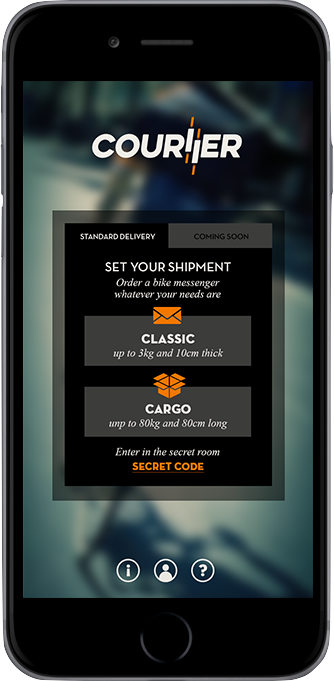
\includegraphics[width=.3\textwidth, frame]{Figures/ijil/courier1.png}
    }
    \hfill
    \subcaptionbox{Хүргэлтийн очих байршил сонгох}{
        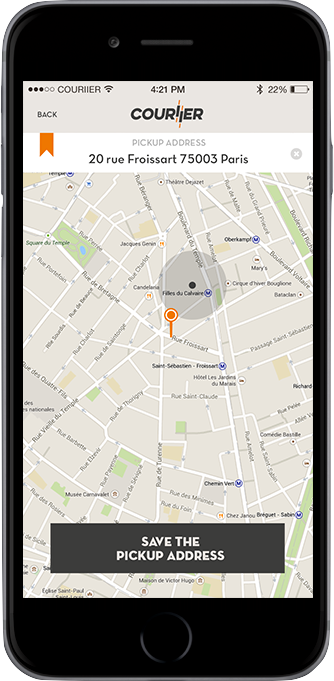
\includegraphics[width=.3\textwidth, frame]{Figures/ijil/courier2.png}
    }
    \hfill
    \subcaptionbox{Хүргэлтийн мэдээллүүд оруулах}{
        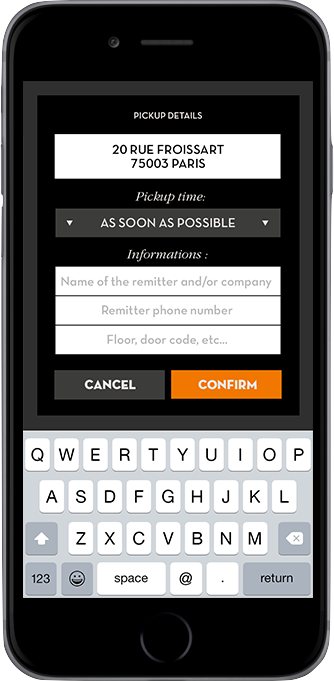
\includegraphics[width=.3\textwidth, frame]{Figures/ijil/courier3.png}
    }
	\caption{Courier аппликэйшны дэлгэцийн интерфэйс}
	\label{fig:courier}
\end{figure}


\subsection{DBike Messenger апп}
Уг аппын давуу талуудыг доор дурдвал.
\begin{enumerate}[noitemsep]
    \item Хүргэгч болон хэрэглэгч 2 хоорондоо чатлах боломжтой.
    \item Түүх харах боломжтой.
    \item Төлбөрийн системийг системд багтаасан.
    \item Мобайл апп-аас гадна вэб апптай.
\end{enumerate}

\noindent Сул талууд:
\begin{enumerate}[noitemsep]
    \item Үнийг хэрэглэгч биш систем тогтооно.
	\item Хэрэглэгчийн интерфэйс муутай.
	\item Хэтэрхий олон нэмэлттэй, хэрэглэхэд төвөгтэй.
	\item Зарим утасны хувилбар дээр ажиллах боломжгүй.
	\item Утас амархан ачаалладаг.
\end{enumerate}


Зураг~\ref{fig:dbike}--т DBike Messenger аппликэйшны дэлгэцүүдийг жишээ болгон харуулав.
\begin{figure}[H]
	\centering
    \subcaptionbox{Хүргэлтүүдийн жагсаалт}{
        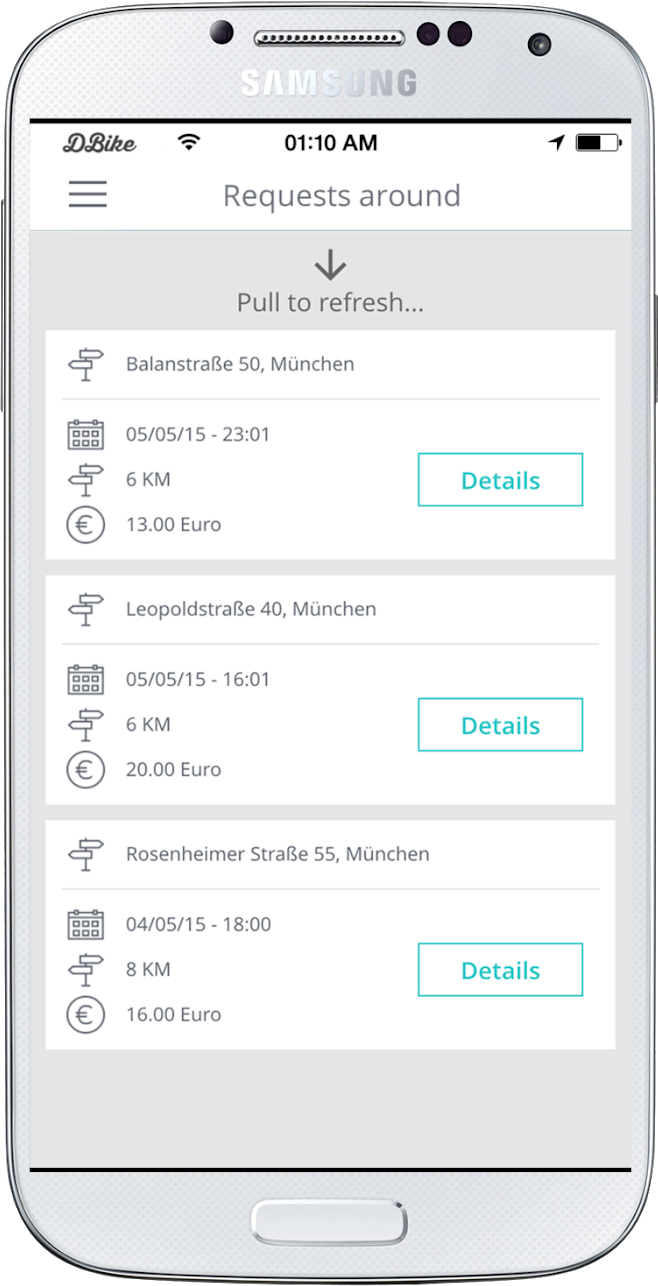
\includegraphics[width=.3\textwidth, frame]{Figures/ijil/dbike1.png}
    }
    \hfill
    \subcaptionbox{Хүргэлтийн дэлгэрэнгүй}{
        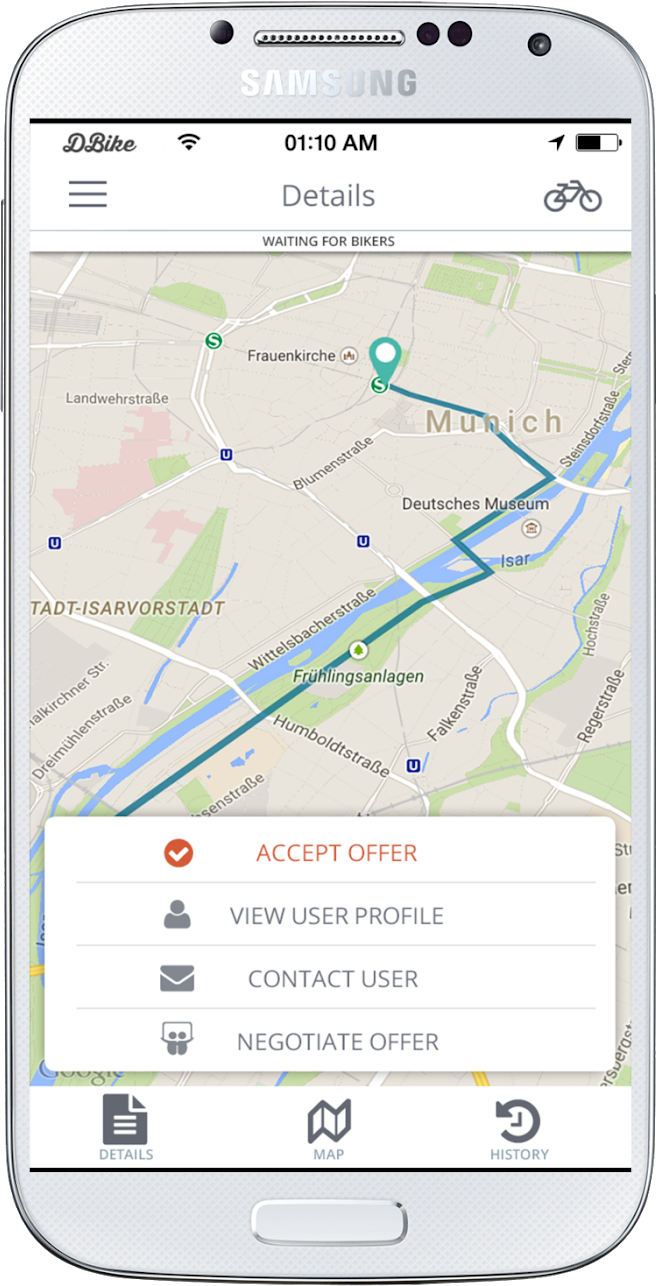
\includegraphics[width=.3\textwidth, frame]{Figures/ijil/dbike2.png}
    }
    \hfill
    \subcaptionbox{Хүргэлтийн төлөв өөрчлөх}{
        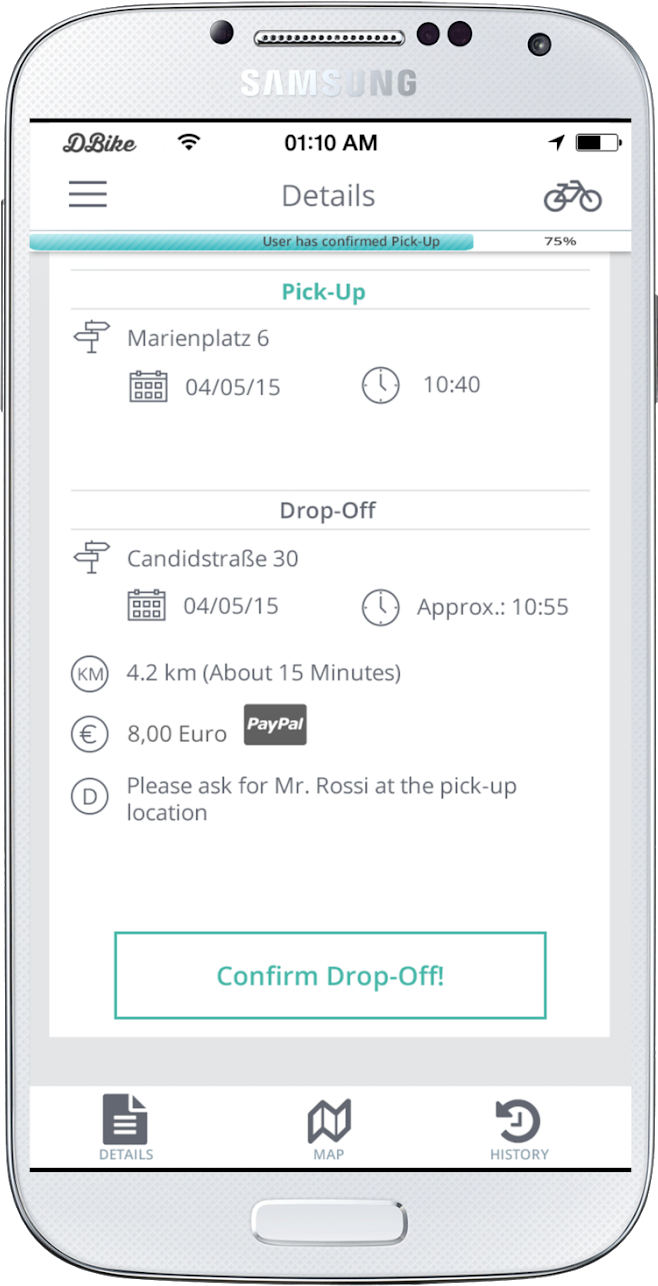
\includegraphics[width=.3\textwidth, frame]{Figures/ijil/dbike3.png}
    }
	\caption{DBike Messenger аппликэйшны дэлгэцийн интерфэйс}
	\label{fig:dbike}
\end{figure}



%---------------------------------------------------------------------------------------
%	SECTION 3
%---------------------------------------------------------------------------------------
\section{Тоон судалгаа баримт}

Зураг~\ref{fig:employee}--т АНУ-д үйл ажиллагаа явуулдаг хүргэлтийн байгууллагуудын ажилчдын тоон өсөлтийг харуулав.
\begin{figure}[H]
	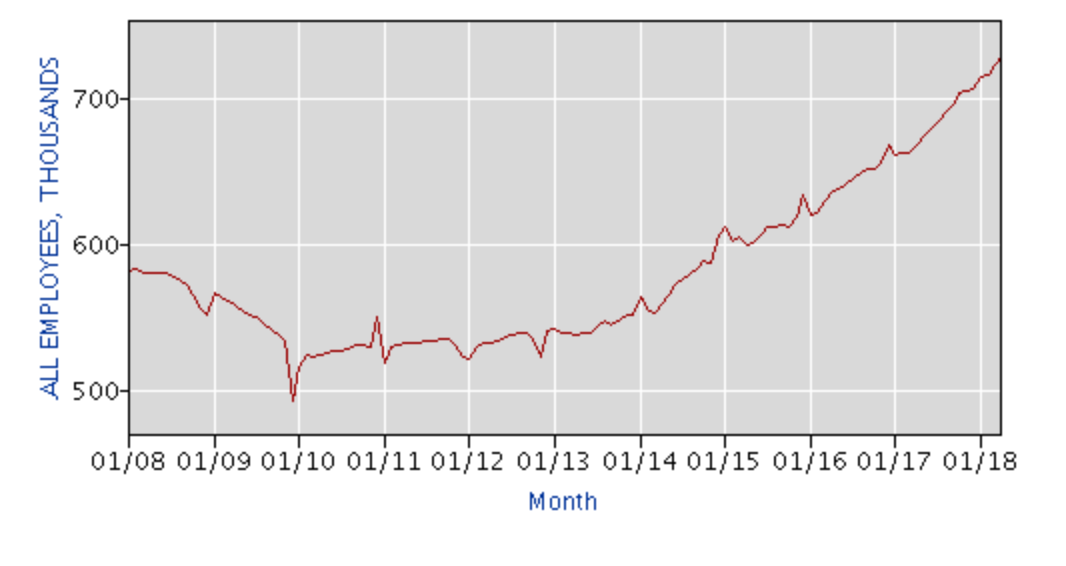
\includegraphics[width=\textwidth]{Figures/sudalgaa/employees.png}
	\caption{Хүргэлтийн үйлчилгээ үзүүлдэг байгууллагуудын ажилчдын тоон өсөлт}
	\label{fig:employee}
\end{figure}
Зураг~\ref{fig:earnings}--т АНУ-д үйл ажиллагаа явуулдаг хүргэлтийн байгууллагуудын ажилчдын цагийн цалингийн өөрчлөлтийг харуулав.
\begin{figure}[H]
	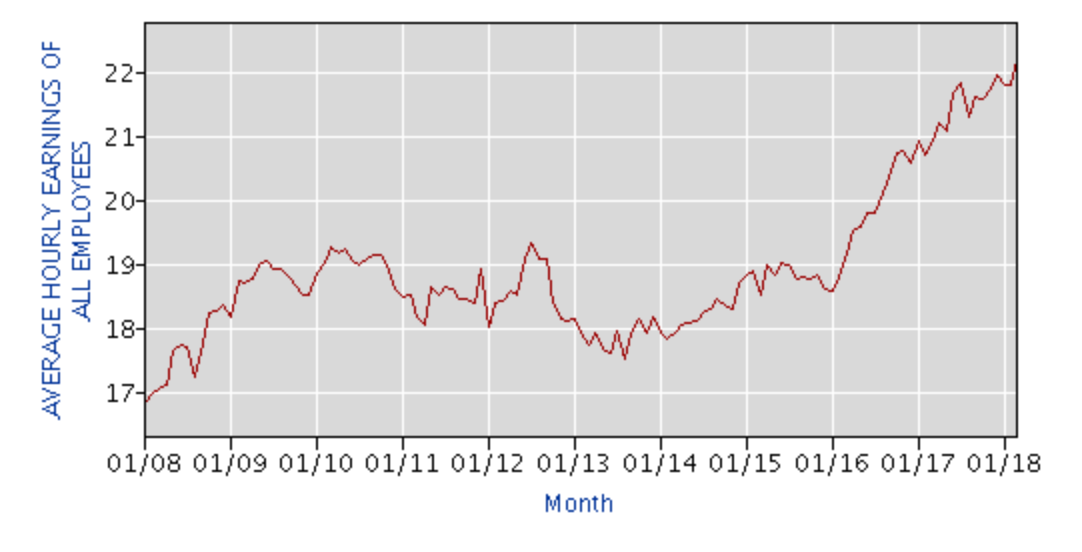
\includegraphics[width=\textwidth]{Figures/sudalgaa/earnings.png}
	\caption{Хүргэлтийн үйлчилгээ үзүүлдэг байгууллагуудын ажилчдын цагийн цалингийн өөрчлөлт\cite{Statics}}
	\label{fig:earnings}
\end{figure}

%---------------------------------------------------------------------------------------
%	SECTION 4
%---------------------------------------------------------------------------------------
\section{Хөгжүүлэлтэд ашиглах технологи, хэрэгслүүд}

\subsection{Риакт (React)-ын тухай}
Риакт (заримдаа React.js эсвэл ReactJS) нь хэрэглэгчийн интерфэйс бүтээхэд зориулсан ЖаваСкрифт сан юм.

Риактыг SPA болон мобайл аппликэйшн хийхэд ашиглаж болдог. Риактын гол баримтлал нь хурд, энгийн байдал болон өргөтгөх боломж юм. Риактыг өөр бусад сангуудтай өргөнөөр ашигладаг бөгөөд тэдгээрийн нэг нь Рэдүкс юм.

SPA (Single Page Application) нь энгийнээр вэб аппликешныг browser дотор ашиглах явцад хуудас дахин дууддагүй аппликешн юм. Таны өдөр бүр л хэрэглэдэг Gmail, Google Maps, Facebook г.м вэб аппликешнууд. SPA нь маш сайн UX -тэй ашиглахад таатай experience үзүүлэх, хуудас дахин дуудахгүй, контент хүлээх шаардлагагүй, доторх контентоо дээд түвшиний javascript фрэймворкууд (Angular, Ember, React)-ын тусламжтай дуудаж харуулдаг.

\subsubsection{Түүх}
Риактыг Фэйсбүүкийн програм хангамжийн инженер Жордан Валкэ нь анх бүтээсэн. Анх тэрээр PHP-д зориулсан HTML бүрэлдэхүүний фрэймворк гаргаж байсан. Үүнийг 2011 онд Фэйсбүүкийн мэдээний фийд дээр ашиглаж эхлэсэн бөгөөд хожим 2012 оноос Инстаграммд хэрэглэх болсон. Риактыг 2013 оны 5-р сард болсон JSConf арга хэмжээнд нээлттэй эх (opensource) болгосон.

\subsubsection{Ялгарах онцлог}
\begin{itemize}[label={--}]
    \item 1 чигийн өгөгдлийн холбоо (One-way data binding).
    \item Нөхцөлт бүрэлдэхүүнүүд.
    \item Хийсвэр DOM.
    \item Амьдралын цикл.
    \item JSX.
    \item HTML-ээс ангид архитектур.
\end{itemize}

\begin{figure}[H]
	\centering
	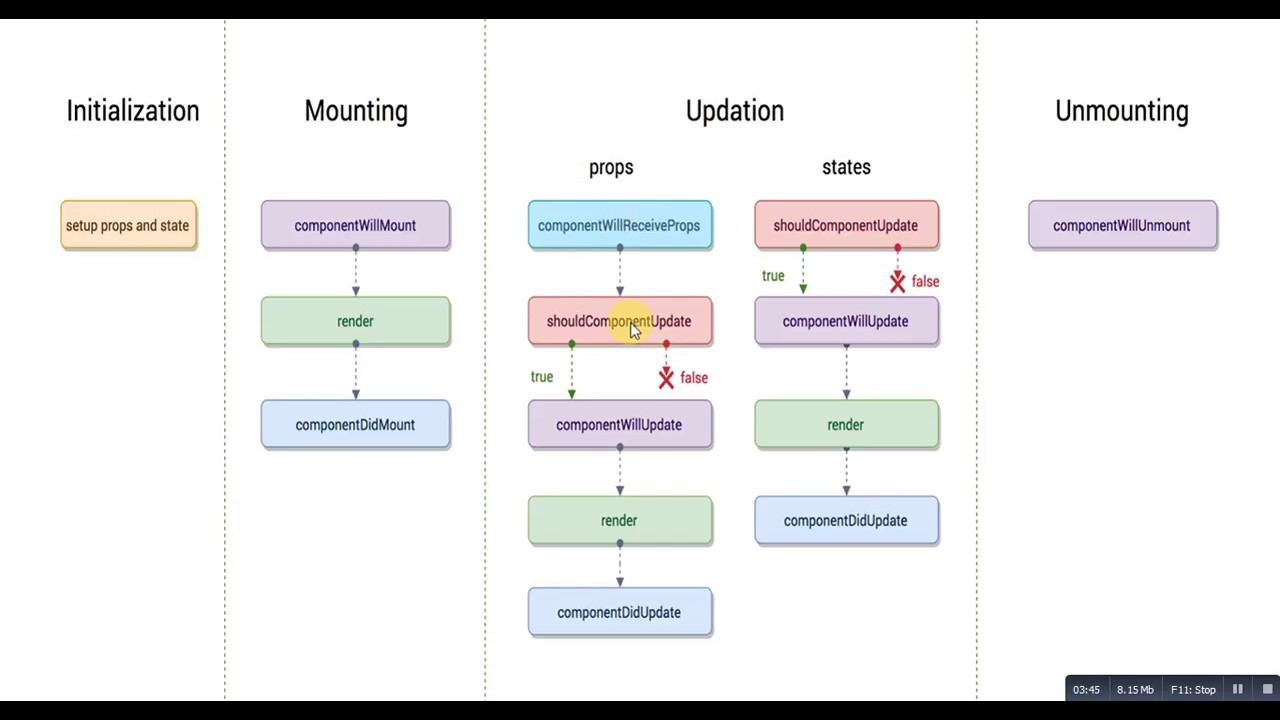
\includegraphics[width=\textwidth]{Figures/sudalgaa/react-lifecycle.jpg}
	\caption{Риакт амьдралын цикл}
	\label{figure:react-lifecycle}
\end{figure}

%----------------------------------------------------------------------
\subsection{Рэдүкс (Redux)-ын тухай}
Рэдүкс нь Жаваскрипт аппуудад зориулсан урдчилан таамаглах боломжтой нөхцөл агуулагч юм.

Рэдүкс нь апп-ны нөхцлүүдийг удирдахад илүү амар болгож өгнө. Өөрөөр хэлбэл хэрэглэгчийн үйлдэлд хэрхэн хариу өгч ямар өгөгдөл харуулахыг удирддаг.

\begin{figure}[H]
	\centering
	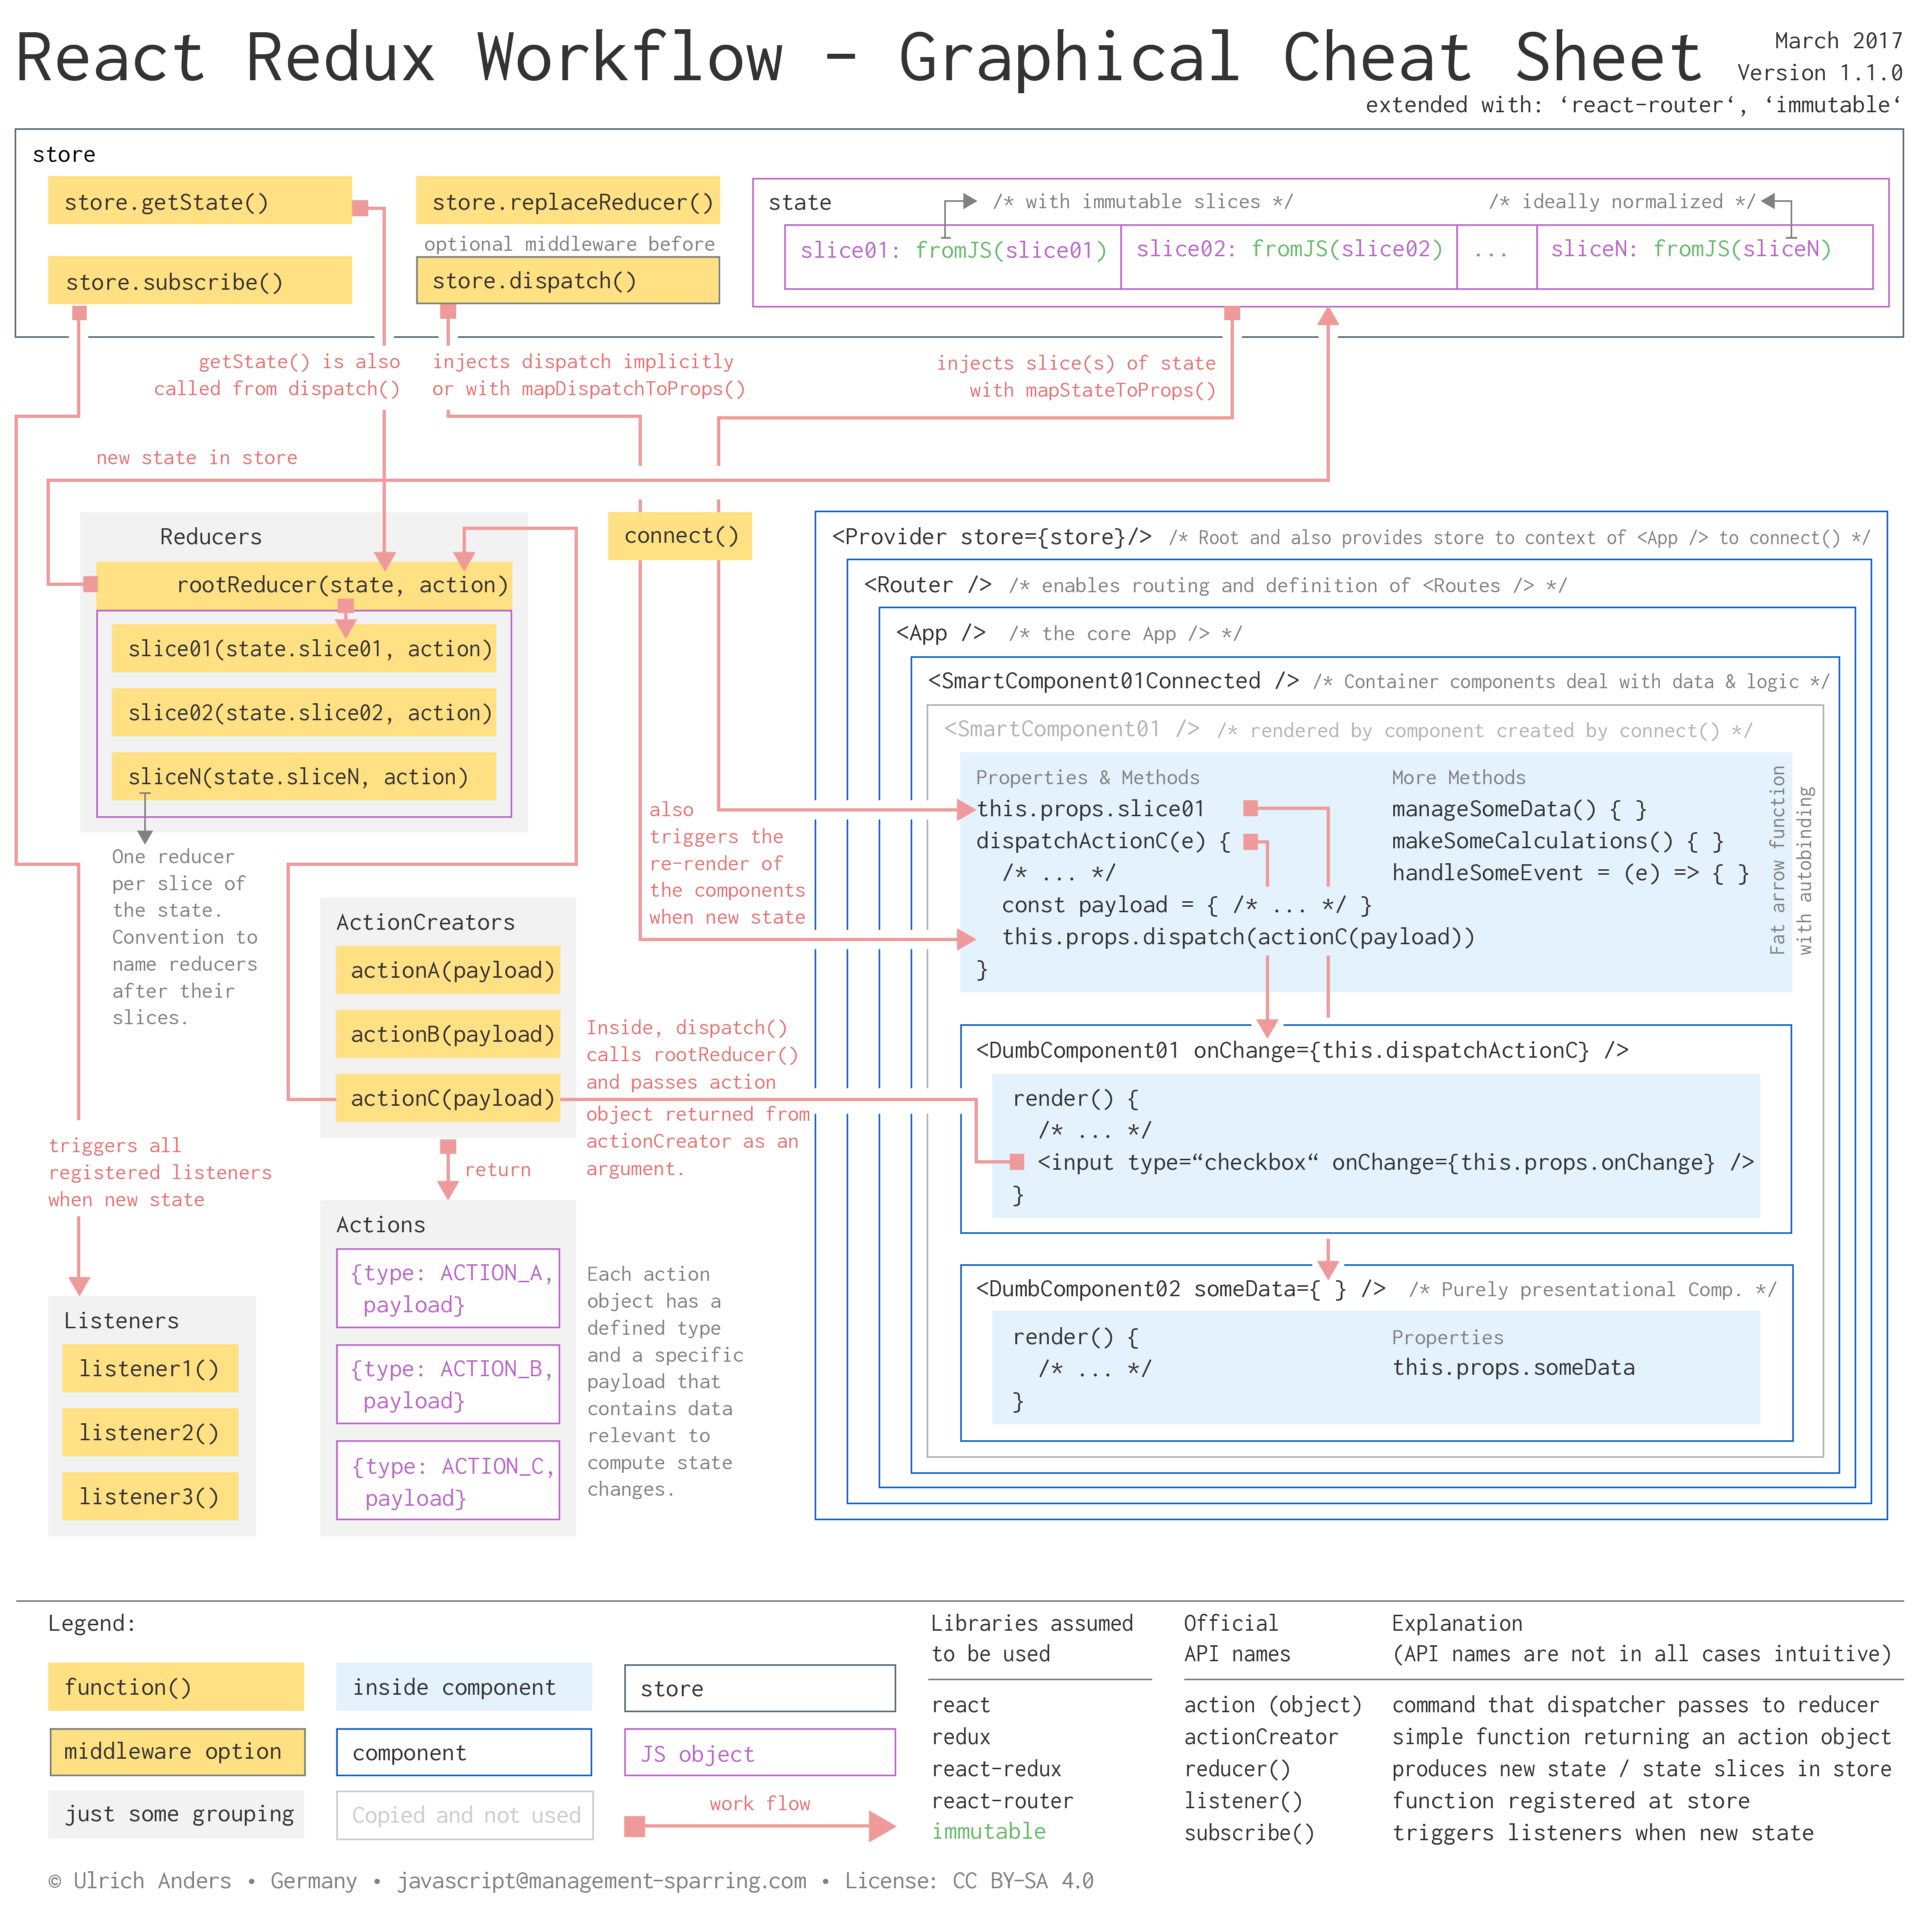
\includegraphics[width=\textwidth]{Figures/sudalgaa/redux-workflow.png}
	\caption{Рэдүкс ажиллах дараалал}
	\label{figure:redux-workflow}
\end{figure}

%----------------------------------------------------------------------
\subsection{Риакт Натив (React Native)-ын тухай}
Риакт Натив нь Жаваскрипт ашиглан мобайл апп хөгжүүлэх боломжийг олгодог. Риакттай яг адил загвар ашигладаг. Objective-C, Java, эсвэл Swift дээр бичсэн бүрэлдэхүүнүүдийг өөгүй нэгтгэнэ. Натийв код ашиглах хэрэг гарсан үед зарим талыг энгийнээр засаж болно. Апп-ны зарим хэсгийг Риакт натив ашиглан зарим хэсгийг Натийв код бичих боломжтой.

% ---------------------------------------------------------------------
\subsection{Экспо (Expo)-ын тухай}
Экспо апп нь Риакт Натийв апп бөгөөд дотроо Экспо SDK агуулна.Уг SDK нь native-and-JS сан бөгөөд төхөөрөмж (Камер, дугаарууд, өгөгдлийн хадгалалт, болон бусад техник хангамж) рүү хандах боломжийг олгодог. Энэ нь заавал натийв код бичихгүйгээр асуудлуудыг шийдэх боломжийг олгоно мөн төслийг зөвхөн Жаваскрипт ашиглан авсаархан байхад тусална. Экспо нь мөн хэрэглэгчийн түгээмэл боловч Риакт Натив үндсэн элементүүдэд байхгүй бүрэлдэхүүн хэсгүүдээр хангадаг. Жишээ нь: icon гэх мэт...

% ---------------------------------------------------------------------
\subsection{Фаирбейс платформ}
Гүүглэ компанийн Файрбейс (Firebase) нь гар утасны аппликейшн хөгжүүлэхэд шаардлагатай бүхий л үйлчилгээг нэг дор хослуулсан маш хүчирхэг платформ юм. 
\begin{figure}[H]
	\centering
	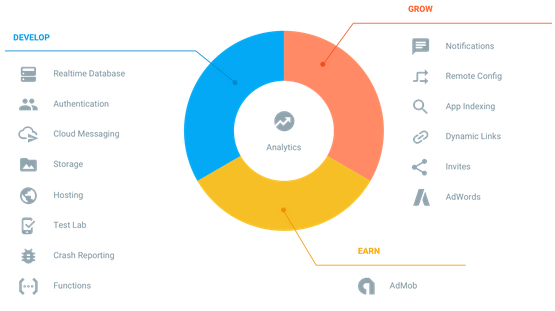
\includegraphics[width=\textwidth]{Figures/sudalgaa/firebase.png}
	\caption{Фаирбейс платформ}
	\label{figure:social}
\end{figure}

\subsubsection{Бодит хугацаатай өгөгдлийн сан}
Фаирбейс-ийн бодит хугацаатай өгөгдлийн сан (Real-time database) нь үүлэнд суурилдаг бөгөөд өгөгдлөө жей-сон форматаар хадгалаж синхроноор өгөгдлийн шинэчлэлтүүдийг системд холбогдсон бүхий л хэрэглэгчдэд хэдхэн миллисекундын дотор автоматаар хийдэг. 

\subsubsection{Хэрэглэгчийн найдвартай байдал}
Ихэнхи аппликейшны нэн тэргүүний хэрэгцээ бол хэрэглэгчдийн мэдээллийг аюулгүй , найдвартайгаар хадгалах юм. Фаирбейс-ийн хэрэглэгчийн найдвартай байдал буюу англиар Authentication нь энэхүү асуудлыг бүрэн цогцоор нь шийдвэрлэж өгсөн байдаг.

\subsubsection{Хадгалалт}
Хэрэглэгчидтэй холбоотой бүхий л төрлийн зураг, видео, файл зэргийг Фаирбейс-ийн хадгалалт(firebase storage) - ийн тусламжтайгаар үүлэнд хадгалах боломжтой байдаг. 

\begin{figure}[H]
	\centering
	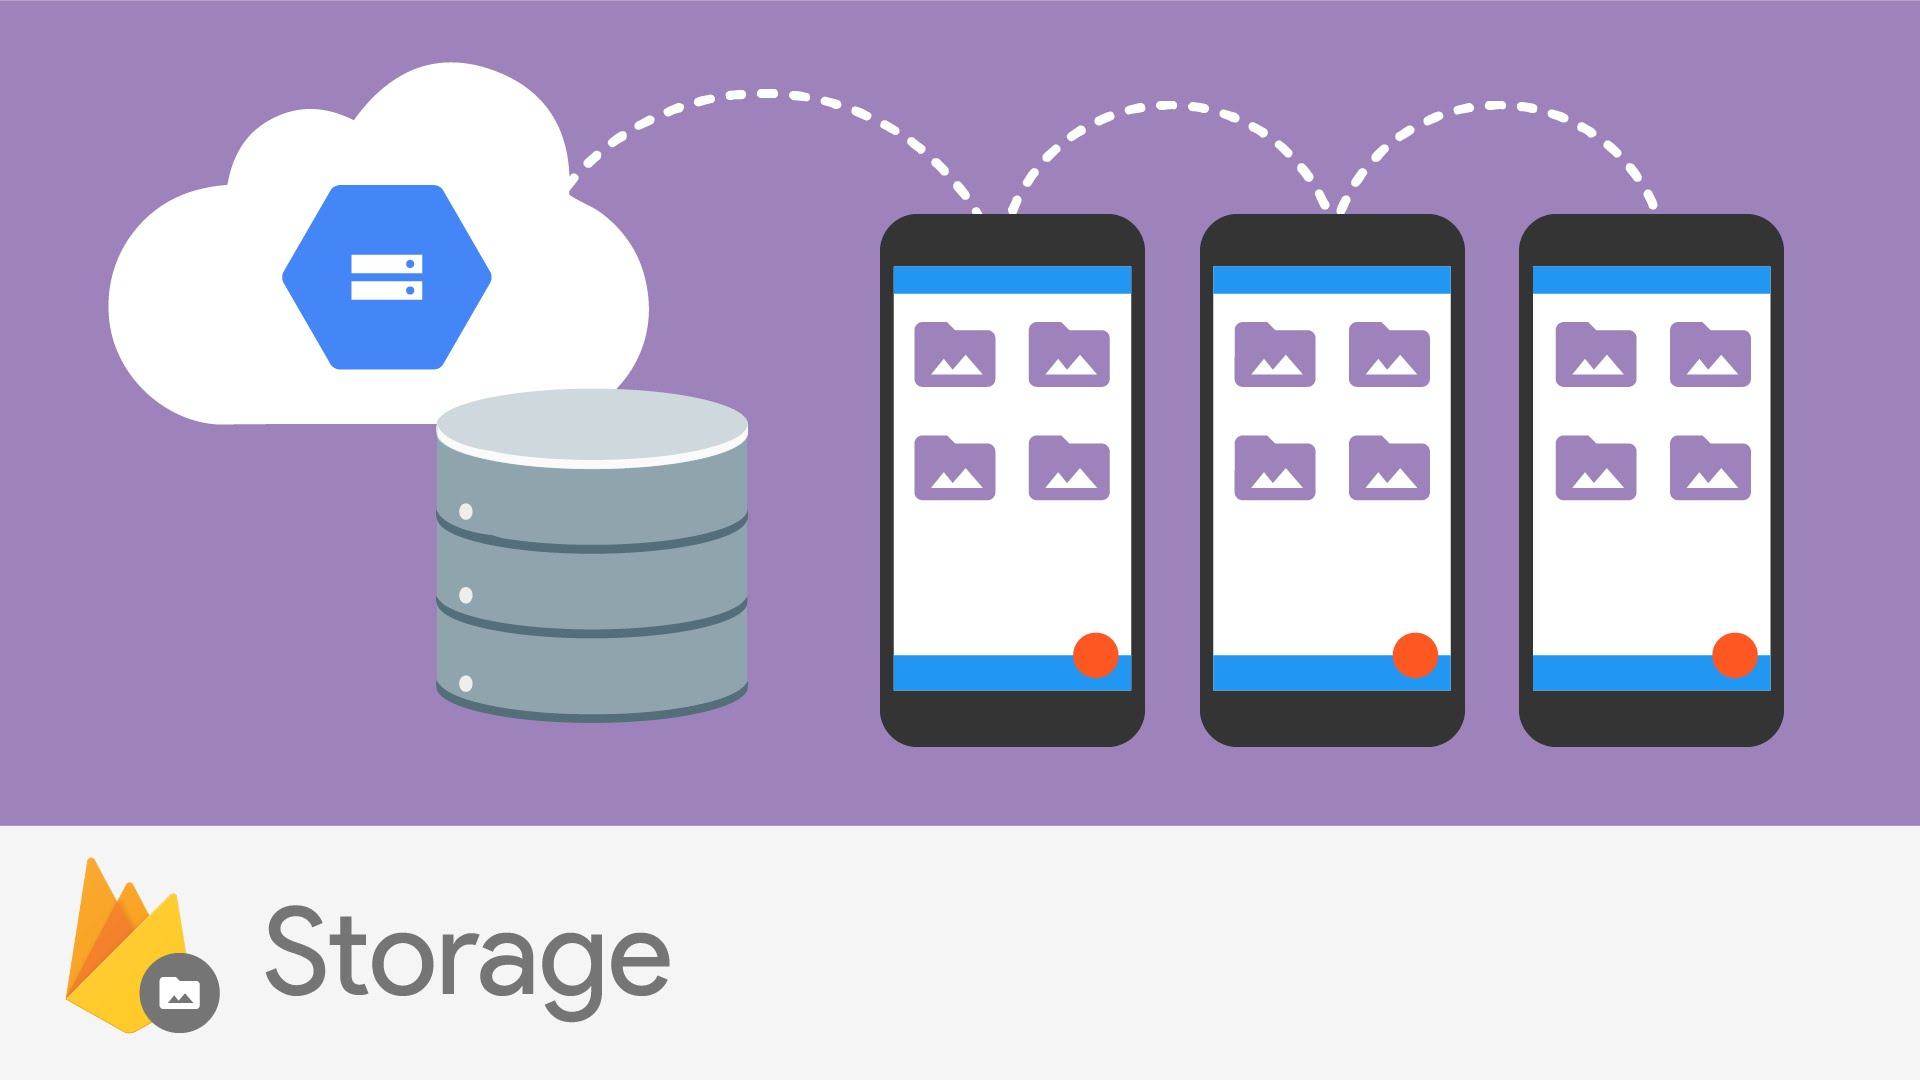
\includegraphics[width=\textwidth]{Figures/sudalgaa/firebaseStorage.jpg}
	\caption{Фаирбейс хадгалалт}
	\label{figure:storage}
\end{figure}

% ---------------------------------------------------------------------
\subsection{Гүүгл Мап (Google Maps)-ын тухай}
Уг Google Maps нь Гүүглэ компаний өөрсдийн газрын зургийг API түлхүүр үгээрээ дамжуулан серверээс өгөгдлөө аван аппликэйшндаа дүрслэх, дурын байршил заах, хэрэглэгчийн байршилын мэдээллийг координатаар тодорхойлох зэрэг үйлдлүүдийг гүйцэтгэж болохоос гадна бусад Google API-уудаар өргөтгөх боломжтой.
\begin{figure}[H]
    \centering
	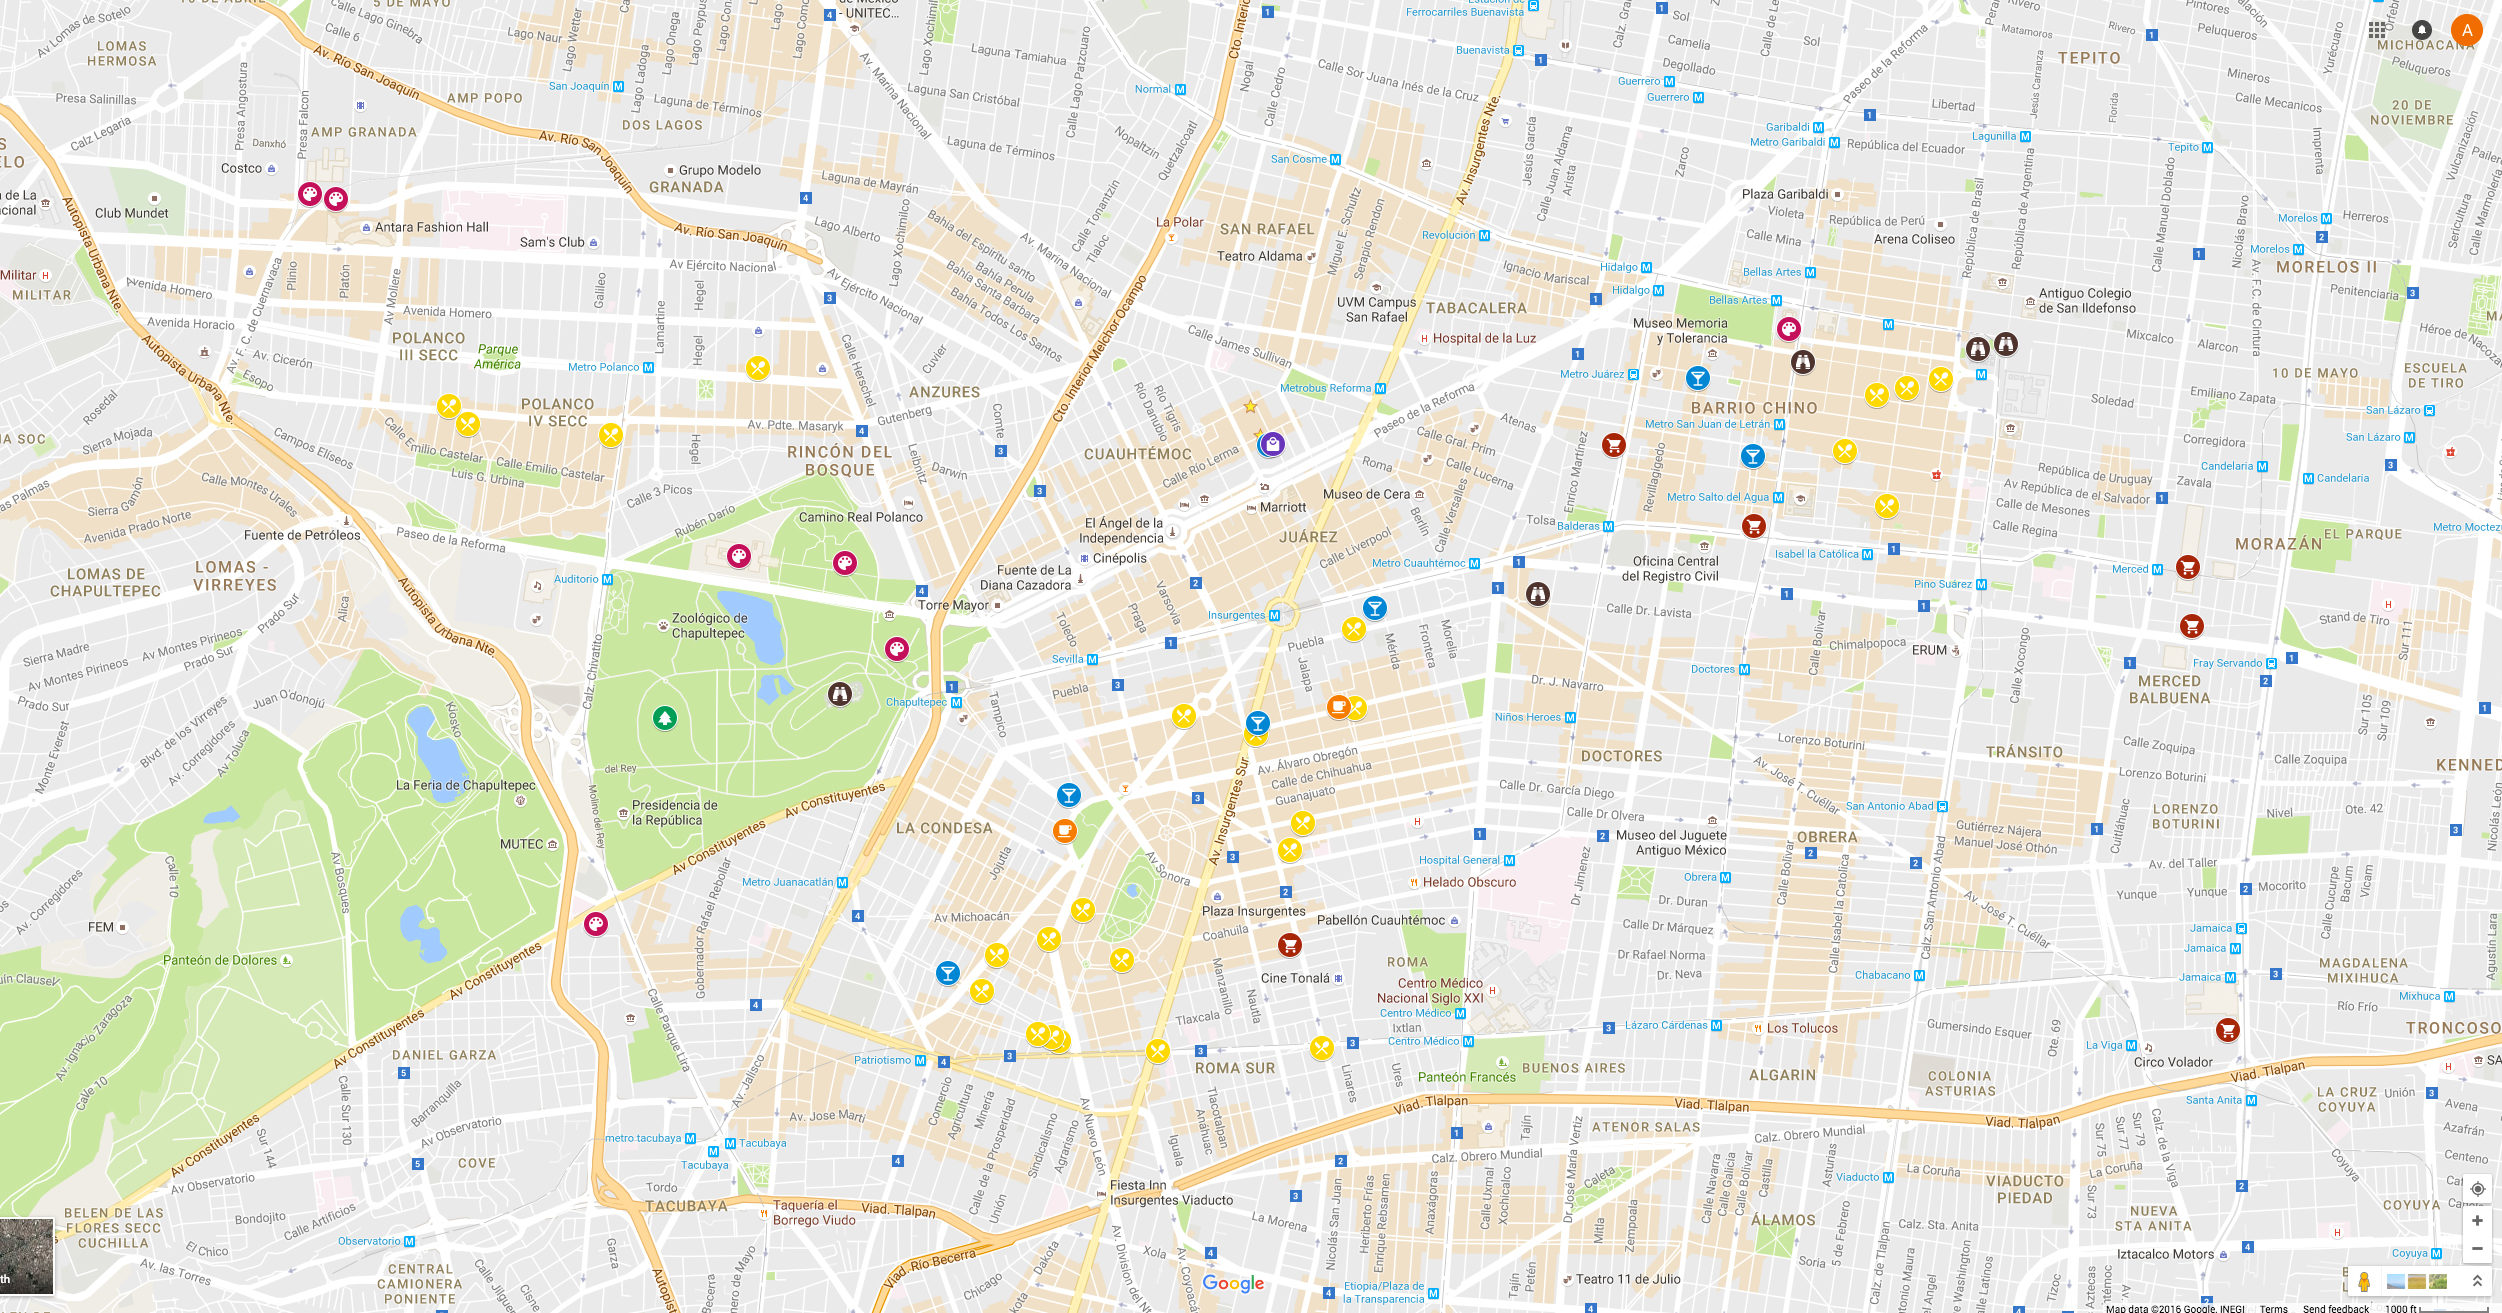
\includegraphics[width=\textwidth]{Figures/sudalgaa/Google-Maps.jpg}
	\caption{Google Maps харагдах байдал.}
	\label{fig:Google-Maps}
\end{figure}
Энэхүү програм хангамж хөгжүүлэх хэрэгслийг ашиглахын тулд Гүүглийн хөгжүүлэгчдийн сайтад нэвтэрч шинэ прожект үүсгэнэ. Дараа нь ашиглах API-аа сонгож API Key буюу түлхүүр үг үүсгэн хадгална.

%---------------------------------------------------------------------------------------
%	SECTION 5
%---------------------------------------------------------------------------------------
\section{Хөгжүүлэлтэнд ашиглах алгоритм}

\subsection{Хамгийн богино зам олох.}
Дээр дурдсан Google Direction API нь тодорхой хоёр байршил хоорондын хамгийн богино тодорхойлж өгдөг API юм.
Уг API-ийн ашиглаж байгаа хамгийн богино зам олох алгоритмууд нь олон тооны бөгөөд дэлхий нийтээр Дейкстра алгоритмыг ашигласан байх магадлал маш өндөр гэж үзэж байгаа.
Учир нь Дэйкстра алгоритм нь хамгийн сүүлийн үеийн хоёр байршил хоорондын хамгийн бага өртөгтэй замыг хайж олдог алгоритм юм.  

%---------------------------------------------------------------------------------------
%	SECTION 6
%---------------------------------------------------------------------------------------
\section{Бүлгийн дүгнэлт}

Энэ бүлгийн хүрээнд уг системийн судалгааны бичиг баримтыг хийж гүйцэтгэсэн ба дараах зүйлсийг тодорхойлов:
\begin{itemize}[label={--}]
    \renewcommand\labelitemi{--}
    \item Системийн тухай танилцуулгыг тодорхойлсон,
    \item Ижил төстэй системийн судалгааг хийсэн,
    \item Тоон судалгааг хийсэн,
    \item Хөгжүүлэлтэд ашиглагдах алгоритмыг тодорхойлсон,
    \item Хөгжүүлэлтэд ашиглах технологи, хэрэгслүүдийг тодорхойлсон болно.
\end{itemize}

%-------------------------------------------------------------------------------
    % Бүлэг 2

\pagecolor{ChapterYellow}
\chapter{Шаардлага ба шинжилгээ} % 2р бүлгийн гарчиг

\label{Chapter2} % Энэ бүлэг рүү ишлэл хийх бол \ref{Chapter2} командыг ашигла
%-------------------------------------------------------------------------------
%	SECTION 1
%-------------------------------------------------------------------------------
\pagecolor{white}
\section{Системийн үйл ажиллагаа}

Систем нь ямар нэг үйлчилгээний компанид зориулагдаагүй бөгөөд хүргэлтийн үйлчилгээ үзүүлдэг болон хувь хүн бүрд зориулагдсан ухаалаг систем юм. Системийг ашиглахын тулд хэрэглэгч интернет сүлжээнд холбогдсон байх ба системд бүртгэлтэй байх ёстой бөгөөд бүртгэлээ сошиал хаягаараа нээх аль эсвэл бүртгүүлэх форумыг бөглөж бүртгүүлнэ. Систем нь хүргэгч болон үйлчлүүлэгч гэсэн үндсэн хоёр хэрэглэгчтэй. Үйлчлүүлэгч нь хүргүүлэх үйлчилгээг өөрийн байгаа байршил дээр захиалж болно.\\
\textit{\textbf{Хүргэлтийн үйлчилгээ захиалах:}}\\
Хэрэглэгч хүргэлтийн мэдээллүүдээ системд оруулна ингэснээр захиалгыг бүртгэх ба хүргэгч нийт захиалга дундаас өөрийн хүссэн захиалгыг сонгон хүргэх боломжтой.\\
\textit{\textbf{Хүргэлтийн үйлчилгээ цуцлах:}}\\
Хэрэв хүргэлтийг хүргэж эхлээгүй бол хэрэглэгч үйлчилгээгээ цуцлаж хүргүүлэх хүсэлтээ устгах боломжтой.\\
\textit{\textbf{Хүргэлтийн үйлчилгээг дуусгах:}}\\
Хүргэгч хэрэв хүргэлтийг хүргэж өгсөн бол хүргэлтийг дуусгасан гэж тэмдэглэнэ.\\
\textit{\textbf{Хүргэгчийг үнэлэж оноо өгөх:}}\\
Хүргэгч хүргэлтийг хүргэж өгсөн бол үйлчлүүлэгч хүргэгчид үнэлгээ өгөх эрхтэй болно.\\
\textit{\textbf{Хэрэглэгчийн мэдээлэл шинэчлэх:}}\\
Хэрэглэгч систем өөрийн утас болон зураг нэрийг оруулах бөгөөд эдгээр мэдээллүүдийг дараа нь шинэчлэх боломжтой байна.

%-----------------------------------
%	SECTION 2
%-----------------------------------

\section{Системийг ашиглах хэрэглэгчид}

\subsection{Системийн оролцогч}
\begin{enumerate} 
    \item \textit{Хэрэглэгчид} - Системээр дамжуулан хүргэлтийн үйлчилгээг авах, эсвэл хүргэлтийн үйлчилгээ үзүүлэх хүсэлтэй хувь хүмүүс.
\end{enumerate}

\subsection{Системийн тоглогч}
\begin{enumerate}
    \item \textit{Үйлчлүүлэгч} - Системээр дамжуулан хүргэлтийн үйлчилгээг авах хүсэлтэй иргэн.
    \item \textit{Хүргэгч} - Системээр дамжуулан хүргэлтийн үйлчилгээ үзүүлэх хүсэлтэй иргэн.
\end{enumerate}

%-----------------------------------
%	SECTION 3
%-----------------------------------

\section{Функцийн шаардлага}

\begin{enumerate}
    \item Систем нь үйлчлүүлэгч болон жолооч гэсэн үндсэн 2 модультай байна.
    \item Хэрэглэгч хувийн мэдээллээ оруулан системд бүртгүүлнэ.
    \item Хэрэглэгч нь сошиал хаягаараа нэвтрэх орох боломжтой байна.
    \item Систем нь үйлчилгээ дууссаны дараа жолооч болон үйлчлүүлэгчдийн харилцаа үйлчилгээний үнэлгээг 1-ээс 5 одоор болон текст хэлбэрээр үнэлгээг авдаг байна.
    \item Системд хэрэглэгчээр бүртгүүлэхдээ нэр, зураг болон утасны дугаараа бүртгүүлнэ.
    \item Систем нь хүргэгчид хүргэлтийн цэг рүү очих хамгийн богино замыг зааж харуулдаг байна.
    \item Хүргэгч нь үйлчлүүлэгчийн захиалгыг гүйцэтгэсний дараа үйлчлүүлэгч үнэлгээ өгдөг байна.
\end{enumerate}
%-----------------------------------
%	SECTION 4
%-----------------------------------

\section{Функцийн бус шаардлага}
\begin{itemize}
	\item Гүйцэтгэлийн шаардлага:
	\begin{enumerate}
		\item Хурдан ажилладаг байх;
		\item Найдвартай ажиллагаатай байх;
	\end{enumerate}
	\item Интерфэйсийн шаардлага:
	\begin{enumerate}
	    \item Хэрэглэхэд ойлгомжтой энгийн байх;
	\end{enumerate}
	\item Аюулгүй байдлын шаардлага: 
	\begin{enumerate}
	    \item Найдвартай ажиллагаатай байх;
 		\item Хэрэглэгчийн мэдээллийг алдахгүй байх ;
	\end{enumerate}
 	\item Нууцлалын шаардлага:
 	\begin{enumerate}
 		\item Хэрэглэгч нэвтрэх бүртгүүлэх боломжтой байх;
 	\end{enumerate}
\end{itemize}

%-----------------------------------
%	SECTION 5
%-----------------------------------
\section{Юзкейс диаграм}
\begin{figure}[H]
	\centering
	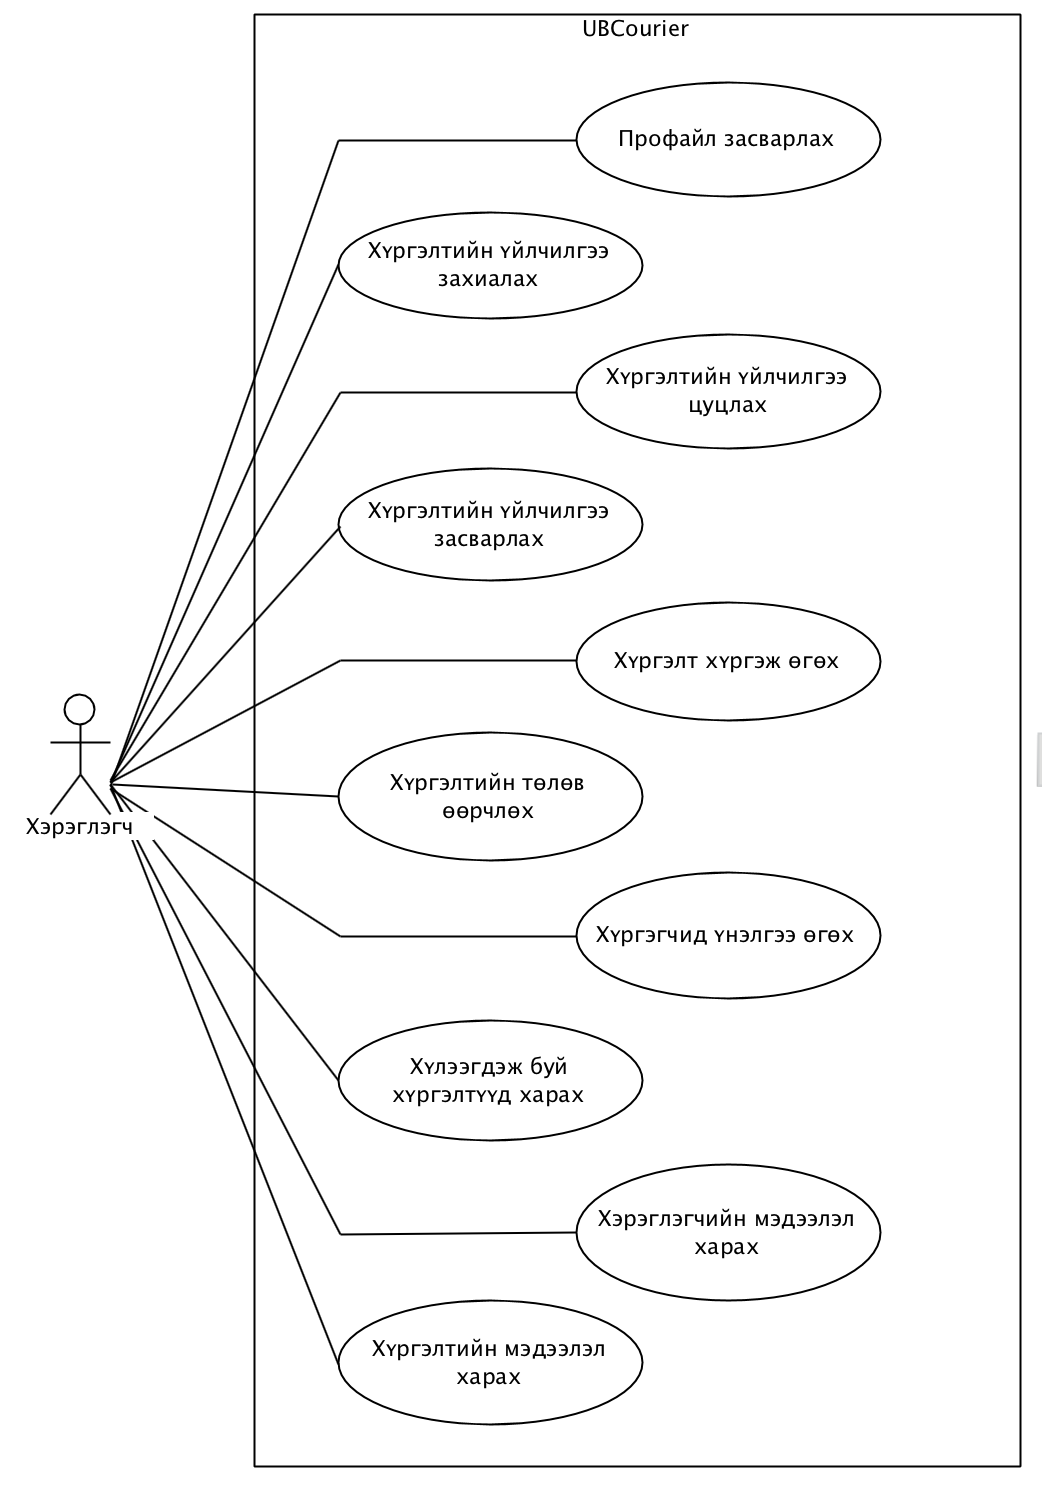
\includegraphics[width=\textwidth]{Figures/shinjilgee/usecase.png}
	\caption{Юзкейс диаграм}
\end{figure}

%-----------------------------------
%	SECTION 6
%-----------------------------------

\section{Юзкейс тодорхойлолт}

\begin{table}[H]
    \caption{Профайл засварлах юзкейс тодорхойлолт}
    \begin{tabular}{|l|p{9cm}|}
		\hline
		{\bfseries Юзкейс:} & Профайл засварлах \\\hline
		{\bfseries ID:} & 1 \\\hline
		{\bfseries Эрэмбэ:} & Өндөр \\\hline
		{\bfseries Үндсэн тоглогч:} & Хэрэглэгч \\\hline
		{\bfseries Нэмэлт тоглогч:} & Байхгүй. \\\hline
		{\bfseries Товч тайлбар:} & Хэрэглэгч өөрийн мэдээллүүдийг засварлах. \\\hline
		{\bfseries Триггер:} & Хэрэглэгч профайл засварлах. \\\hline
		{\bfseries Өмнөх нөхцөл:} & 
		    \begin{enumerate}[nosep]
		        \item Хэрэглэгч өөрийн эрхээр нэвтэрсэн байх.
		        \item Өөрийн профайл руу орсон байх.
		    \end{enumerate}
		\\\hline
		{\bfseries Үндсэн урсгал:} &
			1.0
			\begin{enumerate}[nosep]
				\item IF (Профайл засварлах товчийг дарна)
				    \begin{enumerate}[nosep]
				        \item Бүх мэдээлэл жагсаалт хэлбэрээр гарна.
                        \item Хэрэглэгч мэдээллүүдээ засварлана.
				    \end{enumerate}
				\item IF (Хадгалах товчийг сонговол)
				    \begin{enumerate}[nosep]
				        \item Хэрэглэгчийн мэдээллүүдийг хадгална.
				        \item Хэрэглэгчийн профайл руу буцна.
				    \end{enumerate}
			\end{enumerate}
		\\\hline
		{\bfseries Дараах нөхцөл:} &
		    \begin{enumerate}[nosep]
		        \item Өгөгдлийн санд мэдээллүүдийг хадгална.
		    \end{enumerate}
		\\\hline
		{\bfseries Альтернатив урсгал:} & Байхгүй \\
		\hline
    \end{tabular}
\end{table}

\begin{table}[H]
    \caption{Хүргэлтийн үйлчилгээ захиалах юзкейс тодорхойлолт}
    \begin{tabular}{|l|p{9cm}|}
		\hline
		{\bfseries Юзкейс:} & Хүргэлтийн үйлчилгээ захиалах \\\hline
		{\bfseries ID:} & 2 \\\hline
		{\bfseries Эрэмбэ:} & Өндөр \\\hline
		{\bfseries Үндсэн тоглогч:} & Хэрэглэгч \\\hline
		{\bfseries Нэмэлт тоглогч:} & Байхгүй \\\hline
		{\bfseries Товч тайлбар:} & Шинэ хүргэлт үүсгэх. \\\hline
		{\bfseries Триггер:} & Хэрэглэгч эд зүйл хүргүүлэх хэрэгцээ гарсан. \\\hline
		{\bfseries Өмнөх нөхцөл:} &
		    \begin{enumerate}[nosep]
		        \item Хэрэглэгч өөрийн эрхээр нэвтэрсэн байх.
		        \item Өөрийн хүргэлт цэс рүү орсон байх.
		    \end{enumerate}
		\\\hline
		{\bfseries Үндсэн урсгал:} &
			2.0
			\begin{enumerate}[nosep]
				\item IF (Шинээр хүргэлт үүсгэх товч дээр дарвал)
				    \begin{enumerate}[nosep]
				        \item Хүргэлтийн мэдээллүүд оруулах форм харагдана.
				        \item Хэрэглэгч мэдээллүүдийг бөгөлнө.
				    \end{enumerate}
				\item IF (Хадгалах товч дээр дарвал)
				    \begin{enumerate}[nosep]
				        \item Хүргэлтийн мэдээллүүдийг хадгална.
				        \item Хэрэглэгчийн хүргэлтүүдийн жагсаалт руу буцна.
				    \end{enumerate}
			\end{enumerate}
		\\\hline
		{\bfseries Дараах нөхцөл:} &
		    \begin{enumerate}[nosep]
		        \item Өгөгдлийн санд хүргэлтийг хадгална.
		        \item Шинэ хүргэлт нэмэгдэнэ.
		    \end{enumerate}
		\\\hline
		{\bfseries Альтернатив урсгал:} & Байхгүй
		\\\hline
    \end{tabular}
\end{table}

\begin{table}[H]
    \caption{Хүргэлтийн үйлчилгээ цуцлах юзкейс тодорхойлолт}
    \begin{tabular}{|l|p{9cm}|}
		\hline
		{\bfseries Юзкейс:} & Хүргэлтийн үйлчилгээ цуцлах \\\hline
		{\bfseries ID:} & 3 \\\hline
		{\bfseries Эрэмбэ:} & Өндөр \\\hline
		{\bfseries Үндсэн тоглогч:} & Хэрэглэгч \\\hline
		{\bfseries Нэмэлт тоглогч:} & Байхгүй \\\hline
		{\bfseries Товч тайлбар:} & Хүргэлт устгах.\\\hline
		{\bfseries Триггер:} & Хэрэглэгч хүргэлт устгах хэрэгцээ гарсан. \\\hline
		{\bfseries Өмнөх нөхцөл:} &
		    \begin{enumerate}[nosep]
		        \item Хэрэглэгч өөрийн эрхээр нэвтэрсэн байх.
		        \item Устгахын тулд хүргэлт үүсгэсэн байх.
		    \end{enumerate}
		\\\hline
		{\bfseries Үндсэн урсгал:} &
			3.0
			\begin{enumerate}[nosep]
				\item IF (Өөрийн үүсгэсэн хүртгэлт засварлах дээр дарвал)
				    \begin{enumerate}[nosep]
				        \item Хүргэлтийн мэдээллүүд харагдана.
				        \item IF (Хэрэглэгч хүргэлт устгах товч дээр дарвал.)
                        \begin{enumerate}[nosep]
                            \item Хэрэглэгчийн хүргэлтүүдийн жагсаалтруу буцна.
                            \item Хэрэглэгчийн усгахыг хүссэн хүргэлт устана.
                        \end{enumerate}
				    \end{enumerate}
			\end{enumerate}
		\\\hline
		{\bfseries Дараах нөхцөл:} &
		    \begin{enumerate}[nosep]
		        \item Өгөгдлийн сангаас хүргэлтийг устгана.
		        \item Хэрэглэгчийн усгахыг хүссэн хүргэлт устана.
		    \end{enumerate}
		\\\hline
		{\bfseries Альтернатив урсгал:} & Байхгүй
		\\\hline
    \end{tabular}
\end{table}

\begin{table}[H]
    \caption{Хүргэлтийн үйлчилгээ засварлах юзкейс тодорхойлолт}
    \begin{tabular}{|l|p{9cm}|}
		\hline
		{\bfseries Юзкейс:} & Хүргэлтийн үйлчилгээ засварлах \\\hline
		{\bfseries ID:} & 4 \\\hline
		{\bfseries Эрэмбэ:} & Дунд \\\hline
		{\bfseries Үндсэн тоглогч:} & Хэрэглэгч \\\hline
		{\bfseries Нэмэлт тоглогч:} & Байхгүй \\\hline
		{\bfseries Товч тайлбар:} & Хэрэглэгч өөрийн хүргэлтийн мэдээллээ засварлах.\\\hline
		{\bfseries Триггер:} & Хэрэглэгч өөрийн хүргэлтийн мэдээллээ засварлах хэрэгцээ гарсан. \\\hline
		{\bfseries Өмнөх нөхцөл:} &
		    \begin{enumerate}[nosep]
		        \item Хэрэглэгч өөрийн бүртгэлээр нэвтэрч орсон байх.
		        \item Хэрэглэгчийн засварлах хүргэлтийг хүргэгч хүргэж эхлээгүй байх.
		    \end{enumerate}
		\\\hline
		{\bfseries Үндсэн урсгал:} &
			4.0
			\begin{enumerate}[nosep]
			    \item Хэрэглэгч өөрийн хүргэлтийг засварлах товч дээр дарна.
			    \item Хүргэлтийн мэдээллүүд жагсаалт байдлаар харагдана.
			    \item Хэрэглэгч засварлахыг хүссэн мэдээллүүдээ засна.
				\item IF (Хадгалах дарвал)
				    \begin{enumerate}[nosep]
				        \item Хүргэлтийн мэдээллүүдийг хадгална.
				    \end{enumerate}
			\end{enumerate}
		\\\hline
		{\bfseries Дараах нөхцөл:} &
		    \begin{enumerate}[nosep]
		        \item Хэрэглэгчийн засварласан хүргэлтийн мэдээллийг хадгална.
		        \item Хэрэглэгчийн хүргэлтийн жагсаалтуудыг харуулна.
		    \end{enumerate}
		\\\hline
		{\bfseries Альтернатив урсгал:} & Байхгүй
		\\\hline
    \end{tabular}
\end{table}


\begin{table}[H]
    \caption{Хүргэлт хүргэж өгөх юзкейс тодорхойлолт}
    \begin{tabular}{|l|p{9cm}|}
		\hline
		{\bfseries Юзкейс:} & Хүргэлт хүргэж өгөх \\\hline
		{\bfseries ID:} & 5 \\\hline
		{\bfseries Эрэмбэ:} & Өндөр \\\hline
		{\bfseries Үндсэн тоглогч:} & Хэрэглэгч \\\hline
		{\bfseries Нэмэлт тоглогч:} & Байхгүй \\\hline
		{\bfseries Товч тайлбар:} & Хүргэгч хүргэлтийг авах.\\\hline
		{\bfseries Триггер:} & Хүргэгч хүргэлтийг хүргэж өгөх хүсэлтэй байх. \\\hline
		{\bfseries Өмнөх нөхцөл:} &
		    \begin{enumerate}[nosep]
		        \item Хэрэглэгч өөрийн эрхээр нэвтэрсэн байх.
		        \item Хүргэж өгөх хүргэлт рүү орсон байх.
		    \end{enumerate}
		\\\hline
		{\bfseries Үндсэн урсгал:} &
			6.0
			\begin{enumerate}[nosep]
			    \item Хүргэгчид хүргэлтийн мэдээллүүдийг харуулна.
			    \item Хүргэгч "хүргэж өгөх" товч дээр дарна.
			    \item Хүргэгчийн хүргэлтүүд рүү буцна.
			\end{enumerate}
		\\\hline
		{\bfseries Дараах нөхцөл:} &
		    \begin{enumerate}[nosep]
		        \item Өгөгдлийн санд хүргэлтийг хүргэгч дээр бүртгэнэ.
		    \end{enumerate}
		\\\hline
		{\bfseries Альтернатив урсгал:} & Байхгүй
		\\\hline
    \end{tabular}
\end{table}

\begin{table}[H]
    \caption{Хүргэгчид үнэлгээ өгөх юзкейс тодорхойлолт}
    \begin{tabular}{|l|p{9cm}|}
		\hline
		{\bfseries Юзкейс:} & Хүргэгчид үнэлгээ өгөх \\\hline
		{\bfseries ID:} & 7 \\\hline
		{\bfseries Эрэмбэ:} & Өндөр \\\hline
		{\bfseries Үндсэн тоглогч:} & Хэрэглэгч \\\hline
		{\bfseries Нэмэлт тоглогч:} & Байхгүй \\\hline
		{\bfseries Товч тайлбар:} & Хүргэлтийн үйлчилгээ захиалсан хэрэглэгч хүргэгчид үнэлгээ өгөх.\\\hline
		{\bfseries Триггер:} & Хүргэгч хүргэлтийг очих ёстой газар нь хүргэсэн байх. \\\hline
		{\bfseries Өмнөх нөхцөл:} &
		    \begin{enumerate}[nosep]
		        \item Хэрэглэгч өөрийн эрхээр нэвтэрсэн байх.
		        \item Хүргэж өгсөн хүргэлт рүү орсон байх.
		    \end{enumerate}
		\\\hline
		{\bfseries Үндсэн урсгал:} &
			7.0
			\begin{enumerate}[nosep]
			    \item Хүргэлтийн мэдээллүүдийг харуулна.
			    \item Хэрэглэгч хүргэгчид үнэлгээ өгөх товчийг дарна.
			    \item Хэрэглэгчид үнэлгээ өгөх цонхийг харуулна.
			    \item Хэрэглэгч хүргэгчид үнэлгээг 1-5 одоор мөн текстээр өгнө.
			\end{enumerate}
		\\\hline
		{\bfseries Дараах нөхцөл:} &
		    \begin{enumerate}[nosep]
		        \item Өгөгдлийн санд үнэлгээг хадгална.
		        \item Хүргэлтүүдийн жагсаалт руу буцна.
		    \end{enumerate}
		\\\hline
		{\bfseries Альтернатив урсгал:} & Байхгүй
		\\\hline
    \end{tabular}
\end{table}

\begin{table}[H]
    \caption{Хүлээгдэж буй хүргэлтүүд харах юзкейс тодорхойлолт}
    \begin{tabular}{|l|p{9cm}|}
		\hline
		{\bfseries Юзкейс:} & Хүлээгдэж буй хүргэлтүүд харах \\\hline
		{\bfseries ID:} & 8 \\\hline
		{\bfseries Эрэмбэ:} & Өндөр \\\hline
		{\bfseries Үндсэн тоглогч:} & Хэрэглэгч \\\hline
		{\bfseries Нэмэлт тоглогч:} & Байхгүй \\\hline
		{\bfseries Товч тайлбар:} & Хүргэгч хүргэж эхлээгүй хүлээгдэж буй хүргэлтүүд харах. \\\hline
		{\bfseries Триггер:} & Хүргэгч хүлээгдэж буй хүргэлтүүдийг харах хүсэлтэй байх. \\\hline
		{\bfseries Өмнөх нөхцөл:} &
		    \begin{enumerate}[nosep]
		        \item Хэрэглэгч өөрийн эрхээр нэвтэрсэн байх.
		        \item Цэснээс нүүр цэсийг сонгох.
		    \end{enumerate}
		\\\hline
		{\bfseries Үндсэн урсгал:} &
			8.0
			\begin{enumerate}[nosep]
				\item IF (Хүлээгдэж буй хүргэлтүүд байвал)
				    \begin{enumerate}[nosep]
		                \item Хүлээгдэх буй хүргэлтүүдийг харуулна.
				    \end{enumerate}
				\item ELSE
				    \begin{enumerate}[nosep]
		                \item Юу ч харуулахгүй.
				    \end{enumerate}
			\end{enumerate}
		\\\hline
		{\bfseries Дараах нөхцөл:} & Байхгүй \\\hline
		{\bfseries Альтернатив урсгал:} & Байхгүй \\\hline
    \end{tabular}
\end{table}

\begin{table}[H]
    \caption{Хэрэглэгчийн мэдээлэл харах юзкейс тодорхойлолт}
    \begin{tabular}{|l|p{9cm}|}
		\hline
		{\bfseries Юзкейс:} & Хэрэглэгчийн мэдээлэл харах \\\hline
		{\bfseries ID:} & 9 \\\hline
		{\bfseries Эрэмбэ:} & Өндөр \\\hline
		{\bfseries Үндсэн тоглогч:} & Хэрэглэгч \\\hline
		{\bfseries Нэмэлт тоглогч:} & Байхгүй \\\hline
		{\bfseries Товч тайлбар:} & Хэрэглэгчийн профайл харах. \\\hline
		{\bfseries Триггер:} & Хэрэглэгч бусад хэрэглэгчийн мэдээллүүдийг харах хүсэлтэй байх. \\\hline
		{\bfseries Өмнөх нөхцөл:} &
		    \begin{enumerate}[nosep]
		        \item Хэрэглэгч өөрийн эрхээр нэвтэрсэн байх.
		        \item Ямар нэг хүргэлтийн мэдээлэл рүү орсон байх.
		    \end{enumerate}
		\\\hline
		{\bfseries Үндсэн урсгал:} &
			9.0
			\begin{enumerate}[nosep]
				\item IF (Хэрэглэгчийн нэр эсвэл зураг дээр дарвал)
				    \begin{enumerate}[nosep]
		                \item Хэрэглэгчийн профайл болон бусад мэдээллүүдийг харуулна.
				    \end{enumerate}
			\end{enumerate}
		\\\hline
		{\bfseries Дараах нөхцөл:} & Байхгүй \\\hline
		{\bfseries Альтернатив урсгал:} & Байхгүй \\\hline
    \end{tabular}
\end{table}

\begin{table}[H]
    \caption{Хүргэлтийн мэдээлэл харах юзкейс тодорхойлолт}
    \begin{tabular}{|l|p{9cm}|}
		\hline
		{\bfseries Юзкейс:} & Хүргэлтийн мэдээлэл харах \\\hline
		{\bfseries ID:} & 10 \\\hline
		{\bfseries Эрэмбэ:} & Өндөр \\\hline
		{\bfseries Үндсэн тоглогч:} & Хэрэглэгч \\\hline
		{\bfseries Нэмэлт тоглогч:} & Байхгүй \\\hline
		{\bfseries Товч тайлбар:} & Хүргэлтийн мэдээлэл харах. \\\hline
		{\bfseries Триггер:} & Хэрэглэгч бусад хүргэлтийн мэдээллүүдийг харах хүсэлтэй байх. \\\hline
		{\bfseries Өмнөх нөхцөл:} &
		    \begin{enumerate}[nosep]
		        \item Хэрэглэгч өөрийн эрхээр нэвтэрсэн байх.
		        \item Нүүр цэсийг сонгосон байх.
		    \end{enumerate}
		\\\hline
		{\bfseries Үндсэн урсгал:} &
			10.0
			\begin{enumerate}[nosep]
				\item IF (Хэрэглэгч нэг хүргэлт дээр дарвал)
				    \begin{enumerate}[nosep]
		                \item Хүргэлтийн мэдээллүүдийг харуулна.
				    \end{enumerate}
			\end{enumerate}
		\\\hline
		{\bfseries Дараах нөхцөл:} & Байхгүй \\\hline
		{\bfseries Альтернатив урсгал:} & Байхгүй \\\hline
    \end{tabular}
\end{table}

%-----------------------------------
%	SECTION 7
%-----------------------------------

\section{Шинжилгээнии класс диаграм}

\begin{figure}[H]
    \centering
	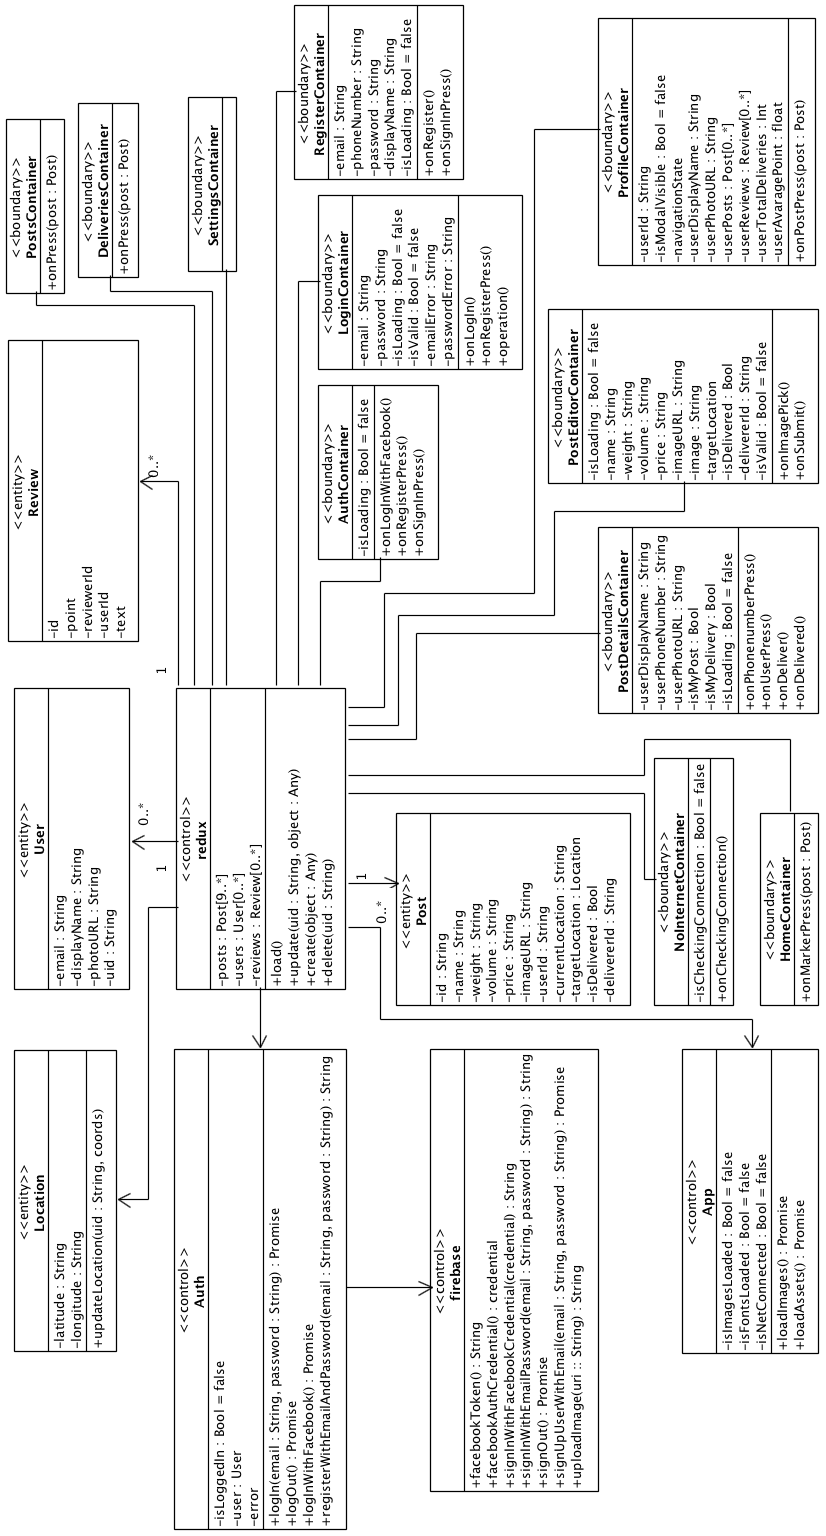
\includegraphics[height=.88\textheight]{Figures/shinjilgee/class_diagram.png}
	\caption{Шинжилгээнии класс диаграм}
\end{figure}

%-----------------------------------
%	SECTION 8
%-----------------------------------

\section{Шинжилгээний дарааллын диаграм}

\begin{figure}[H]
	\centering
	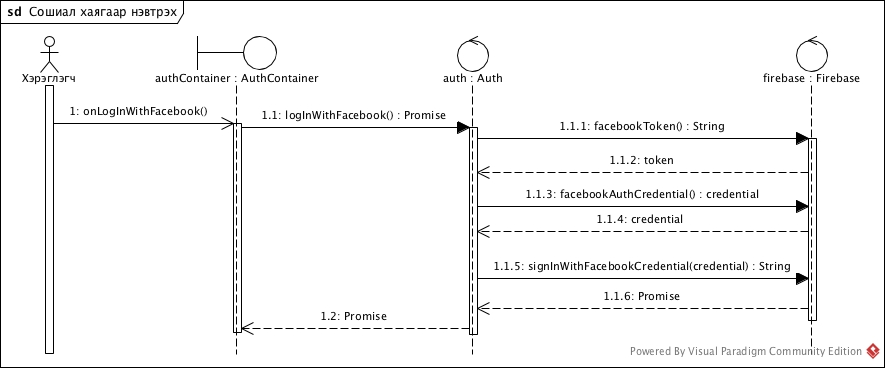
\includegraphics[width=\textwidth]{Figures/shinjilgee/seq/social_haygaar_nevtreh.jpg}
	\caption{Сошиал хаягаар нэвтрэх дарааллын диаграм}
\end{figure}

\begin{figure}[H]
	\centering
	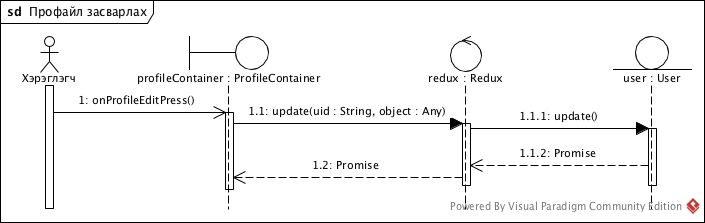
\includegraphics[width=\textwidth]{Figures/shinjilgee/seq/profile_zasvarlah.jpg}
  \caption{Профайл засварлах дарааллын диаграм}
\end{figure}

\begin{figure}[H]
	\centering
	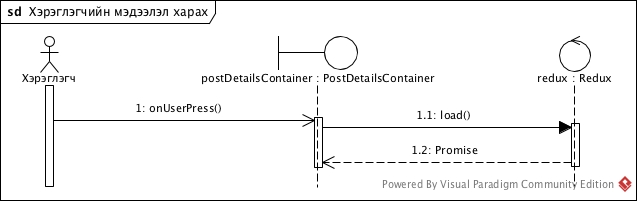
\includegraphics[width=\textwidth]{Figures/shinjilgee/seq/test.jpg}
  \caption{Хэрэглэгчийн мэдээлэл харах дарааллын диаграм}
\end{figure}

\begin{figure}[H]
	\centering
	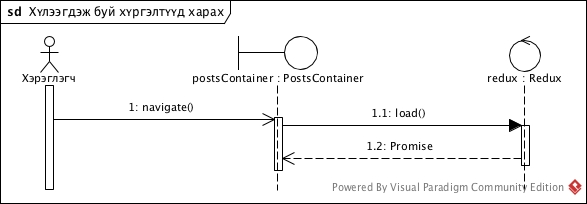
\includegraphics[width=\textwidth]{Figures/shinjilgee/seq/huleegdej_bui_hurgelt_harah.jpg}
  \caption{Хүлээгдэж буй хүргэлтүүд харах дарааллын диаграм}
\end{figure}

\begin{figure}[H]
	\centering
	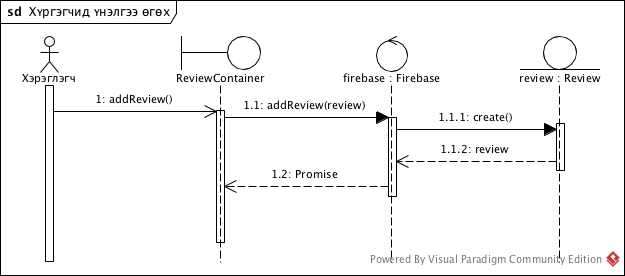
\includegraphics[width=\textwidth]{Figures/shinjilgee/seq/hurgegchid_unelgee_ogoh.jpg}
  \caption{Хүргэгчид үнэлгээ өгөх дарааллын диаграм}
\end{figure}

\begin{figure}[H]
	\centering
	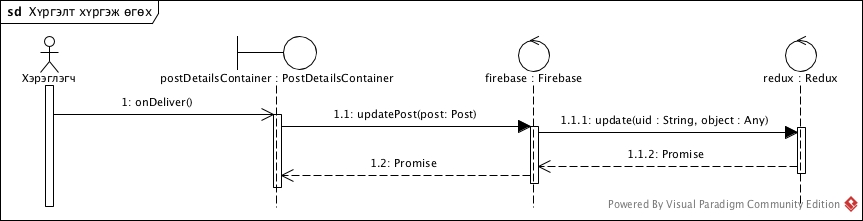
\includegraphics[width=\textwidth]{Figures/shinjilgee/seq/hurgelt_hurgej_ogoh.jpg}
  \caption{Хүргэлт хүргэж өгөх дарааллын диаграм}
\end{figure}

\begin{figure}[H]
	\centering
	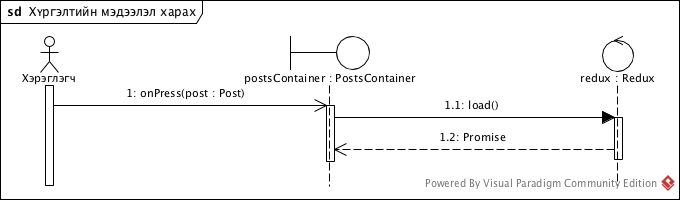
\includegraphics[width=\textwidth]{Figures/shinjilgee/seq/hurgeltiin_medeelel_harah.jpg}
  \caption{Хүргэлтийн мэдээлэл харах дарааллын диаграм}
\end{figure}

\begin{figure}[H]
	\centering
	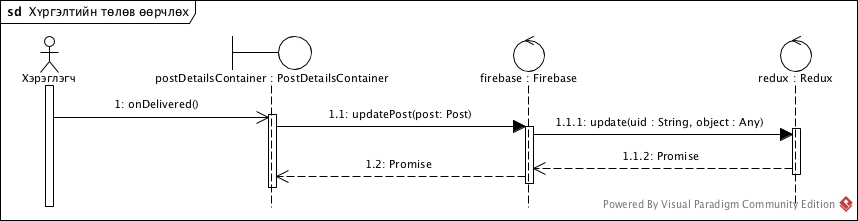
\includegraphics[width=\textwidth]{Figures/shinjilgee/seq/hurgeltiin_tolov_oorchloh.jpg}
  \caption{Хүргэлтийн төлөв өөрчлөх дарааллын диаграм}
\end{figure}

\begin{figure}[H]
	\centering
	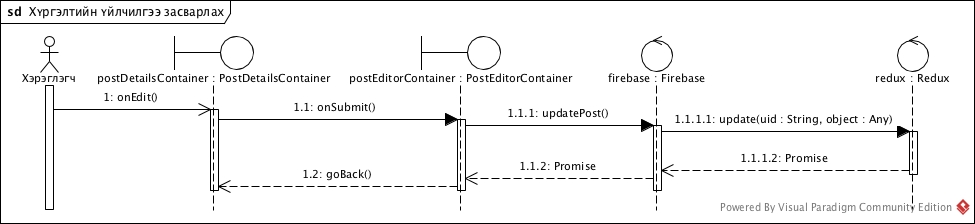
\includegraphics[width=\textwidth]{Figures/shinjilgee/seq/hurgeltiin_uilchilgee_zasvarlah.jpg}
  \caption{Хүргэлтийн үйлчилгээ засварлах дарааллын диаграм}
\end{figure}

\begin{figure}[H]
	\centering
	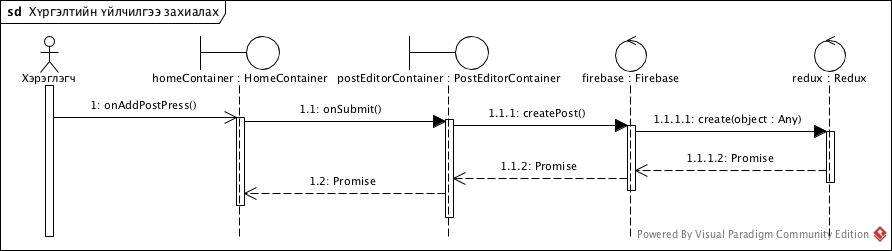
\includegraphics[width=\textwidth]{Figures/shinjilgee/seq/hurgeltiin_uilchilgee_zahialah.jpg}
  \caption{Хүргэлтийн үйлчилгээ захиалах дарааллын диаграм}
\end{figure}

\begin{figure}[H]
	\centering
	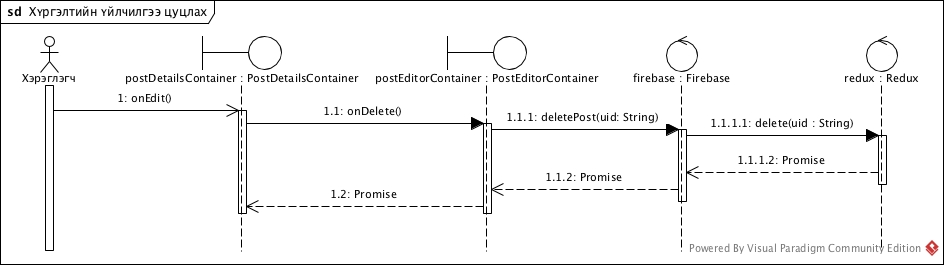
\includegraphics[width=\textwidth]{Figures/shinjilgee/seq/hurgeltiin_uilchilgee_tsutslah.jpg}
  \caption{Хүргэлтийн үйлчилгээ цуцлах дарааллын диаграм}
\end{figure}

%-----------------------------------
%	SECTION 9
%-----------------------------------

\section{Үйл ажиллагааны диаграм}

\begin{figure}[H]
  \centering
	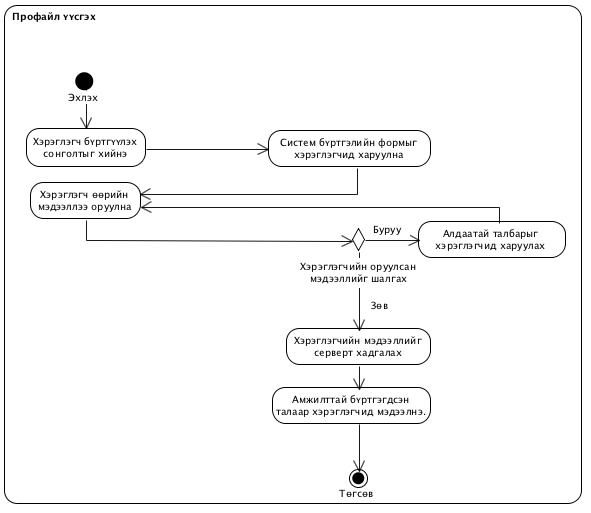
\includegraphics[width=\textwidth]{Figures/shinjilgee/activity/profile_uusgeh.png}
	\caption{Профайл үүсгэх үйл ажиллагааны диаграм}
\end{figure}

\begin{figure}[H]
  \centering
	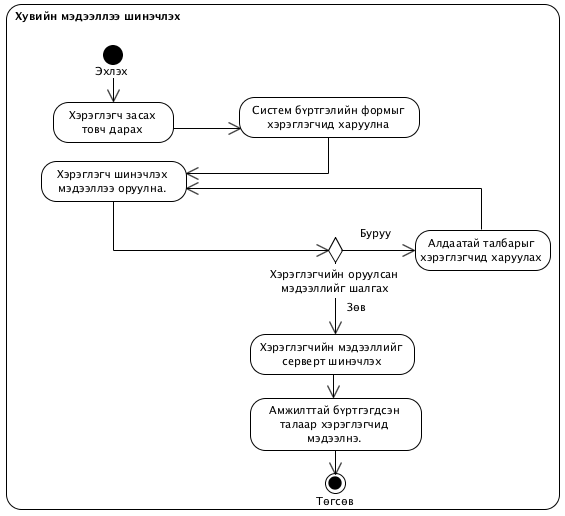
\includegraphics[width=\textwidth]{Figures/shinjilgee/activity/huviin_medeellee_shinchleh.png}
	\caption{Хувийн мэдээллээ шинэчлэх үйл ажиллагааны диаграм}
\end{figure}

\begin{figure}[H]
  \centering
	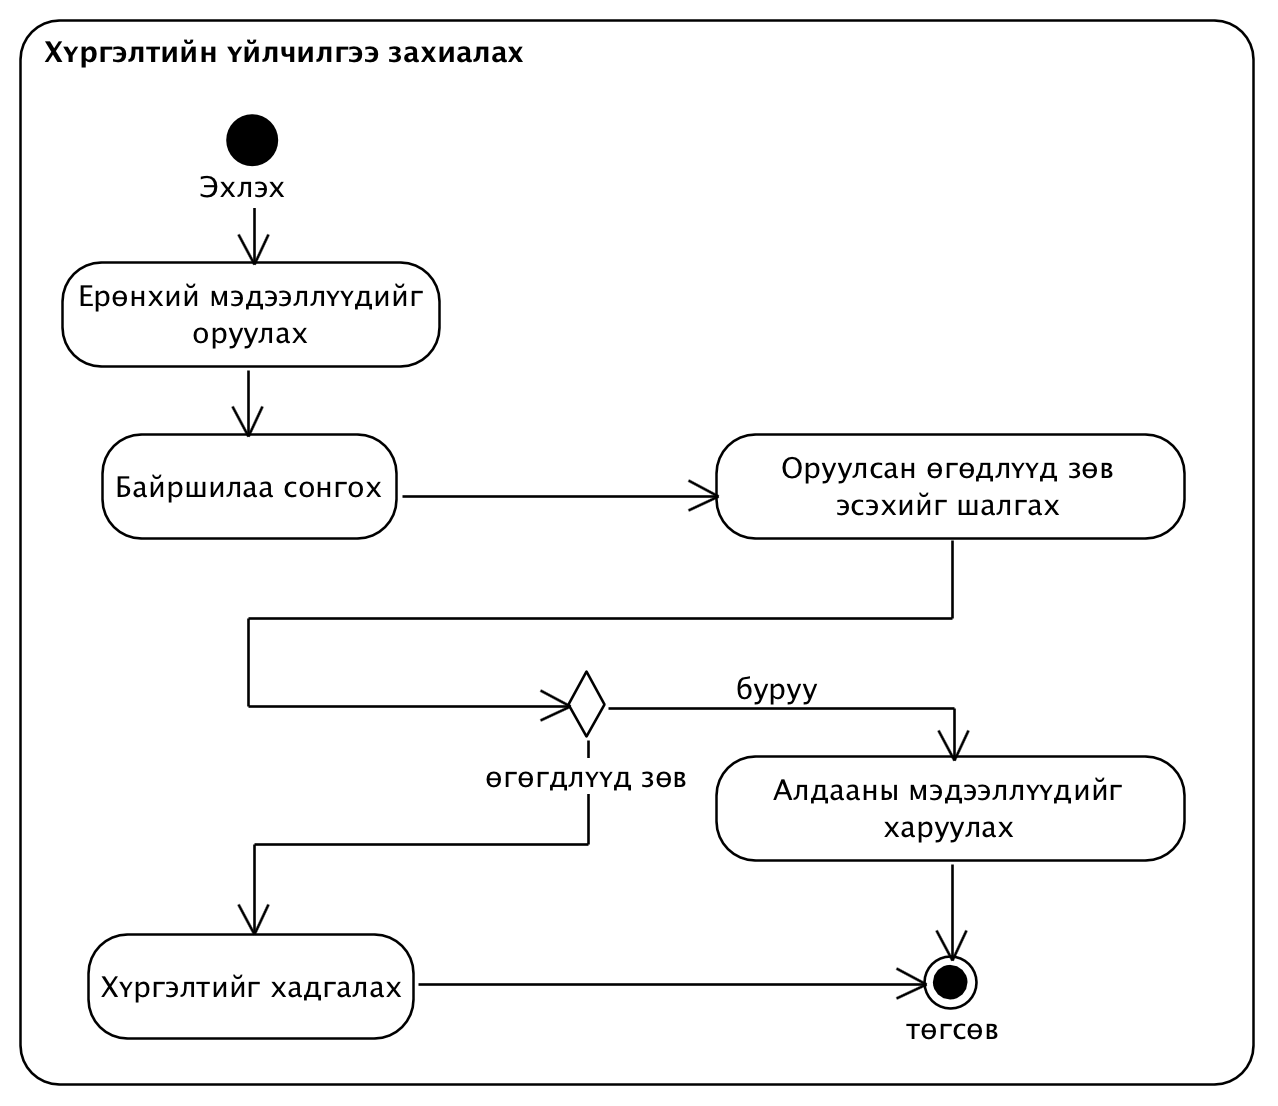
\includegraphics[width=\textwidth]{Figures/shinjilgee/activity/hurgeltiin_uilchilgee_zahialah.png}
	\caption{Хүргэлтийн үйлчилгээ захиалах үйл ажиллагааны диаграм}
\end{figure}

\begin{figure}[H]
  \centering
	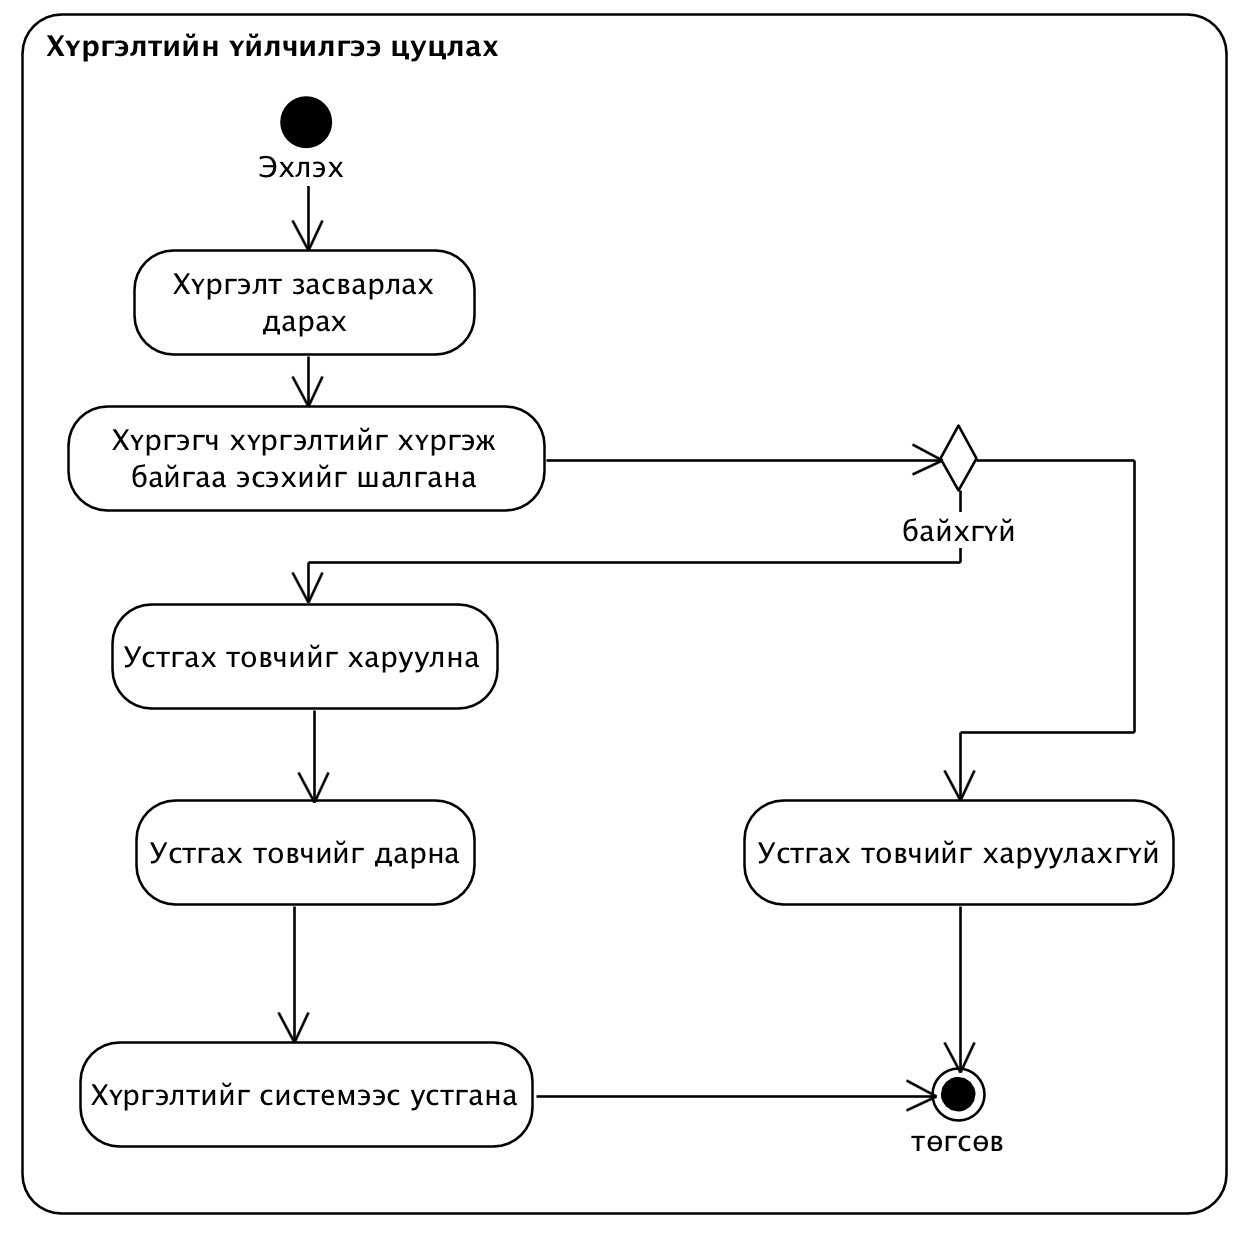
\includegraphics[width=\textwidth]{Figures/shinjilgee/activity/hurgeltiin_uilchilgee_tsutslah.png}
	\caption{Хүргэлтийн үйлчилгээ цуцлах үйл ажиллагааны диаграм}
\end{figure}

\begin{figure}[H]
  \centering
	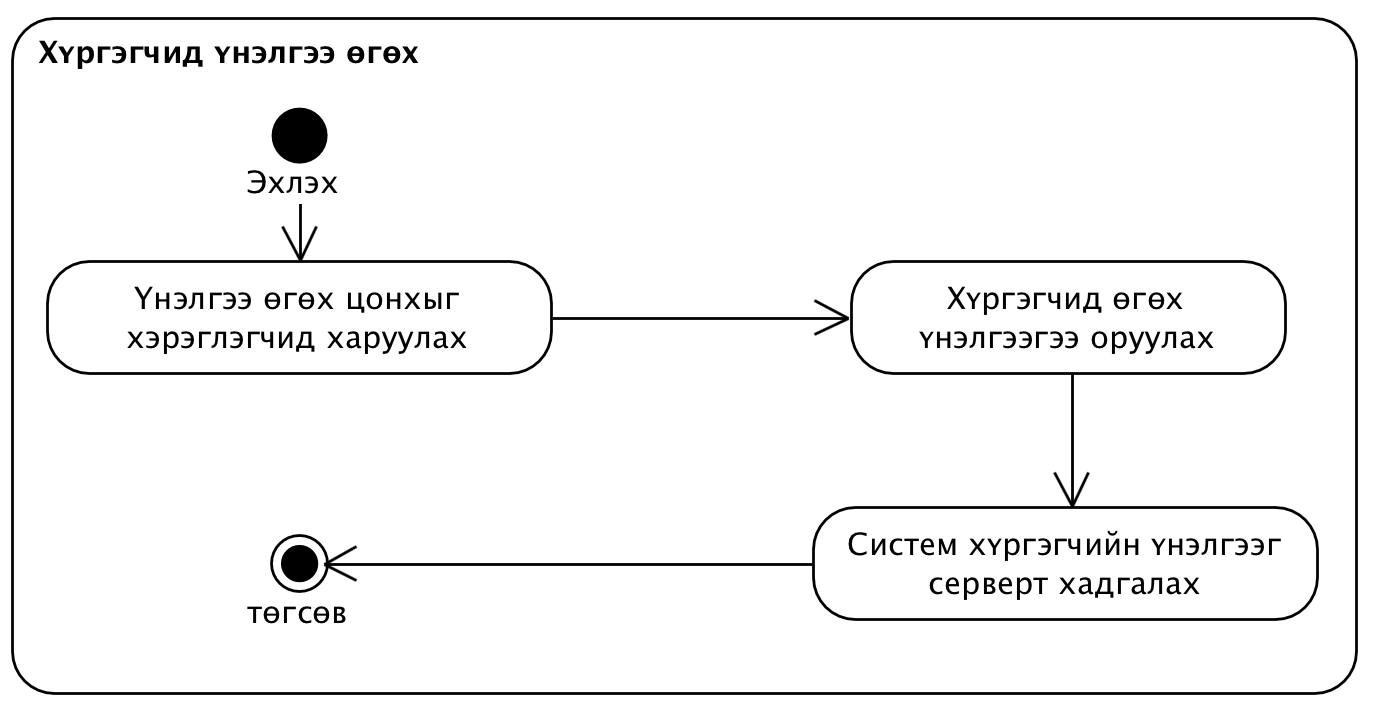
\includegraphics[width=\textwidth]{Figures/shinjilgee/activity/hurgegchid_unelgee_ogoh.png}
	\caption{Хүргэгчид үнэлгээ өгөх үйл ажиллагааны диаграм}
\end{figure}

\begin{figure}[H]
  \centering
	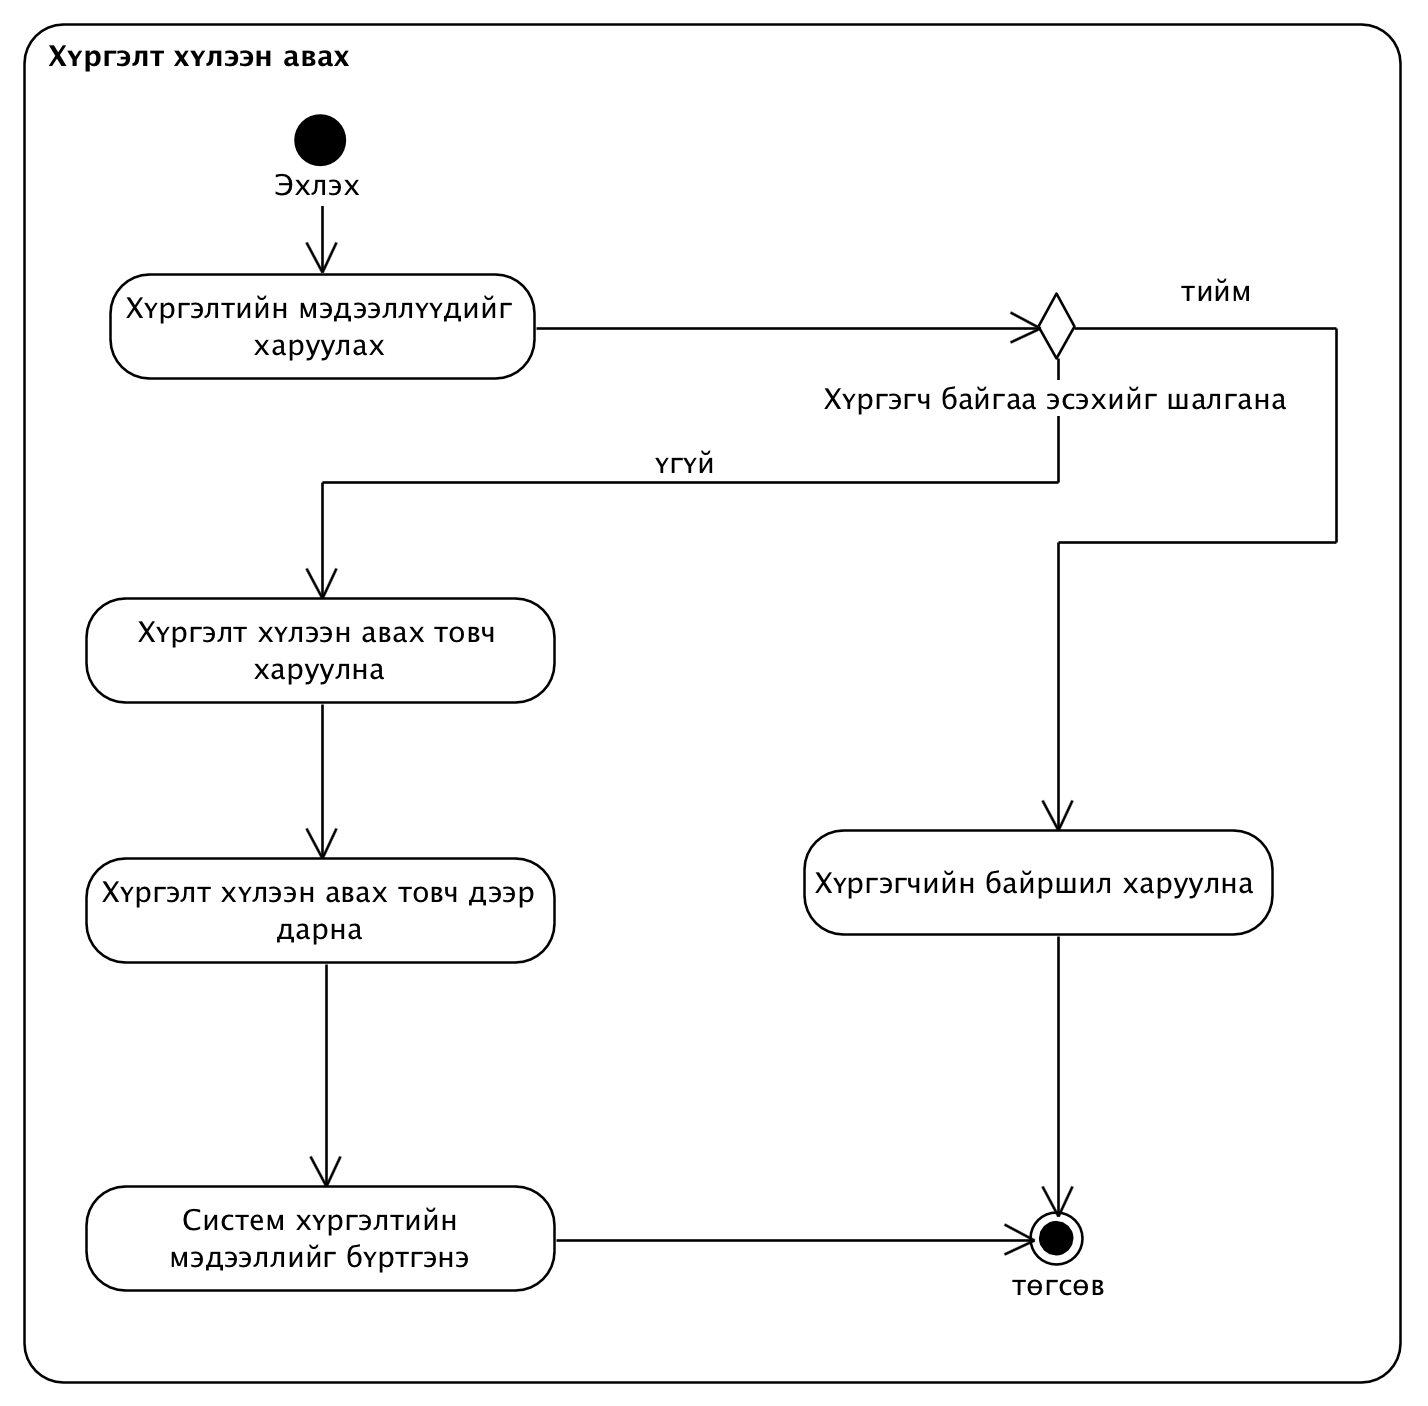
\includegraphics[width=\textwidth]{Figures/shinjilgee/activity/hurgelt_huleen_avah.png}
	\caption{Хүргэлт хүлээн авах үйл ажиллагааны диаграм}
\end{figure}

\begin{figure}[H]
  \centering
	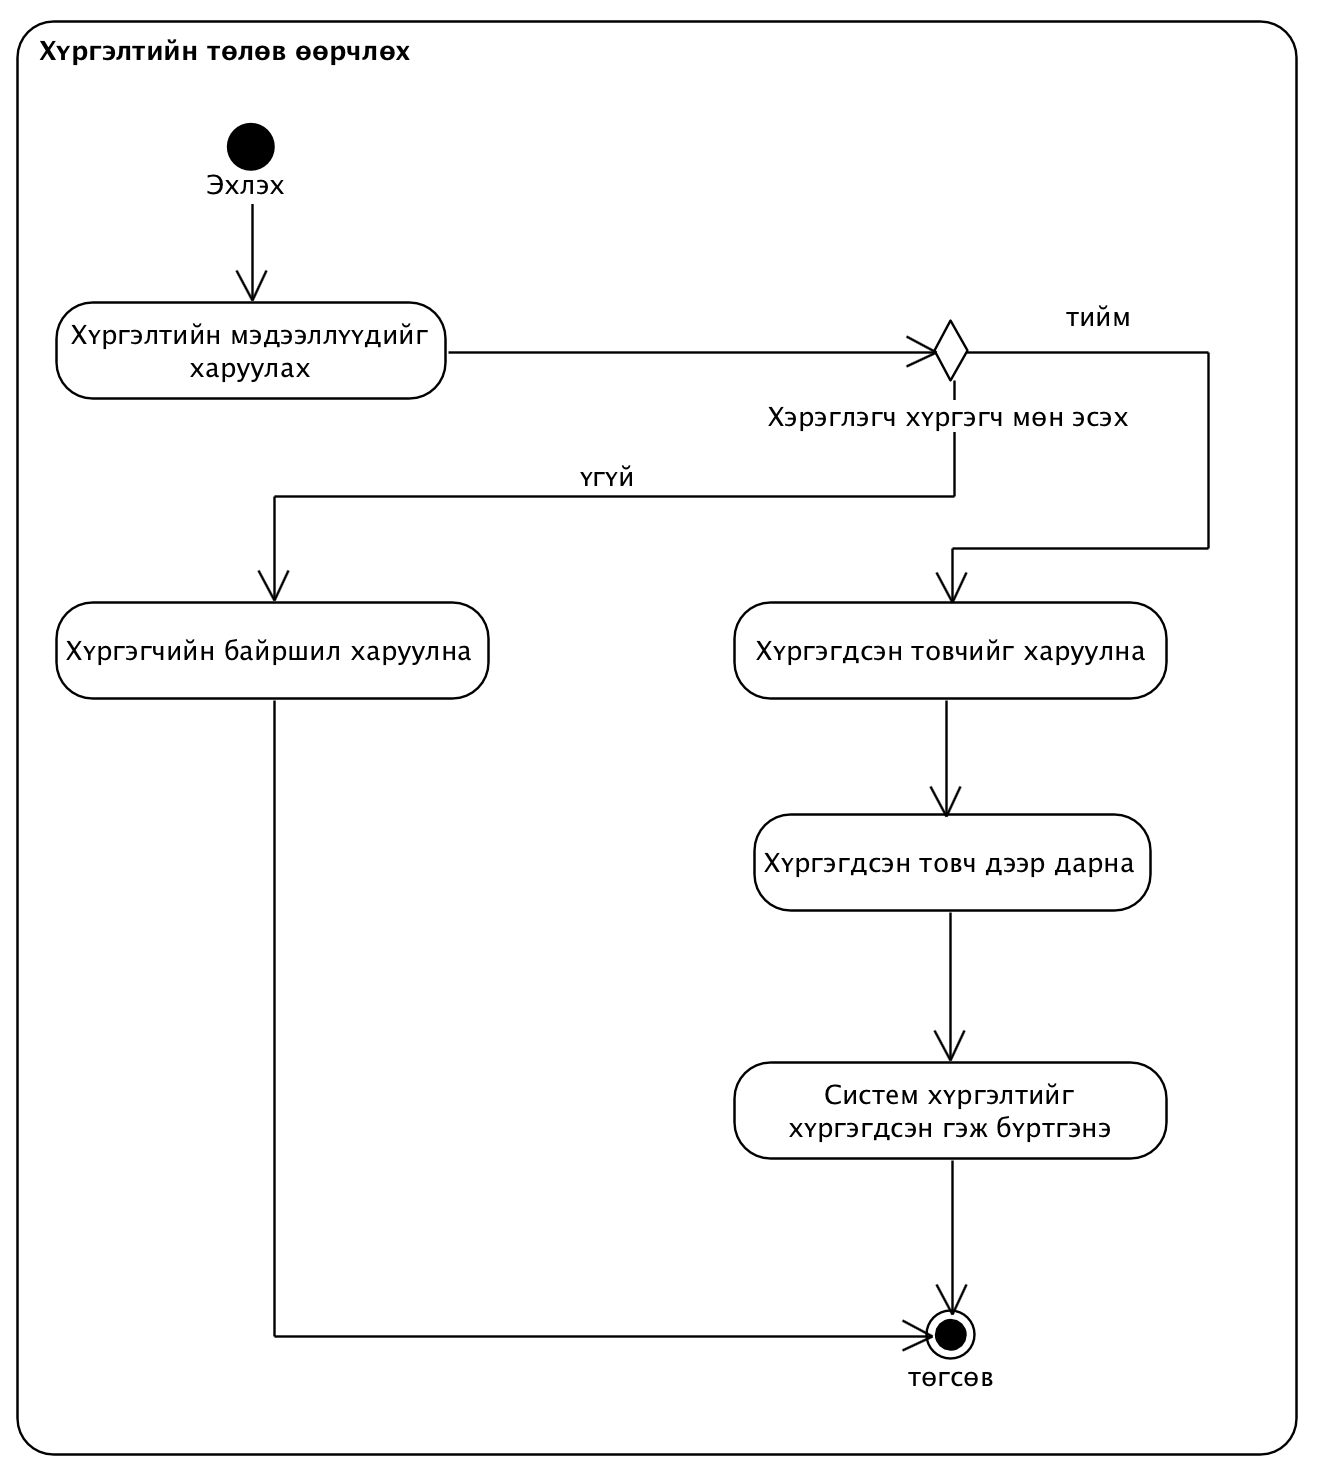
\includegraphics[width=\textwidth]{Figures/shinjilgee/activity/hurgeltiin_tolov_oorchloh.png}
	\caption{Хүргэлтийн төлөв өөрчлөх үйл ажиллагааны диаграм}
\end{figure}

%-----------------------------------
%	SECTION 10
%-----------------------------------

\section{Бүлгийн дүгнэлт}
Энэ бүлгийн хүрээнд уг системийн шаардлага болон шинжилгээний шатны бичиг баримтыг хийж гүйцэтгэсэн ба дараах зүйлсийг тодорхойлов:
\begin{itemize}[label={--}]
    \renewcommand\labelitemi{--}
    \item Системийн үйл ажиллагааг тодорхойлсон,
    \item Системийг ашиглах хэрэглэгчдийг тодорхойлсон,
    \item Функцийн шаардлагуудыг тодорхойлсон,
    \item Функцийн бус шаардлагуудыг тодорхойлсон,
    \item Юзкейс диаграмыг тодорхойлсон,
    \item Юзкейс тодорхойлолтуудыг тодорхойлсон,
    \item Шинжилгээний класс диаграмыг дүрсэлсэн,
    \item Шинжилгээний дарааллын диаграмыг дүрсэлсэн,
    \item Үйл ажиллагааны диаграмыг гаргасан болно.
\end{itemize} 
    % Бүлэг 3

\pagecolor{ChapterYellow}
\chapter{Зохиомж} % 3р бүлгийн нэр
\label{Chapter3} % Энэ бүлэг рүү ишлэл хийх бол \ref{Chapter2} командыг ашигла 

%-------------------------------------------------------------------------------
%	SECTION 1
%-------------------------------------------------------------------------------

\pagecolor{white}
\section{Өгөгдлийн ерөнхий схем}

\begin{figure}[H]
    \centering
    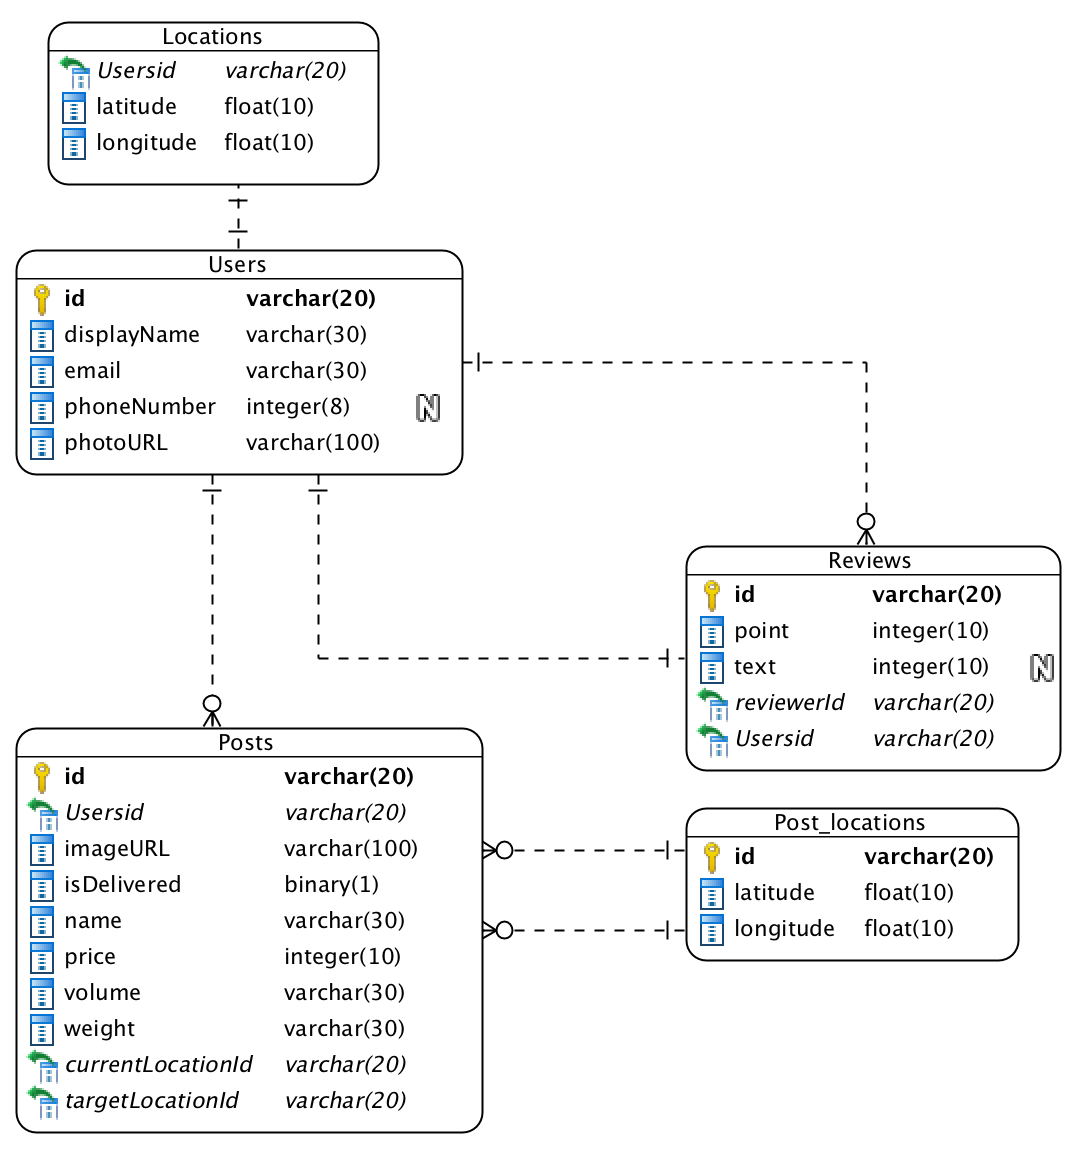
\includegraphics[width=\textwidth]{Figures/zohiomj/erd.png}
    \captionof{figure}{Өгөгдлийн ерөннхий схем}
\end{figure}

\section{Класс диаграм}

\begin{figure}[H]
    \centering
	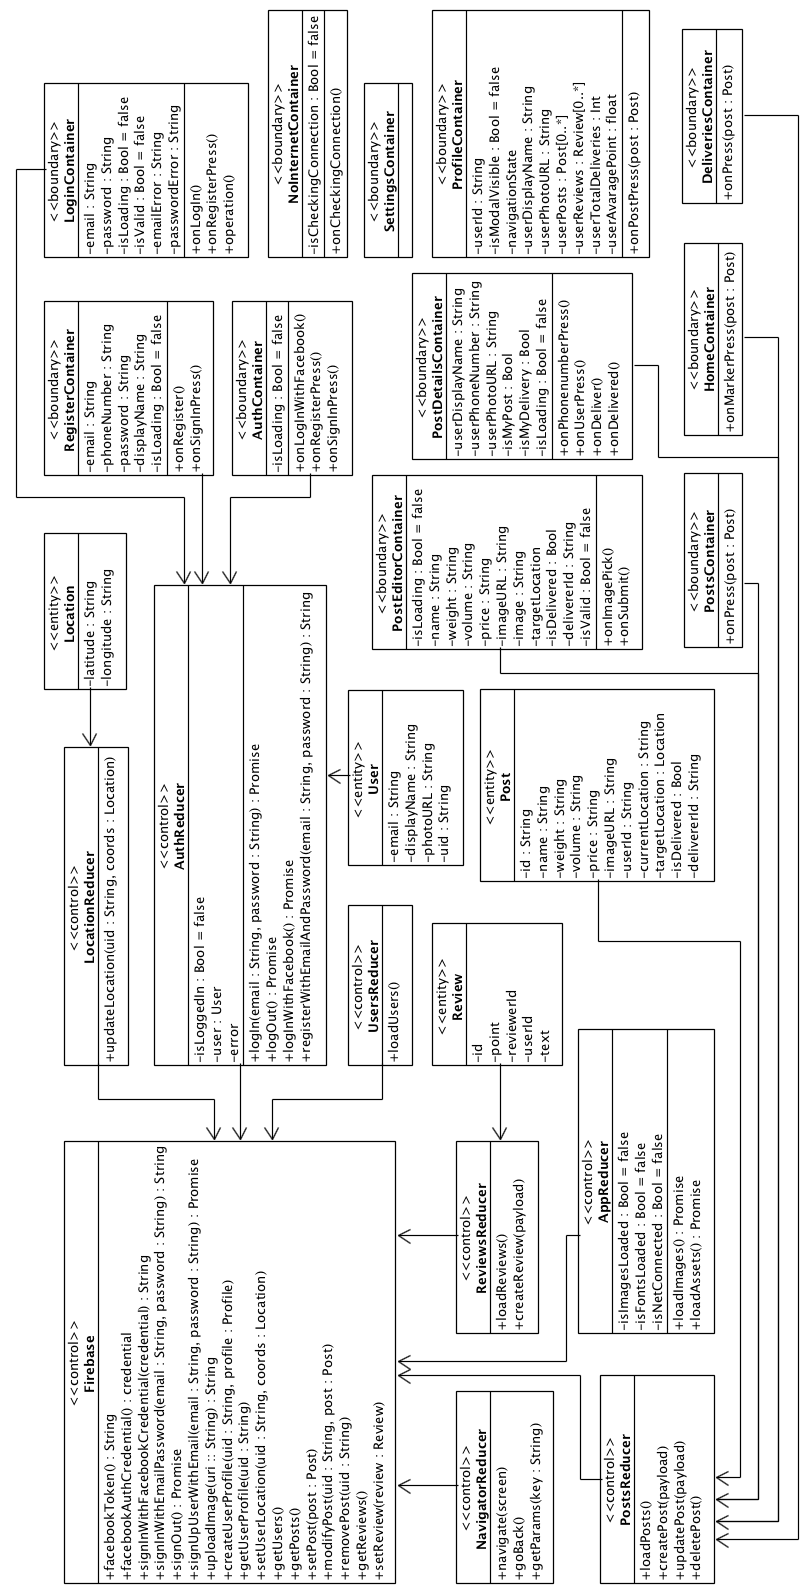
\includegraphics[height=.88\textheight]{Figures/zohiomj/upgraded_class.png}
    \captionof{figure}{Класс диаграм}
\end{figure}

% \begin{landscape} % Хуудсыг эргүүлэх

\section{Дарааллын диаграм}

\begin{figure}[H]
	\centering
	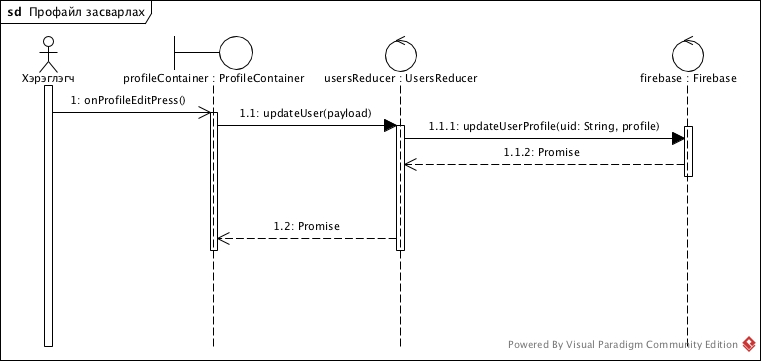
\includegraphics[width=\textwidth]{Figures/zohiomj/seq/profile_zasvarlah.jpg}
	\caption{Профайл засварлах дарааллын диаграм}
\end{figure}

\begin{figure}[H]
	\centering
	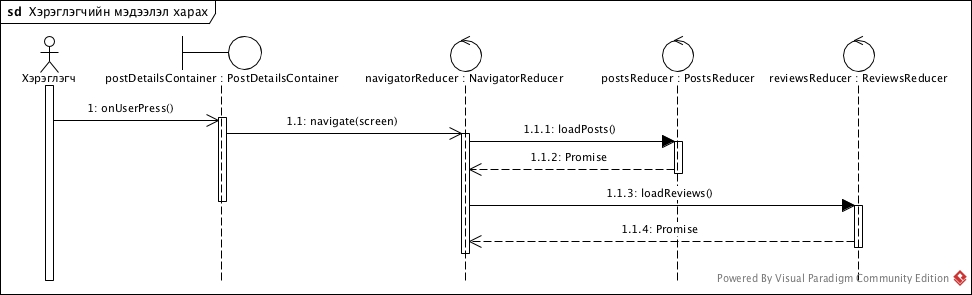
\includegraphics[width=\textwidth]{Figures/zohiomj/seq/hereglegchiin_medeelel_harah.jpg}
	\caption{Хэрэглэгчийн мэдээлэл харах дарааллын диаграм}
\end{figure}

\begin{figure}[H]
	\centering
	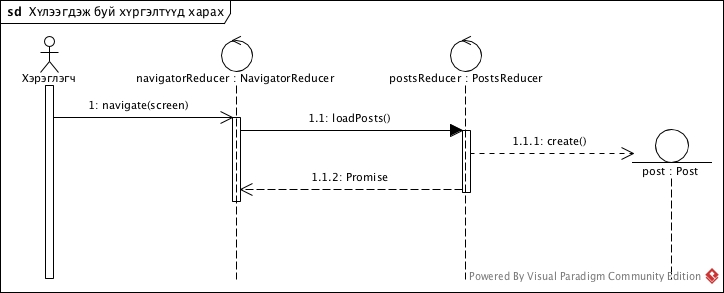
\includegraphics[width=\textwidth]{Figures/zohiomj/seq/huleegdej_bui_hurgelt_harah.jpg}
	\caption{Хүлээгдэж буй хүргэлтүүд харах дарааллын диаграм}
\end{figure}

\begin{figure}[H]
	\centering
	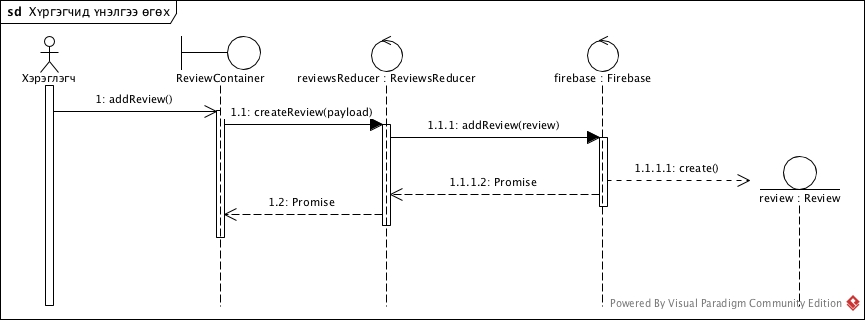
\includegraphics[width=\textwidth]{Figures/zohiomj/seq/hurgegchid_unelgee_ogoh.jpg}
	\caption{Хүргэгчид үнэлгээ өгөх дарааллын диаграм}
\end{figure}

\begin{figure}[H]
	\centering
	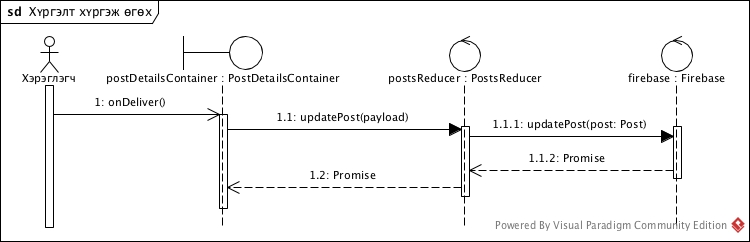
\includegraphics[width=\textwidth]{Figures/zohiomj/seq/hurgelt_hurgej_ogoh.jpg}
	\caption{Хүргэлт хүргэж өгөх дарааллын диаграм}
\end{figure}

\begin{figure}[H]
	\centering
	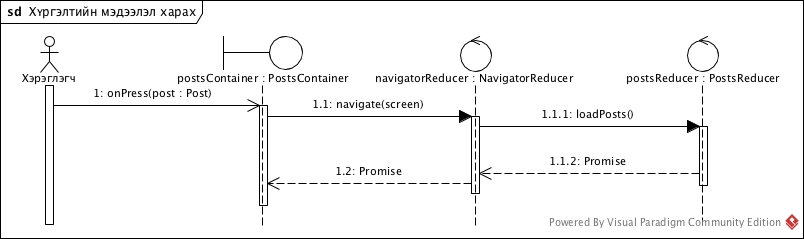
\includegraphics[width=\textwidth]{Figures/zohiomj/seq/hurgeltiin_medeelel_harah.jpg}
	\caption{Хүргэлтийн мэдээлэл харах дарааллын диаграм}
\end{figure}

\begin{figure}[H]
	\centering
	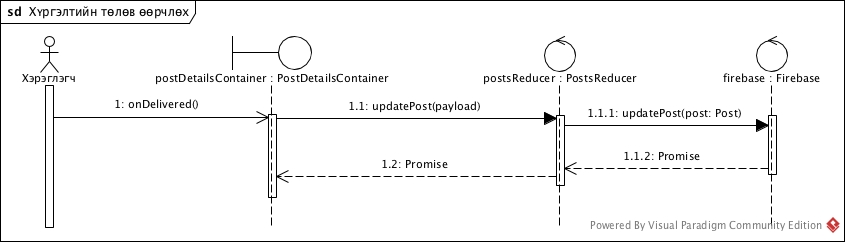
\includegraphics[width=\textwidth]{Figures/zohiomj/seq/hurgeltiin_tolov_oorchloh.jpg}
	\caption{Хүргэлтийн төлөв өөрчлөх дарааллын диаграм}
\end{figure}

\begin{figure}[H]
	\centering
	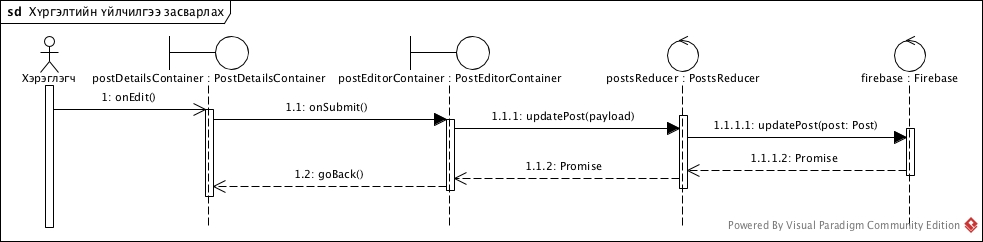
\includegraphics[width=\textwidth]{Figures/zohiomj/seq/hurgeltiin_uilchilgee_zasvarlah.jpg}
	\caption{Хүргэлтийн үйлчилгээ засварлах дарааллын диаграм}
\end{figure}

\begin{figure}[H]
	\centering
	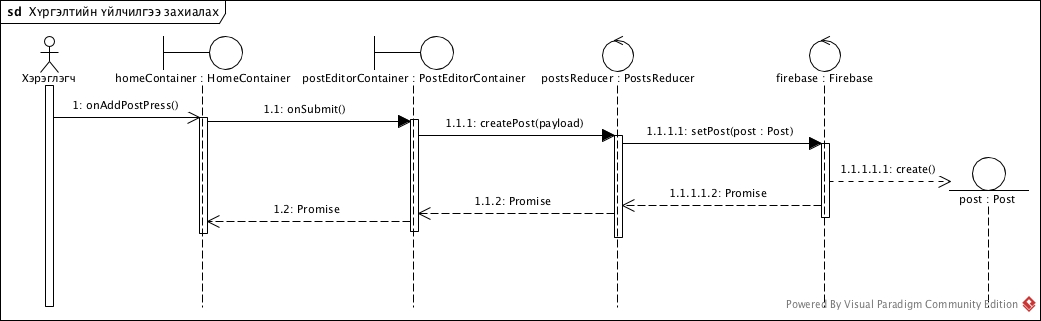
\includegraphics[width=\textwidth]{Figures/zohiomj/seq/hurgeltiin_uilchilgee_zahialah.jpg}
	\caption{Хүргэлтийн үйлчилгээ захиалах дарааллын диаграм}
\end{figure}

\begin{figure}[H]
	\centering
	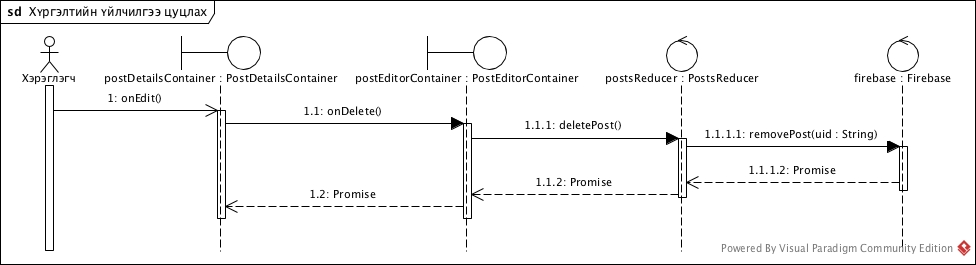
\includegraphics[width=\textwidth]{Figures/zohiomj/seq/hurgeltiin_uilchilgee_tsutslah.jpg}
	\caption{Хүргэлтийн үйлчилгээ цуцлах дарааллын диаграм}
\end{figure}

% \end{landscape}


% \begin{landscape} % Хуудсыг эргүүлэх
\section{Хэрэглэгчийн интерфейс}

\begin{figure}[H]
	\centering
    \subcaptionbox{Анхны дэлгэц}{
        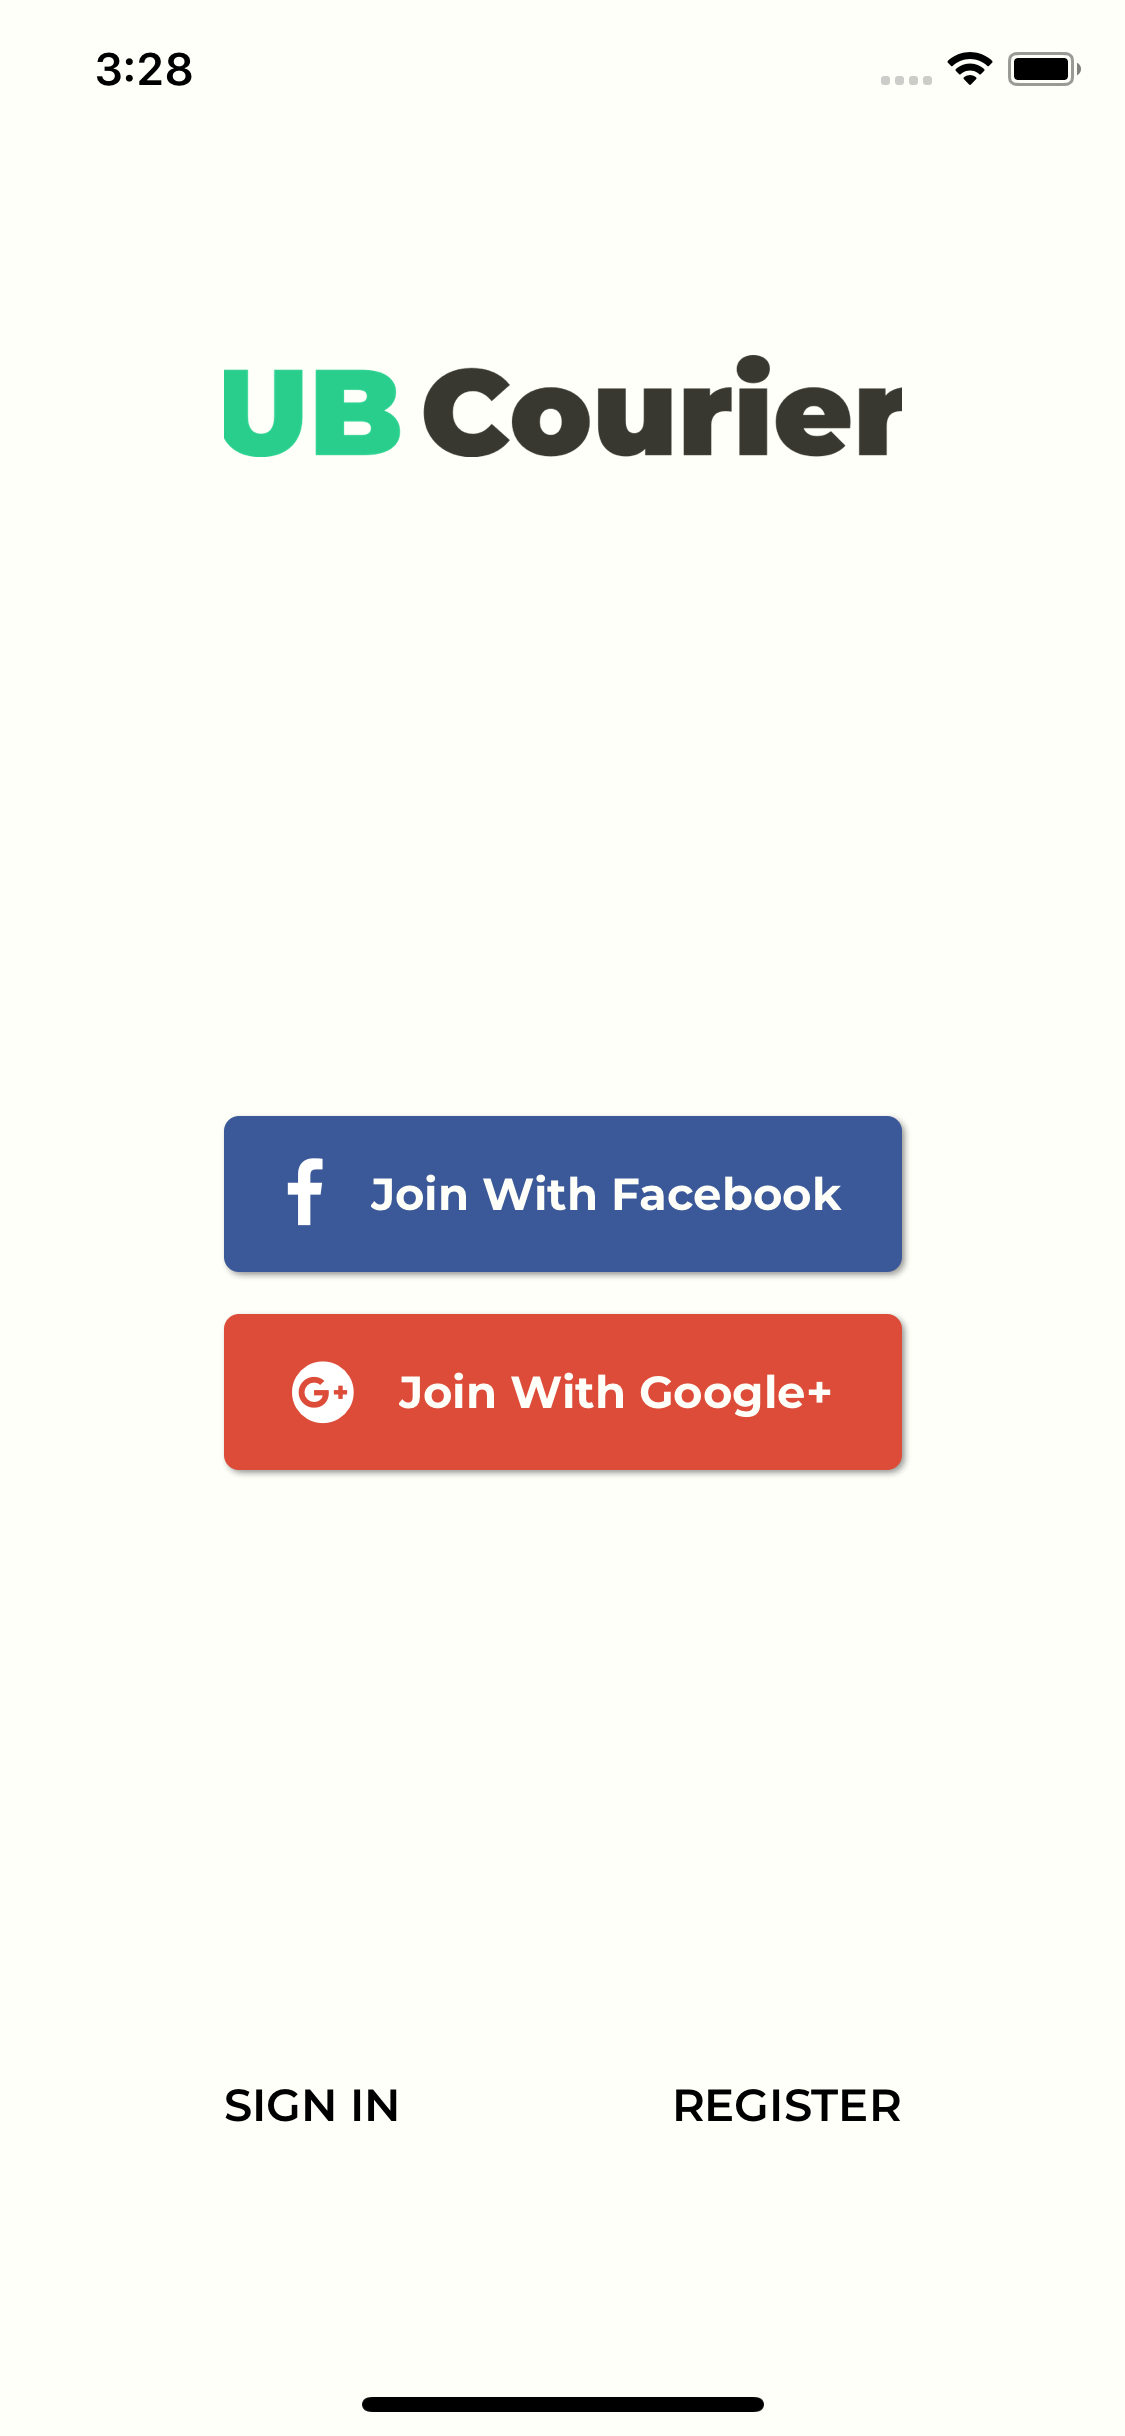
\includegraphics[height=.41\textheight, frame]{Figures/interfaces/interface1.png}
    }
    \hfill
    \subcaptionbox{Нэвтрэх дэлгэц}{
        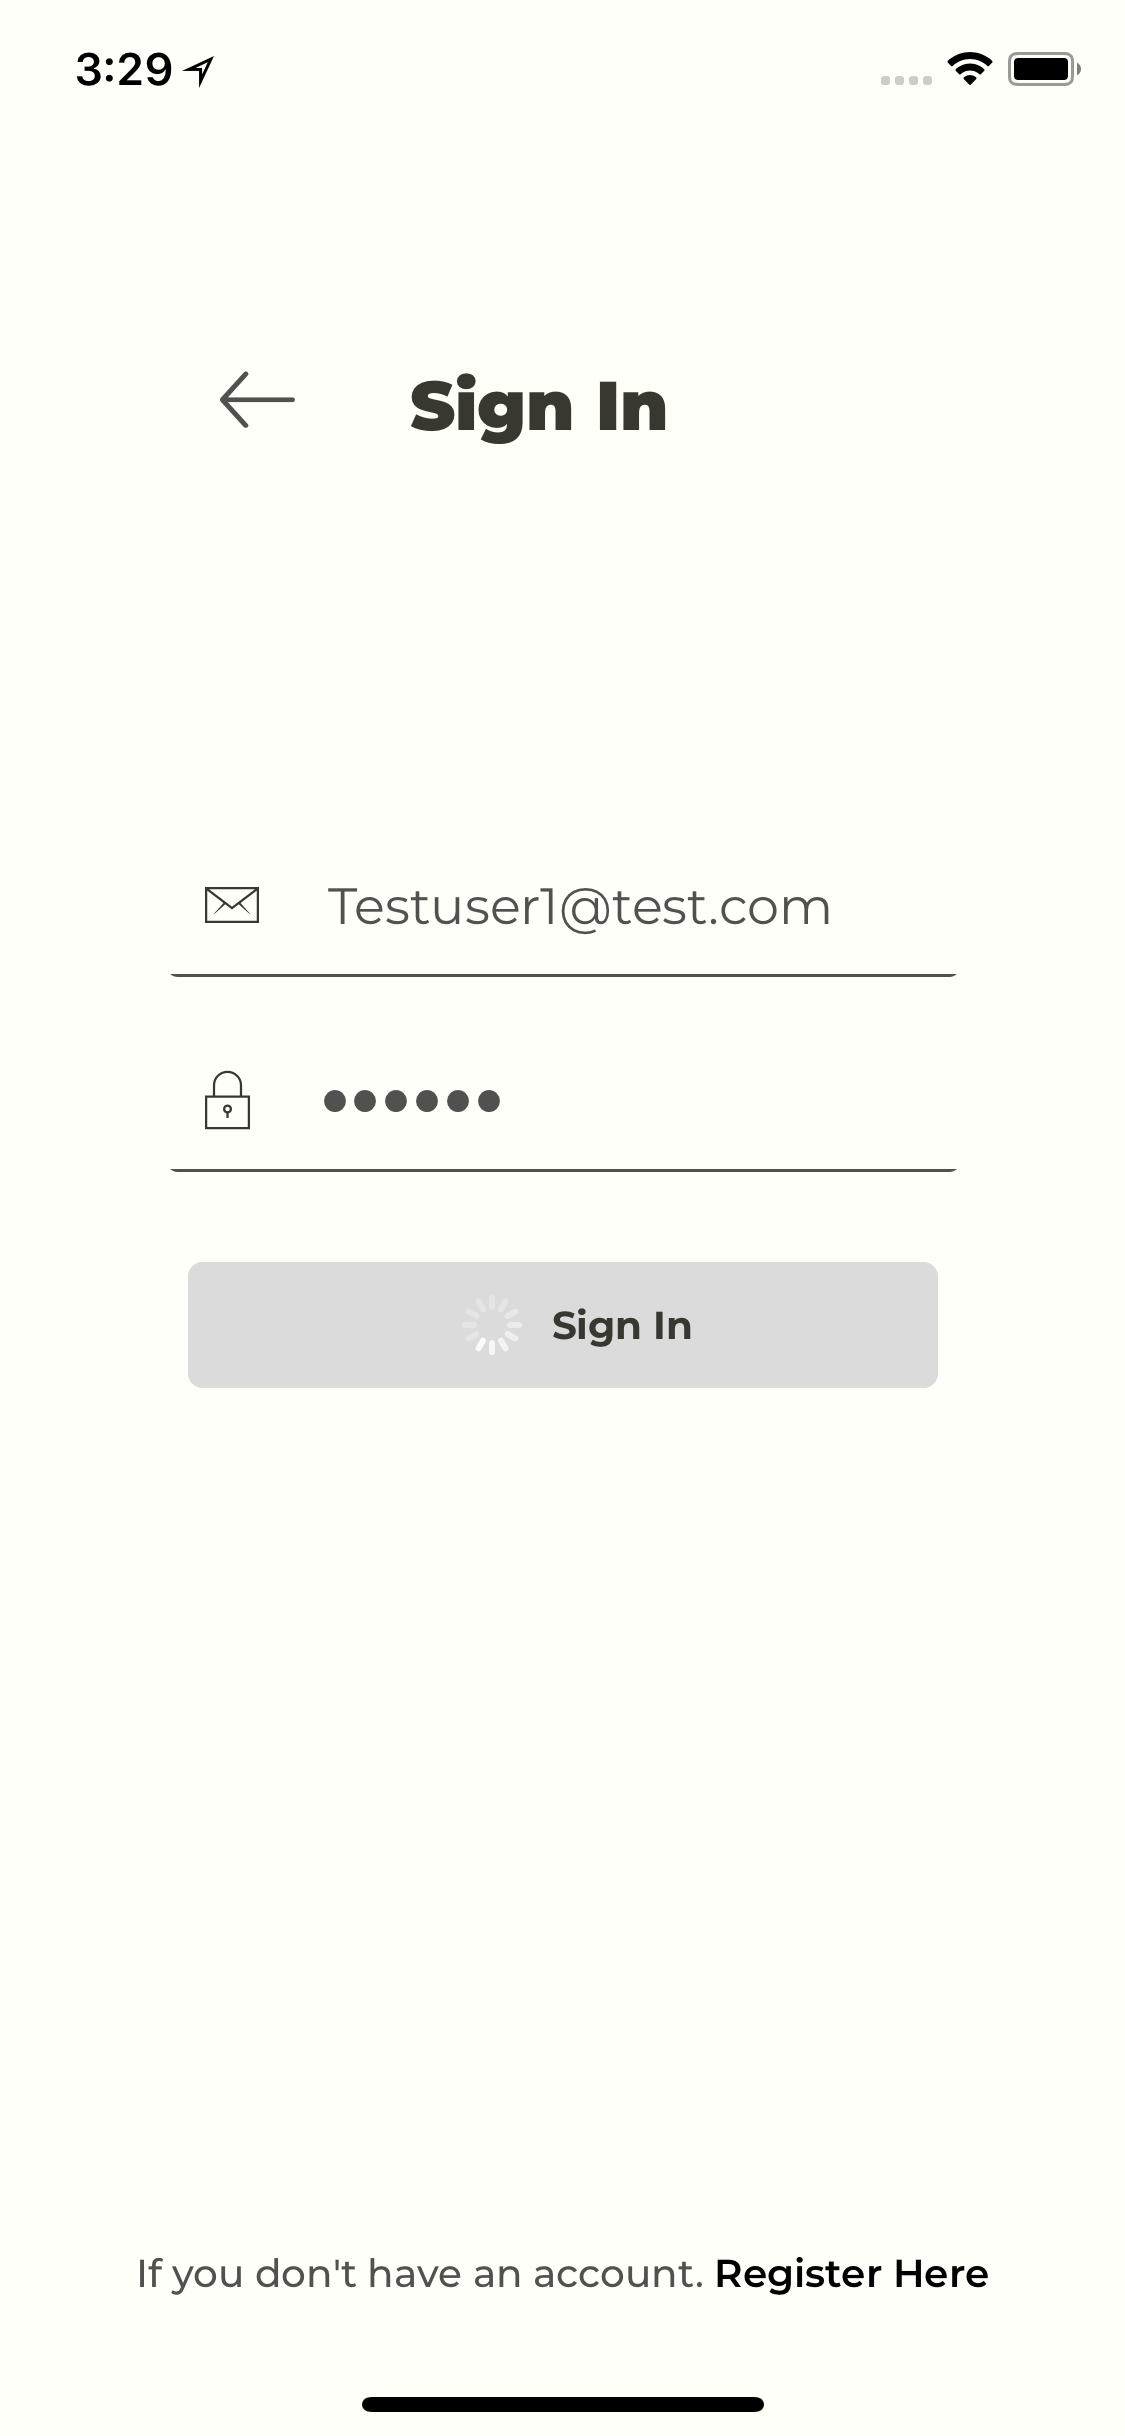
\includegraphics[height=.41\textheight, frame]{Figures/interfaces/interface2.png}
    }
    \subcaptionbox{Бүртгүүлэх дэлгэц}{
        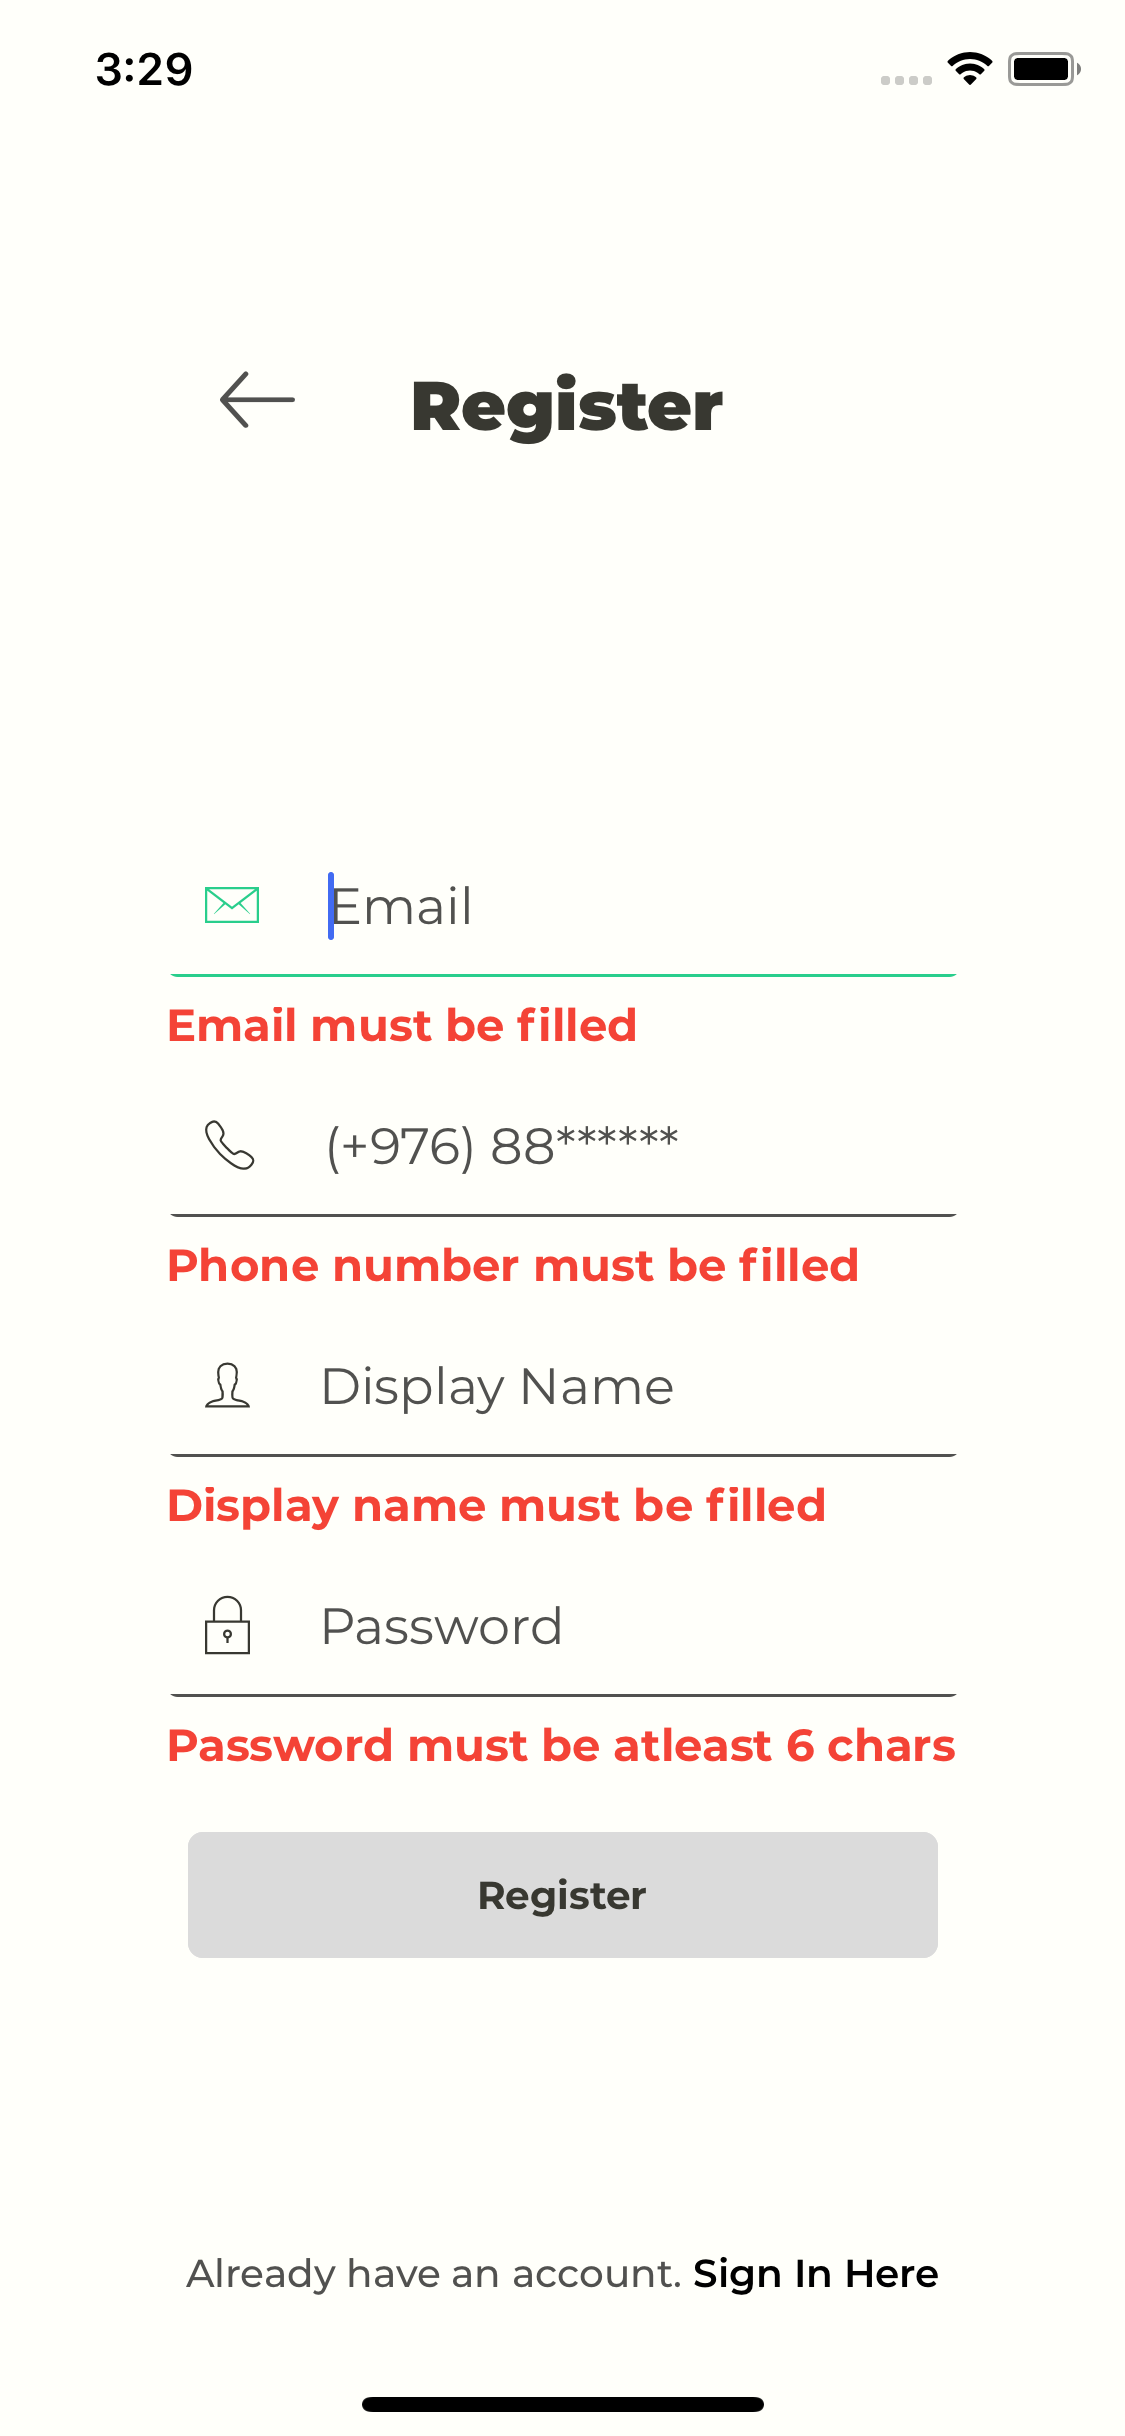
\includegraphics[height=.41\textheight, frame]{Figures/interfaces/interface3.png}
    }
    \hfill
    \subcaptionbox{Facebook нэвтрэх}{
        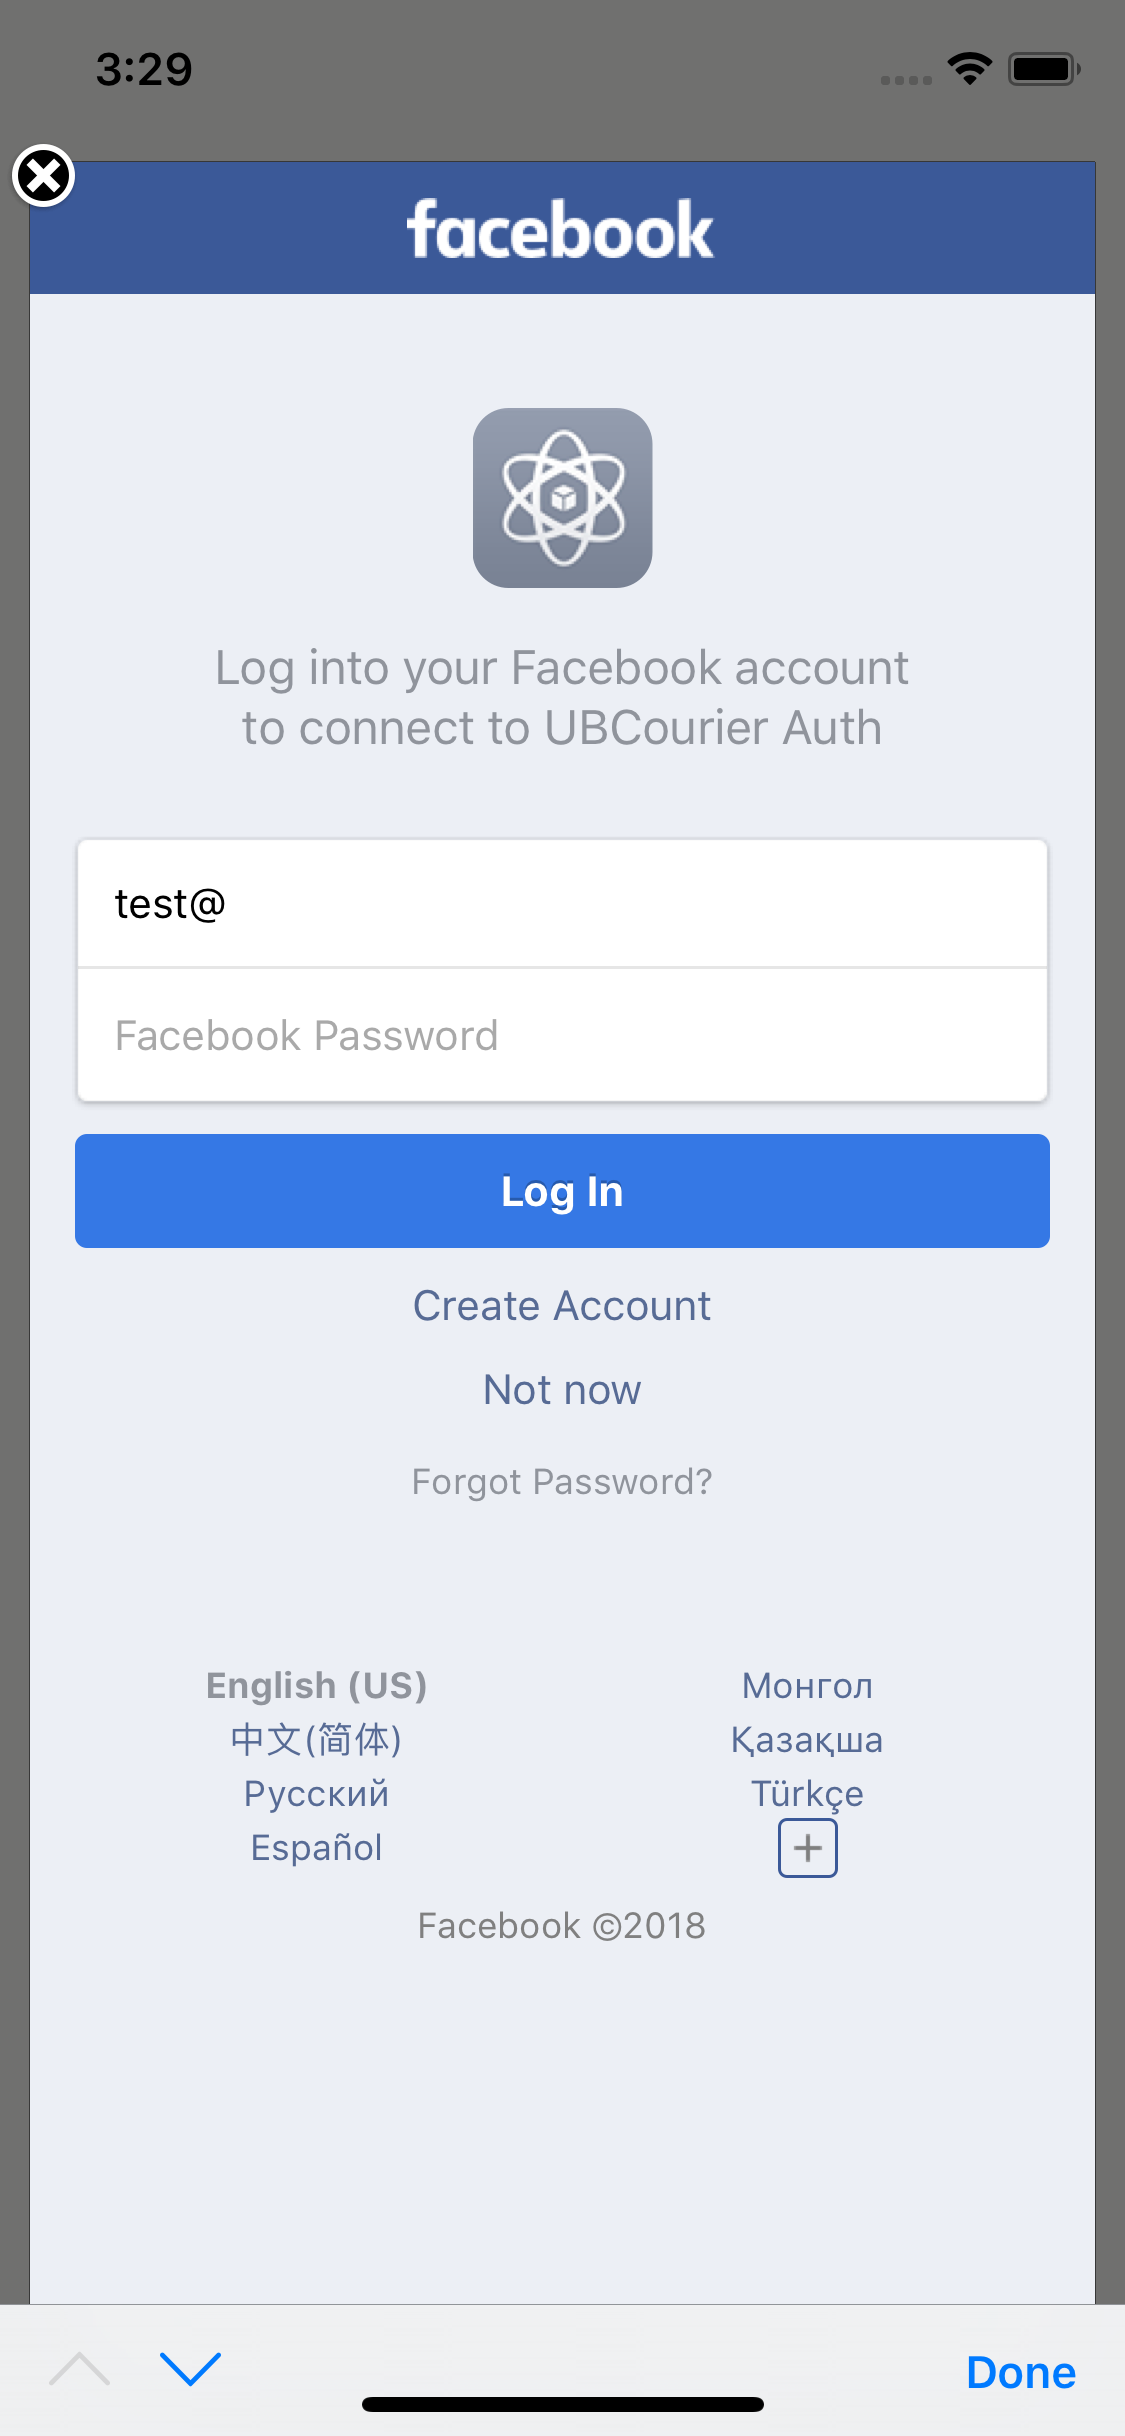
\includegraphics[height=.41\textheight, frame]{Figures/interfaces/interface4.png}
    }
    \hfill
	\caption{Нэвтрэх болон бүртгүүлэх дэлгэцийн интерфейс}
\end{figure}

\begin{figure}[H]
	\centering
    \subcaptionbox{Нэвтэрсний дараах дэлгэц}{
        \includegraphics[width=.45\textwidth, frame]{Figures/interfaces/interface5.png}
    }
    \hfill
    \subcaptionbox{Цэсийн дэлгэсэн байдал}{
        \includegraphics[width=.45\textwidth, frame]{Figures/interfaces/interface6.png}
    }
	\caption{Үндсэн дэлгэц болон цэсний интерфейс}
\end{figure}

\begin{figure}[H]
	\centering
    \subcaptionbox{Миний хүргэлтийн захиалгууд}{
        \includegraphics[width=.3\textwidth, frame]{Figures/interfaces/interface7.png}
    }
    \hfill
    \subcaptionbox{Миний хүргэлтүүд}{
        \includegraphics[width=.3\textwidth, frame]{Figures/interfaces/interface8.png}
    }
    \hfill
    \subcaptionbox{Шинэ захиалга}{
        \includegraphics[width=.3\textwidth, frame]{Figures/interfaces/interface9.png}
    }
	\caption{Хүргэлтүүдийн дэлгэцийн интерфэйс}
\end{figure}

\begin{figure}[H]
	\centering
    \subcaptionbox{Миний хүргэлт}{
        \includegraphics[width=.3\textwidth, frame]{Figures/interfaces/interface10.png}
    }
    \hfill
    \subcaptionbox{Миний хүргэлтийн захиалга}{
        \includegraphics[width=.3\textwidth, frame]{Figures/interfaces/interface11.png}
    }
    \hfill
    \subcaptionbox{Хүргэгчгүй хүргэлт}{
        \includegraphics[width=.3\textwidth, frame]{Figures/interfaces/interface12.png}
    }
	\caption{Хүргэлтийн мэдээллүүд дэлгэцийн интерфэйс}
\end{figure}

\begin{figure}[H]
	\centering
    \subcaptionbox{Хэрэглэгчийн хүргэлтүүд}{
        \includegraphics[width=.45\textwidth, frame]{Figures/interfaces/interface12.png}
    }
    \hfill
    \subcaptionbox{Хэрэглэгчийн үнэлгээнүүд}{
        \includegraphics[width=.45\textwidth, frame]{Figures/interfaces/interface13.png}
    }
	\caption{Хэрэглэгчийн профайл дэлгэцийн интерфэйс}
\end{figure}

% \end{landscape} % Хуудсыг эргүүлэх

\section{Бүлгийн дүгнэлт}
Энэ бүлгийн хүрээнд уг төслийн ажлын зохиомжийн шатны бичиг баримтыг хийж гүйцэтгэсэн ба дараах зүйлсийг тодорхойлов:
\begin{itemize}[label={--}]
    \renewcommand\labelitemi{--}
    \item Өгөгдлийн ерөнхий схемийг гаргасан,
    \item Класс диаграмыг дүрсэлсэн,
    \item Дарааллын диаграмыг дүрсэлсэн,
    \item Хэрэглэгчийн интерфейсийг дүрсэлсэн болно.
\end{itemize}

    %\include{Chapters/Chapter4} 
    %\include{Chapters/Chapter5}
    
    % Дүгнэлт бүлэг
    %-------------------------------------------------------------------------------
%	CONCLUSION
%-------------------------------------------------------------------------------

\begin{conclusion}
\addchaptertocentry{\conclusionname}

Энэхүү бакалаврын төгсөлтийн ажлын хүрээнд хүргэлтийн үйлчилгээ авах хүмүүст зориулан хүргэлтийн үйлчилгээний систем хөгжүүлэхийг зорьж системийн бичиг баримтыг бэлтгэн дараах зүйлсийг тодорхойлов:
\begin{itemize}[label={--},nosep]
	\item Системийн үйл ажиллагаа болон хамрах хүрээг өөрийн системийн онцлогт тааруулан бүтэцлэн тодорхойлсон,
    \item Системийн үйл ажиллагааг тодорхойлсон,
    \item Системийг ашиглах хэрэглэгчдийг тодорхойлсон,
    \item Системийн шаардлагуудыг тодорхойлсон,
	\item Дээрх шинжилгээнүүд дээр тулгуурлан системийн юзкейс диаграмыг дүрсэлсэн,
	\item Дүрсэлсэн юзкейс диаграмын юзкейс тус бүрийн тодорхойлолтыг гаргасан,
    \item Шинжилгээний класс диаграмыг дүрсэлсэн,
    \item Шинжилгээний дарааллын диаграмыг дүрсэлсэн,
    \item Үйл ажиллагааны диаграмыг дүрсэлсэн,
    \item Системийн өгөгдлийн ерөнхий схемийг гаргасан,
    \item Системийн класс диаграмыг дүрсэлсэн,
    \item Системийн дарааллын диаграмыг дүрсэлсэн,
    \item Системийг хэрэглэгчийн интерфейсийг дүрслэн бэлтгэсэн,
    \item бакалаврын төгсөлтийн ажлын бичиг баримтыг \LaTeX  ашиглаж бэлтгэсэн болно.
\end{itemize}

\end{conclusion} % Дүгнэлт
    
    
    %-------------------------------------------------------------------------------
    %	THESIS CONTENT - APPENDICES
    %-------------------------------------------------------------------------------
    
    \appendix % Дараах "chapters" нь Хавсралт болохыг LaTex -д хэлэх
    
    % Тезисийн бүлгүүдийг Appendices хавтаснаас бие даасан файл байдлаар оруулах
    
    %% Хавсралт A

\chapter{Хавсралтын нэр} % Main appendix title

\label{AppendixA} % For referencing this appendix elsewhere, use \ref{AppendixA}

Хавсралтаа энд бичнэ.
    %\include{Appendices/AppendixB}
    %\include{Appendices/AppendixC}
    
    %-------------------------------------------------------------------------------
    %	BIBLIOGRAPHY
    %-------------------------------------------------------------------------------
    \defformat % Бүлгийн нэрийг оргиналь байдлаар хэвлэх
    
    \addchaptertocentry{Ашигласан материалын жагсаалт} % Ном зүйг гарчигт нэмэх
    
    \printbibliography[heading=bibliography,title={Ашигласан материалын жагсаалт}]
    
    %-------------------------------------------------------------------------------

\end{document}  
 